
%\documentclass{tufte-book}
\documentclass[a4paper,twoside,fleqn]{tufte-book}
\setcounter{secnumdepth}{2}

\usepackage[
    type={CC},
    modifier={by-sa},
    version={3.0},
]{doclicense}

\hypersetup{colorlinks}% uncomment this line if you prefer colored hyperlinks (e.g., for onscreen viewing)

%%
% Book metadata
\title{Practical Grid\\Modelling}
\author[]{Santiago Pe\~nate Vera}
\publisher{}

%%
% If they're installed, use Bergamo and Chantilly from www.fontsite.com.
% They're clones of Bembo and Gill Sans, respectively.
%\IfFileExists{bergamo.sty}{\usepackage[osf]{bergamo}}{}% Bembo
%\IfFileExists{chantill.sty}{\usepackage{chantill}}{}% Gill Sans

%\usepackage{microtype}

%%
% Just some sample text
\usepackage{lipsum}

\usepackage{xcolor} % for colour
\usepackage{amsmath}
\usepackage{relsize}

%%
% For nicely typeset tabular material
\usepackage{booktabs}

% add numbers to chapters, sections, subsections


%%
% For graphics / images
\usepackage{graphicx}
\setkeys{Gin}{width=\linewidth,totalheight=\textheight,keepaspectratio}
\graphicspath{{graphics/}}

% The fancyvrb package lets us customize the formatting of verbatim
% environments.  We use a slightly smaller font.
\usepackage{fancyvrb}
\fvset{fontsize=\normalsize}

%%
% Prints argument within hanging parentheses (i.e., parentheses that take
% up no horizontal space).  Useful in tabular environments.
\newcommand{\hangp}[1]{\makebox[0pt][r]{(}#1\makebox[0pt][l]{)}}

%%
% Prints an asterisk that takes up no horizontal space.
% Useful in tabular environments.
\newcommand{\hangstar}{\makebox[0pt][l]{*}}

%%
% Prints a trailing space in a smart way.
\usepackage{xspace}

%%
% Some shortcuts for Tufte's book titles.  The lowercase commands will
% produce the initials of the book title in italics.  The all-caps commands
% will print out the full title of the book in italics.
\newcommand{\vdqi}{\textit{VDQI}\xspace}
\newcommand{\ei}{\textit{EI}\xspace}
\newcommand{\ve}{\textit{VE}\xspace}
\newcommand{\be}{\textit{BE}\xspace}
\newcommand{\VDQI}{\textit{The Visual Display of Quantitative Information}\xspace}
\newcommand{\EI}{\textit{Envisioning Information}\xspace}
\newcommand{\VE}{\textit{Visual Explanations}\xspace}
\newcommand{\BE}{\textit{Beautiful Evidence}\xspace}

\newcommand{\TL}{Tufte-\LaTeX\xspace}

% Prints the month name (e.g., January) and the year (e.g., 2008)
\newcommand{\monthyear}{%
  \ifcase\month\or January\or February\or March\or April\or May\or June\or
  July\or August\or September\or October\or November\or
  December\fi\space\number\year
}


% Prints an epigraph and speaker in sans serif, all-caps type.
\newcommand{\openepigraph}[2]{%
  %\sffamily\fontsize{14}{16}\selectfont
  \begin{fullwidth}
  \sffamily\large
  \begin{doublespace}
  \noindent\allcaps{#1}\\% epigraph
  \noindent\allcaps{#2}% author
  \end{doublespace}
  \end{fullwidth}
}

% Inserts a blank page
\newcommand{\blankpage}{\newpage\hbox{}\thispagestyle{empty}\newpage}

\usepackage{units}

% Typesets the font size, leading, and measure in the form of 10/12x26 pc.
\newcommand{\measure}[3]{#1/#2$\times$\unit[#3]{pc}}

% Macros for typesetting the documentation
\newcommand{\hlred}[1]{\textcolor{Maroon}{#1}}% prints in red
\newcommand{\hangleft}[1]{\makebox[0pt][r]{#1}}
\newcommand{\hairsp}{\hspace{1pt}}% hair space
\newcommand{\hquad}{\hskip0.5em\relax}% half quad space
\newcommand{\TODO}{\textcolor{red}{\bf TODO!}\xspace}
\newcommand{\ie}{\textit{i.\hairsp{}e.}\xspace}
\newcommand{\eg}{\textit{e.\hairsp{}g.}\xspace}
\newcommand{\na}{\quad--}% used in tables for N/A cells
\providecommand{\XeLaTeX}{X\lower.5ex\hbox{\kern-0.15em\reflectbox{E}}\kern-0.1em\LaTeX}
\newcommand{\tXeLaTeX}{\XeLaTeX\index{XeLaTeX@\protect\XeLaTeX}}
% \index{\texttt{\textbackslash xyz}@\hangleft{\texttt{\textbackslash}}\texttt{xyz}}
\newcommand{\tuftebs}{\symbol{'134}}% a backslash in tt type in OT1/T1
\newcommand{\doccmdnoindex}[2][]{\texttt{\tuftebs#2}}% command name -- adds backslash automatically (and doesn't add cmd to the index)
\newcommand{\doccmddef}[2][]{%
  \hlred{\texttt{\tuftebs#2}}\label{cmd:#2}%
  \ifthenelse{\isempty{#1}}%
    {% add the command to the index
      \index{#2 command@\protect\hangleft{\texttt{\tuftebs}}\texttt{#2}}% command name
    }%
    {% add the command and package to the index
      \index{#2 command@\protect\hangleft{\texttt{\tuftebs}}\texttt{#2} (\texttt{#1} package)}% command name
      \index{#1 package@\texttt{#1} package}\index{packages!#1@\texttt{#1}}% package name
    }%
}% command name -- adds backslash automatically
\newcommand{\doccmd}[2][]{%
  \texttt{\tuftebs#2}%
  \ifthenelse{\isempty{#1}}%
    {% add the command to the index
      \index{#2 command@\protect\hangleft{\texttt{\tuftebs}}\texttt{#2}}% command name
    }%
    {% add the command and package to the index
      \index{#2 command@\protect\hangleft{\texttt{\tuftebs}}\texttt{#2} (\texttt{#1} package)}% command name
      \index{#1 package@\texttt{#1} package}\index{packages!#1@\texttt{#1}}% package name
    }%
}% command name -- adds backslash automatically
\newcommand{\docopt}[1]{\ensuremath{\langle}\textrm{\textit{#1}}\ensuremath{\rangle}}% optional command argument
\newcommand{\docarg}[1]{\textrm{\textit{#1}}}% (required) command argument
\newenvironment{docspec}{\begin{quotation}\ttfamily\parskip0pt\parindent0pt\ignorespaces}{\end{quotation}}% command specification environment
\newcommand{\docenv}[1]{\texttt{#1}\index{#1 environment@\texttt{#1} environment}\index{environments!#1@\texttt{#1}}}% environment name
\newcommand{\docenvdef}[1]{\hlred{\texttt{#1}}\label{env:#1}\index{#1 environment@\texttt{#1} environment}\index{environments!#1@\texttt{#1}}}% environment name
\newcommand{\docpkg}[1]{\texttt{#1}\index{#1 package@\texttt{#1} package}\index{packages!#1@\texttt{#1}}}% package name
\newcommand{\doccls}[1]{\texttt{#1}}% document class name
\newcommand{\docclsopt}[1]{\texttt{#1}\index{#1 class option@\texttt{#1} class option}\index{class options!#1@\texttt{#1}}}% document class option name
\newcommand{\docclsoptdef}[1]{\hlred{\texttt{#1}}\label{clsopt:#1}\index{#1 class option@\texttt{#1} class option}\index{class options!#1@\texttt{#1}}}% document class option name defined
\newcommand{\docmsg}[2]{\bigskip\begin{fullwidth}\noindent\ttfamily#1\end{fullwidth}\medskip\par\noindent#2}
\newcommand{\docfilehook}[2]{\texttt{#1}\index{file hooks!#2}\index{#1@\texttt{#1}}}
\newcommand{\doccounter}[1]{\texttt{#1}\index{#1 counter@\texttt{#1} counter}}




% chapter format
\titleformat{\chapter}%
{\huge\rmfamily\itshape\color{black}}% format applied to label+text
{\llap{\colorbox{black}{\parbox{1.5cm}{\hfill\itshape\huge\color{white}\thechapter}}}}% label
{2pt}% horizontal separation between label and title body
{}% before the title body
[]% after the title body

% section format
\titleformat{\section}%
{\normalfont\Large\itshape\color{gray}}% format applied to label+text
{\llap{\colorbox{gray}{\parbox{1.5cm}{\hfill\color{white}\thesection}}}}% label
{1em}% horizontal separation between label and title body
{}% before the title body
[]% after the title body

% subsection format
\titleformat{\subsection}%
{\normalfont\large\itshape\color{gray}}% format applied to label+text
{\llap{\colorbox{gray}{\parbox{1.5cm}{\hfill\color{white}\thesubsection}}}}% label
{1em}% horizontal separation between label and title body
{}% before the title body
[]% after the title body



% Generates the index
\usepackage{makeidx}
\makeindex




\begin{document}

% Front matter
\frontmatter

% r.1 blank page
%\blankpage

% v.2 epigraphs
%\newpage\thispagestyle{empty}
%\openepigraph{%
%The public is more familiar with bad design than good design.
%It is, in effect, conditioned to prefer bad design, 
%because that is what it lives with. 
%The new becomes threatening, the old reassuring.
%}{Paul Rand%, {\itshape Design, Form, and Chaos}
%}
%\vfill
%\openepigraph{%
%A designer knows that he has achieved perfection 
%not when there is nothing left to add, 
%but when there is nothing left to take away.
%}{Antoine de Saint-Exup\'{e}ry}
%\vfill
%\openepigraph{%
%\ldots the designer of a new system must not only be the implementor and the first 
%large-scale user; the designer should also write the first user manual\ldots 
%If I had not participated fully in all these activities, 
%literally hundreds of improvements would never have been made, 
%because I would never have thought of them or perceived 
%why they were important.
%}{Donald E. Knuth}


% r.3 full title page
\maketitle

\doclicenseThis

% v.4 copyright page
\newpage
%\begin{fullwidth}
%~\vfill
%\thispagestyle{empty}
%\setlength{\parindent}{0pt}
%\setlength{\parskip}{\baselineskip}
%Copyright \copyright\ \the\year\ \thanklessauthor
%
%\par\smallcaps{Published by \thanklesspublisher}
%
%\par\smallcaps{tufte-latex.googlecode.com}
%
%\par Licensed under the Apache License, Version 2.0 (the ``License''); you may not
%use this file except in compliance with the License. You may obtain a copy
%of the License at \url{http://www.apache.org/licenses/LICENSE-2.0}. Unless
%required by applicable law or agreed to in writing, software distributed
%under the License is distributed on an \smallcaps{``AS IS'' BASIS, WITHOUT
%WARRANTIES OR CONDITIONS OF ANY KIND}, either express or implied. See the
%License for the specific language governing permissions and limitations
%under the License.\index{license}
%
%\par\textit{First printing, \monthyear}
%\end{fullwidth}



% r.5 contents
\tableofcontents

\listoffigures

\listoftables


%-------------------------------------------------------------------------------
%	CHAPTER Introduction
%-------------------------------------------------------------------------------
\mainmatter
\chapter{Introduction}

This book aims at explaining grid modelling from a practical perspective, providing state of the art models, algorithms as well as implementation hints and examples.

The goal is to provide a reference document for researchers and computer engineers in the field of electric systems modelling, so that the task of building your own simulator or extend the already available open source ones becomes feasible.

The book assumes that the reader has a basic understanding of matrices, vectors and complex numbers. The notation used in the book is intended to be clear and accessible as much as it is practically possible.

Most of the formulas presented will imply vectorized operations such as matrix multiplications or element-wise multiplications. This notation makes it much easier to implement the numerical methods, and in case of scripting languages such as python, enables the use of fast linear algebra libraries. This is key in the implementation of electrical systems simulators, since most articles and books provide the formulas using summations, which implementation in languages other than c or Fortran would make the simulator prohibitively slow in comparison with the vectorized version.

Vectorized formulas allow a simpler debugging and maintenance in the produced software.

So I really hope you enjoy this book and find it useful for your purpose.

%-------------------------------------------------------------------------------
%	CHAPTER notation
%-------------------------------------------------------------------------------
\chapter{Notation}
\begin{fullwidth}

\begin{multicols}{2}

\begin{itemize}
	
	\item $A \times B \rightarrow$ Matrix-Matrix dot product.
	
	\item $A \times b \rightarrow$ Matrix-Vector dot product.
	
	\item $a \times b^\top \rightarrow$ vector-vector dot product. The result is a number.
	
	\item $A \cdot B \rightarrow$ Matrix-Matrix element wise multiplication. A and B must have the same dimensions. The result is a matrix.
	
	\item $a \cdot b \rightarrow$ vector-vector element wise multiplication. The result is a vector.
	
	\item $A^{*}\rightarrow$ Element-wise conjugate of the numbers composing $A$.
	
	\item $A^{-1}\rightarrow$ Matrix inverse.
	
	\item $A^{T}\rightarrow$ Transposed matrix or vector.
	
	\item $A^{-1} \times b \rightarrow$ Solve the linear system where $A$ is the coefficients matrix and $b$ is the free terms vector. Never perform the inverse of $A$ and then multiply it by $b$. Instead use a linear system solver.
	
	\item $A[rows, :] \rightarrow$ From the matrix $A$, pick the rows which indices are contained in the vector $rows$.
	
	
	\item $A[:, cols] \rightarrow$ From the matrix $A$, pick the columns which indices are contained in the vector  $cols$.
	
	
	\item $A[rows, cols] \rightarrow$ From the matrix $A$, pick the rows which indices are contained in the vector  $rows$ and the columns which indices are contained in the vector  $cols$.
	
	
	\item $b[rows] \rightarrow$ From the vector $b$, pick the elements contained in the vector or list $rows$.
	
	\item $diag(b) \rightarrow$ Convert the vector $b$ into a diagonal matrix. 
	
	\item $diag(A) \rightarrow$ Extract the diagonal of the matrix $A$ as a vector. 
	
	\item $Re(A) \rightarrow$ Extract the real part of $A$.
	
	\item $Im(A) \rightarrow$ Extract the imaginary part of $A$.
	
	\item $max(b) \rightarrow$ Maximum value of the vector $b$.
	
	\item $max(c, d) \rightarrow$ Pick the greater value between $c$ and $d$.
	
	\item $[1]$: Matrix of ones.

	\item $[0]$: Matrix of zeros.
\end{itemize}

\end{multicols}

\end{fullwidth}

%-------------------------------------------------------------------------------
%	CHAPTER General network model
%-------------------------------------------------------------------------------
\chapter{General network model}

The electrical grid can be assimilated to a graph. A graph is a mathematical object composed of nodes and edges (or branches). From a calculation point of view, a node is the place where the voltage is calculated given power and current injections, and a branch is the place where the current and power that flows through it are computed given the nodes voltage.

In the general network model, the neutral wire and the earth "wire" are embedded into the three-phase equivalent using Kron's reduction. See \cite{dorfler2013kron} for a comprehensive explanation or simply \cite{kersting2012distribution} for practical application.

A node has power injection or consumption devices attached to it. Examples are loads, generators, capacitor banks or any other device that injects or consumes power from the grid.

A branch might have devices attached that modify the flow through the branch. Such devices are known as FACTS (Flexible Alternating Current Transmission Systems). 

A real life grid can be composed of several isolated groups of nodes (islands). It is impossible to perform calculations of several islands at once in the same numerical process. Hence, the maximal calculation object is the island circuit: a graph that does not contain further islands inside. In practice, a grid is split in its islands, each island is computed separately and the results are merged back to provide a consistent analysis interface of the whole grid.
\begin{marginfigure}
  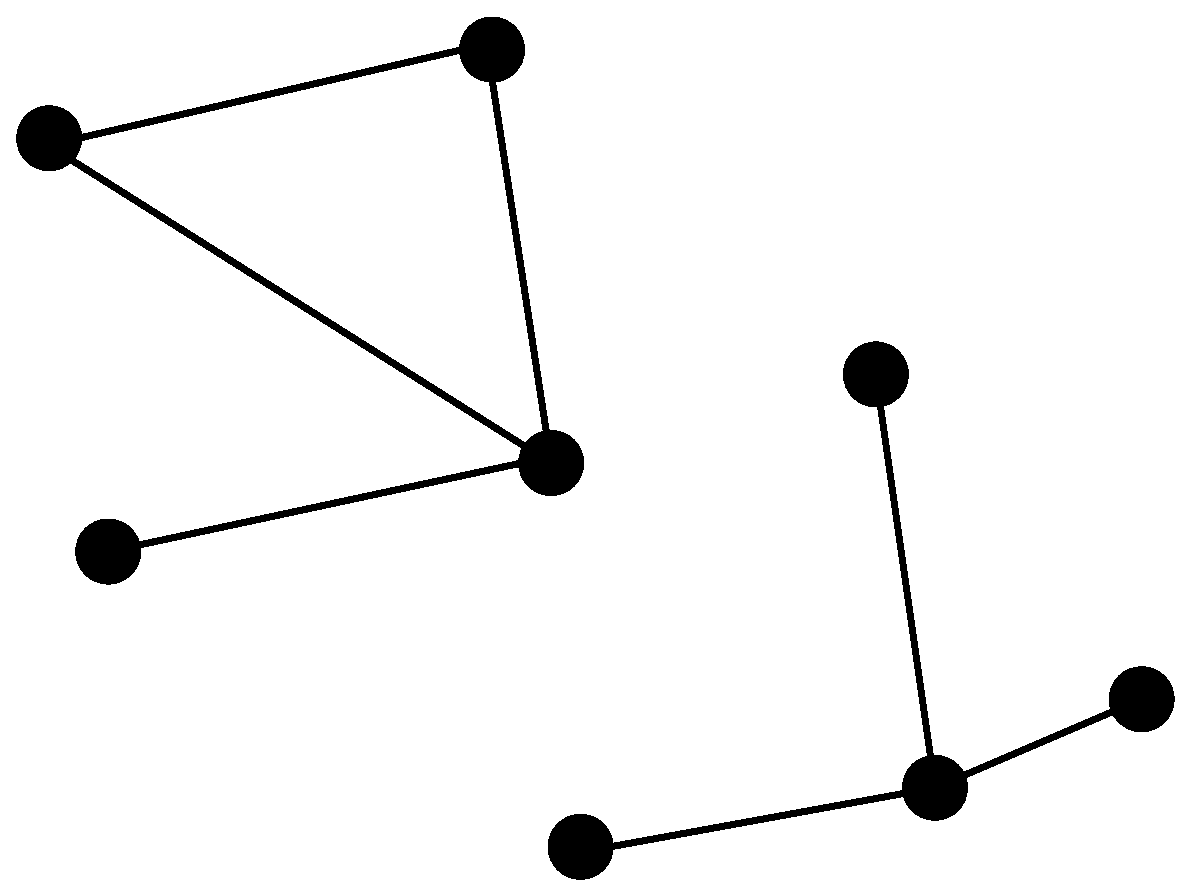
\includegraphics[width=\linewidth]{img/simple_two_island_graph.eps}
  \caption{Graph with 8 nodes and 7 branches. The graph contains two islands.}
  \label{fig:simple_two_island_graph}
\end{marginfigure}



\section{n-phase modelling}

The electrical grid calculations are mostly done in what is called \textit{positive sequence equivalent} (a single phase equivalent of a three-phase grid) In practice the positive sequence equivalent is applied to branches with one, two or three phases, this simplifies the modelling, but makes the realistic analysis of the grid much harder since the phases imbalance has been neglected.

In this book, three-phase models will be presented, but the calculations will be done on phase-by-phase basis. This is possible using the models presented by Vieira, Freitas and Morelato \cite{vieira2004phase}. In their work, the authors pick the diagonal of the elements admittance matrices to form single-phase grids, that are simulated independently. The magnetic coupling effects are included in the single-phase admittance matrices as shunt elements. This allows a very flexible model of the grid while retaining the calculation accuracy of a full-blown n-phase admittance matrix.

So, because of the latter, the models will be introduced in three-phases and whenever needed in positive sequence equivalents, but the numerical methods will consider only one phase at the time. In practice we will solve one numerical problem per phase. To simulate n phases, we will perform n numerical simulations, merging the results back into n-phase structures.

\begin{figure}
  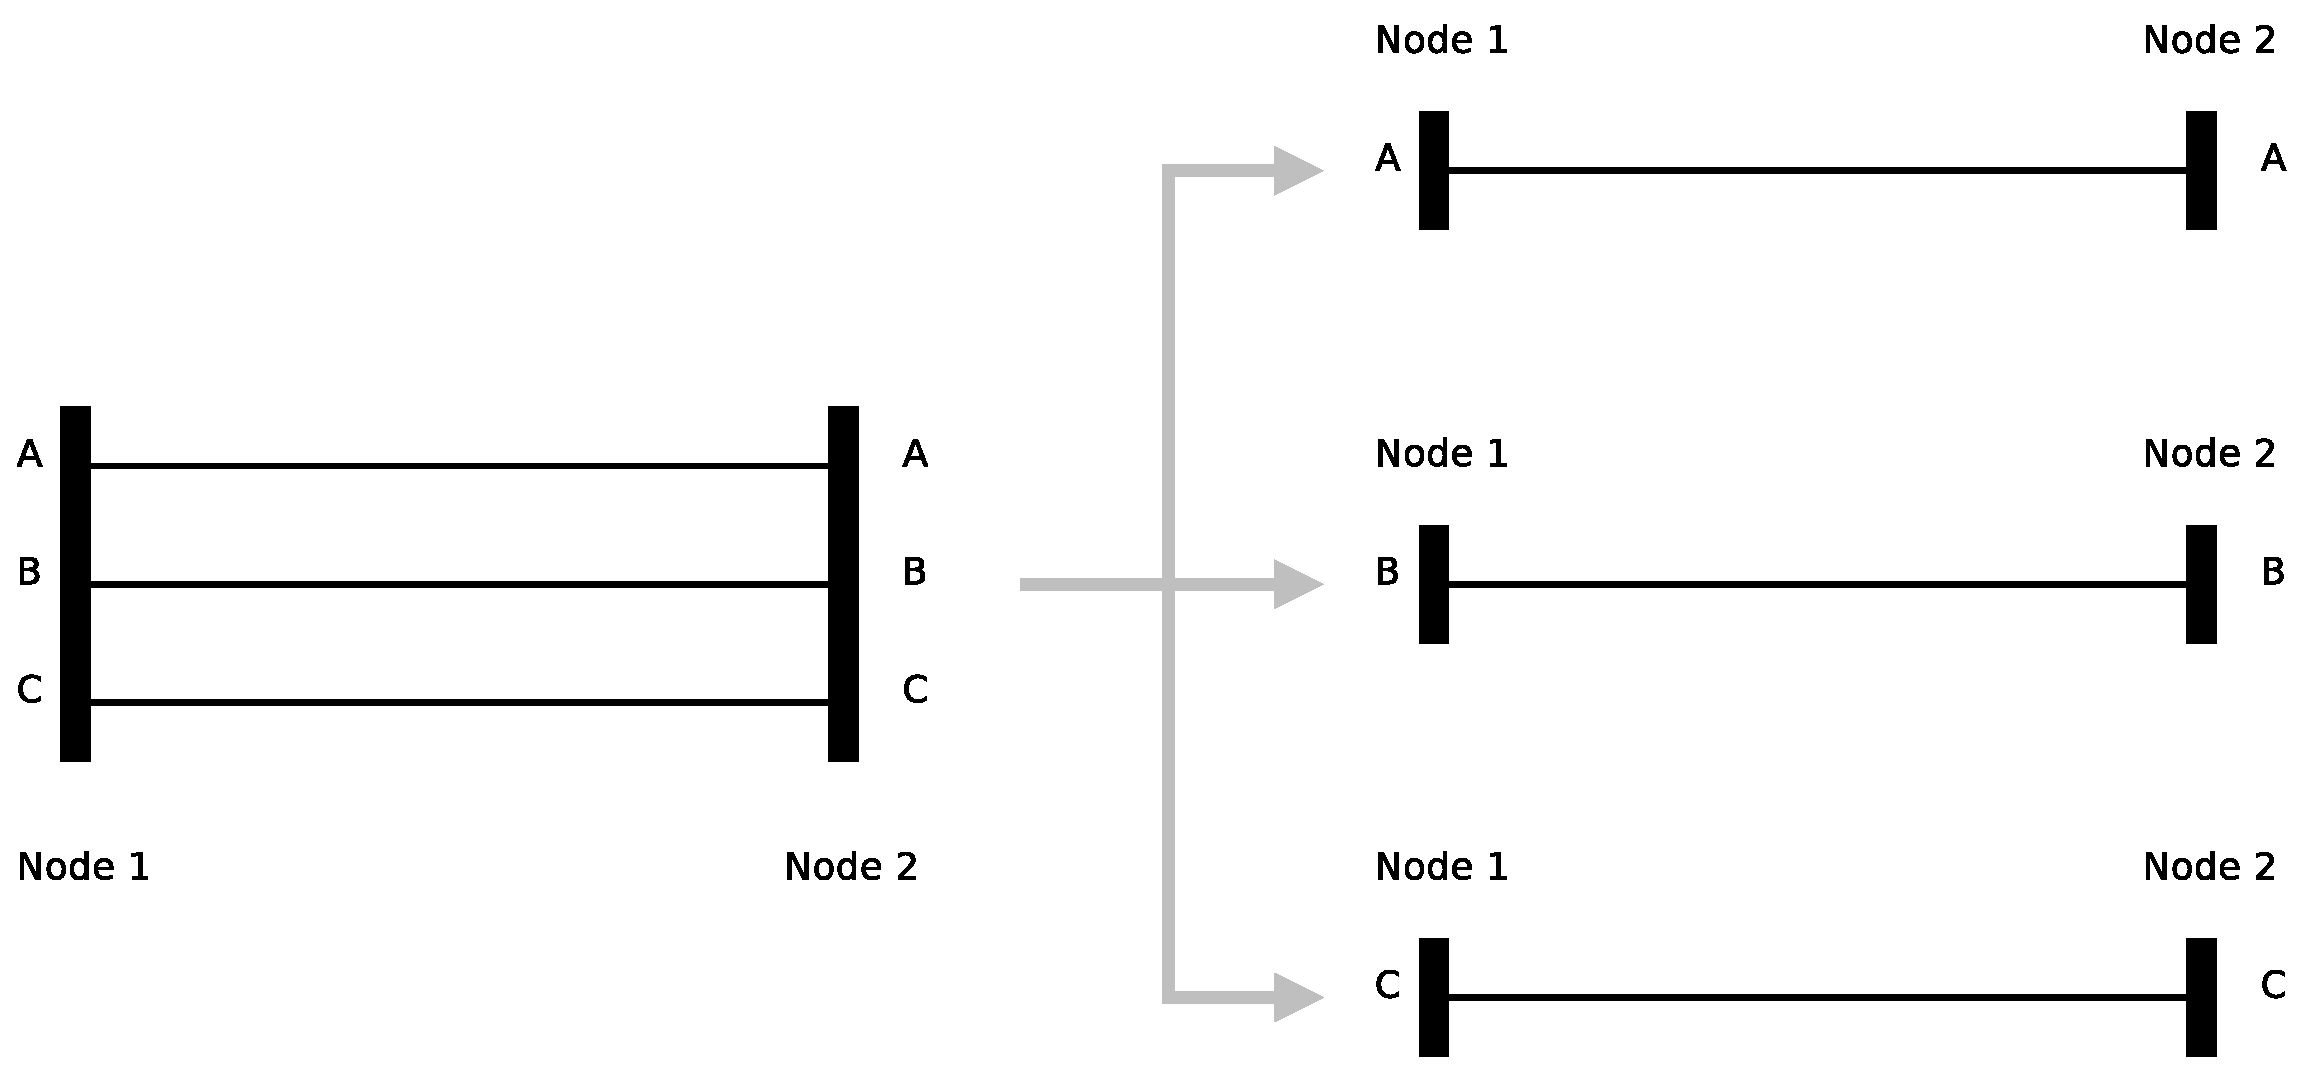
\includegraphics[width=\linewidth]{img/3p_to_1p.eps}
  \caption{Two node system in 3 phases, split into three systems of two nodes each.}
  \label{fig:3p_to_1p}
\end{figure}

Further details about how to decouple the three-phase impedance matrices into three single phase impedances are presented in the section \ref{sec:decoupling_branch}.

%-------------------------------------------------------------------------------
%	CHAPTER Magnitudes and units
%-------------------------------------------------------------------------------
\chapter{Magnitudes and units}

As the electric energy is mostly distributed in alternating current, electrical magnitudes are waves that vary their polarity (positive and negative value) and amplitude in time. because of this, the electrical magnitudes are expressed by complex numbers to denote the position of the value in the two-dimensional plane amplitude-time. 

\begin{marginfigure}
  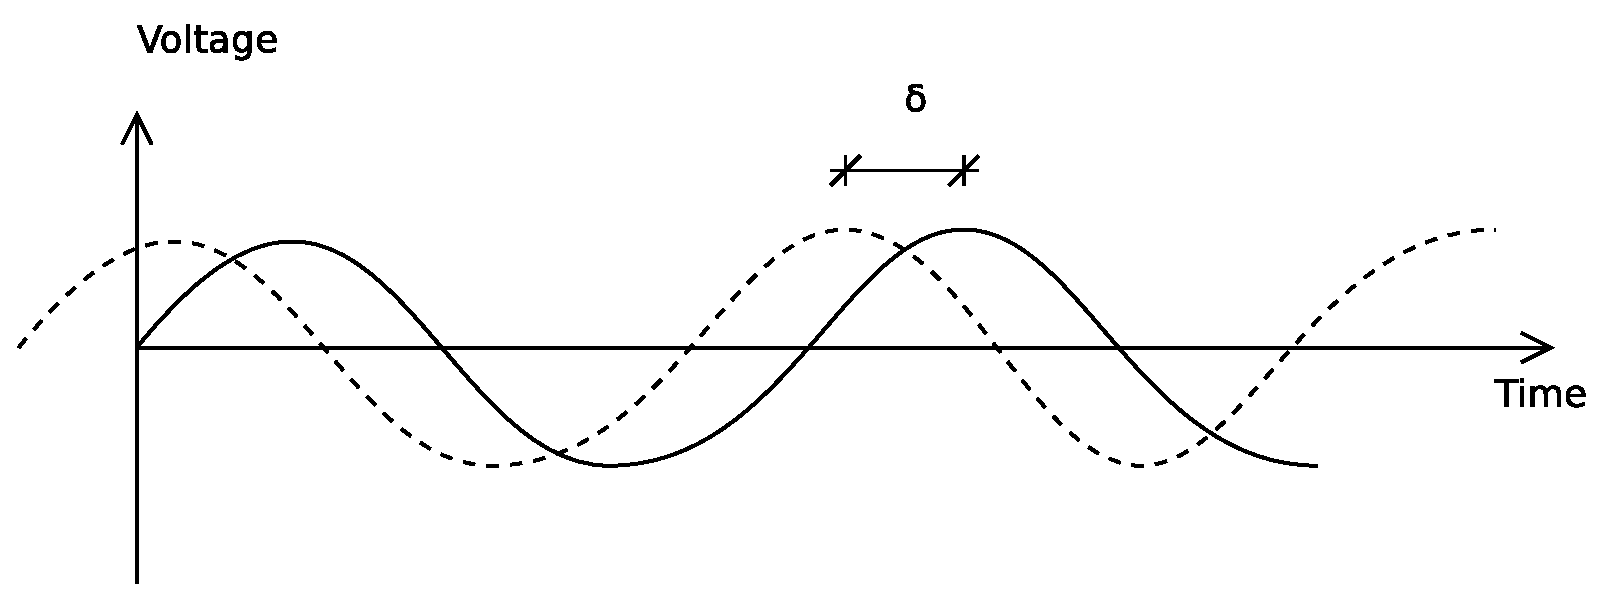
\includegraphics[width=\linewidth]{img/VoltageDelay.eps}
  \caption{Voltage delay.}
  \label{fig:vdelay}
\end{marginfigure}


The units in electrical grid modelling are represented in the tables \ref{units_table} and \ref{real_imaginary_table}.


\begin{table}[h]\index{typefaces!sizes}
\begin{center}
\footnotesize
\begin{tabular}{lll}
\toprule
Magnitude & Unit & Recommended user input unit\\
\midrule
Voltage & $V$ (Volt) & $kV$ (kilo-Volt)\\
Current & $A$ (Ampere) & $kA$ (kilo-Ampere)\\
Power & $VA$ (Volt-Ampere) & $MVA$ (Mega-Volt-Ampere)\\
Active power & $W$ (Watt) & $MW$ (Mega-Watt)\\
Reactive power & $VAr$ (Volt-Ampere-reactive) & $MVAr$ (Mega-Volt-Ampere-reactive)\\
Impedance & $\Omega$ (Ohm) & $\Omega$ (Ohm) or per-unit\\
Admittance & $S$ (Siemens) &  $S$ (Siemens) or per-unit\\
\bottomrule
\end{tabular}
\end{center}
  \caption{Electrical magnitudes and their units.}
  \label{units_table}
\end{table}


\begin{marginfigure}
  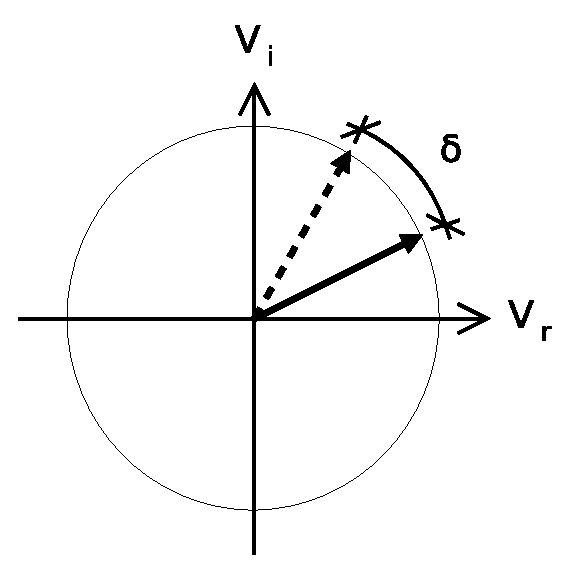
\includegraphics[width=0.5\linewidth]{img/VoltagePhasors.eps}
  \caption{Voltage delay in phasor representation in the complex plane.}
  \label{fig:vphasors}
\end{marginfigure}


The figure \ref{fig:vdelay} shows two voltage waves. The one represented with a dotted line is delayed an angle $\delta$ with respect to the reference voltage wave represented by the plain black line. Since both waves are periodical, both can be represented as "phasors" or vectors indicating the magnitude's value and angle in the complex rectangular plane as depicted in the figure \ref{fig:vphasors}. Figures \ref{fig:vdelay} and \ref{fig:vphasors} are equivalent representations.


\begin{table}[h]\index{typefaces!sizes}
\begin{center}
\footnotesize
\begin{tabular}{llll}
\toprule
Magnitude & Real part & Imaginary part & Relation\\
\midrule
$S$ (Power) & $P$ (Active power) & $Q$ (Reactive power) & $S=P +jQ$\\
$V$ (Voltage) & $V_r$ (Real voltage) & $V_i$ (Imaginary voltage) & $V=V_r +jV_i$\\
Expressed as  &  &  & \\
 & $V_m$ (Voltage module) &  & \\
 & $\delta$ (Voltage angle) &  & $V = V_m \cdot e^\delta$\\
  &  &  & \\
$I$ (Current) & $I_r$ (Real current) & $I_i$ (Imaginary current) & $I=I_r +jI_i$\\
$Z$ (Impedance) & $R$ (Resistance) & $X$ (Inductance) & $Z=R +jX$\\
$Y$ (Admittance) & $G$ (Conductance) & $B$ (Susceptance) & $Y=G +jB$\\
\bottomrule
\end{tabular}
\end{center}
  \caption{Magnitudes and their real and imaginary complex components.}
  \label{real_imaginary_table}
\end{table}






\section{Components connection and their conversions}

Let us assume a three-phase grid. The phases of the grid are denoted by the names of $A$, $B$ and $C$. There are two main connection types that arise: Wye (like the letter "y") and Delta.

The wye and delta connections provide the ground to introduce the \textit{phase} and \textit{line} voltages. The phase to neutral voltage is called \textit{phase voltage}, those are $V_A$, $V_B$ and $V_C$. The phase to phase voltage is called \textit{line voltage}, those are $V_{AB}$, $V_{AC}$ and $V_{BC}$.

\paragraph{The delta connection} is depicted in the figure \ref{fig:delta}. The delta connection has no neutral.

\paragraph{The wye connection} is depicted in the figure \ref{fig:star}. The star connection does have neutral ($N$). The wye connection is also known as star connection.

\begin{marginfigure}
  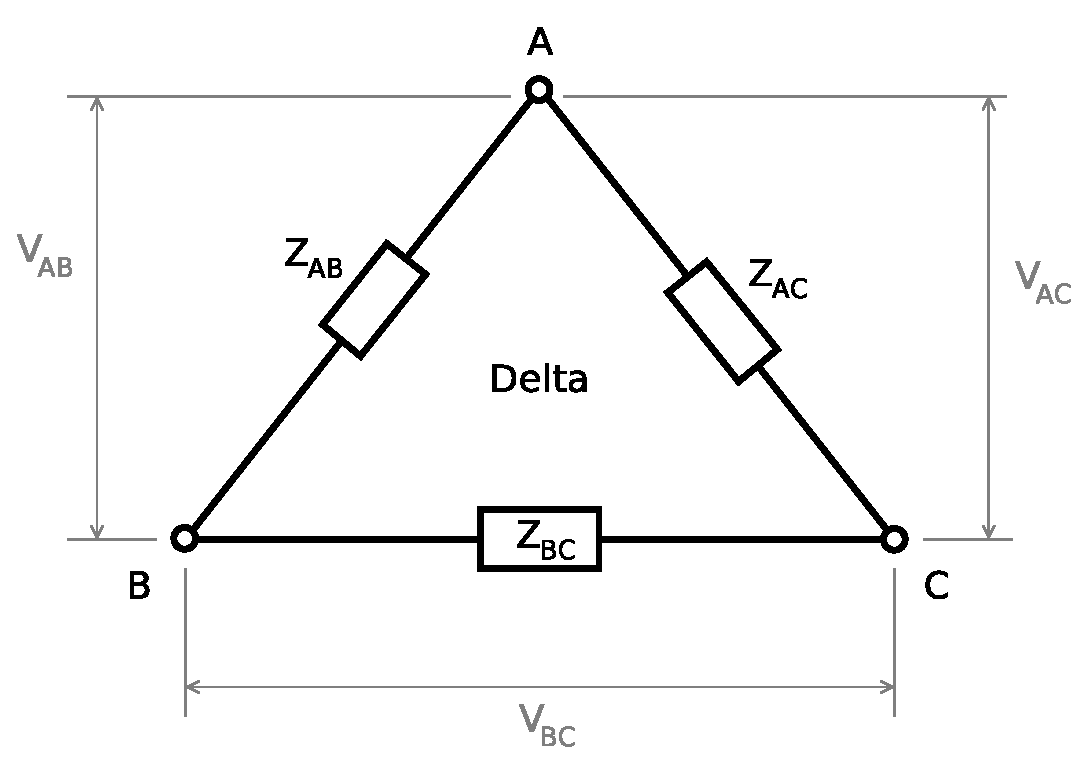
\includegraphics[width=0.9\linewidth]{img/Delta.eps}
  \caption{Delta connection scheme.}
  \label{fig:delta}
\end{marginfigure}

\begin{marginfigure}
  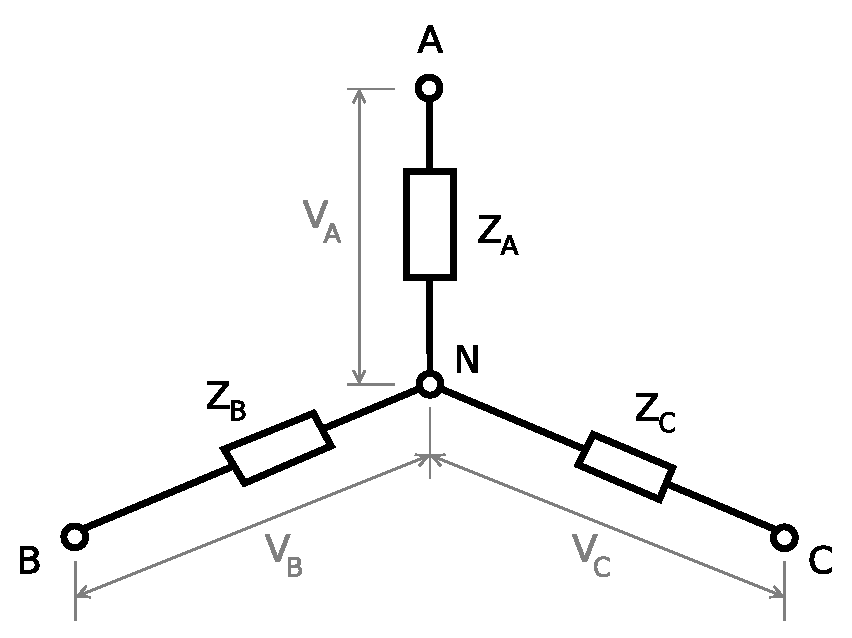
\includegraphics[width=0.9\linewidth]{img/Star.eps}
  \caption{Wye connection scheme.}
  \label{fig:star}
\end{marginfigure}

\paragraph{Delta to Wye ($\Delta \rightarrow Y$)} The transformation of a three phase connected shunt element in Delta to it's Wye equivalent is:

\begin{equation}
Elm_{Wye} = D \times Elm_{Delta}
\end{equation}

Where $D$ is:

\begin{equation}
D = \left[ \begin{array}{ccc}
1 & -1 & 0 \\
0 & 1 & -1 \\
-1 & 0 & 1
\end{array} \right]
\end{equation}

For instance, considering the impedances transformation from figures \ref{fig:delta} and \ref{fig:star}:

\begin{equation}
\left[ \begin{array}{c}
Z_A \\
Z_B \\
Z_C
\end{array} \right] = \left[ \begin{array}{ccc}
1 & -1 & 0 \\
0 & 1 & -1 \\
-1 & 0 & 1
\end{array} \right] \times \left[ \begin{array}{c}
Z_{AB} \\
Z_{AC} \\
Z_{BC}
\end{array} \right]
\end{equation}

\paragraph{Wye to Delta ($Y\rightarrow \Delta$)} The transformation of a three phase connected shunt element in Wye to it's Delta equivalent is:

\begin{equation}
Elm_{Delta} = D^{-1} \times Elm_{Wye}
\end{equation}

Where $D^{-1}$ is:

\begin{equation}
D^{-1} = \frac{1}{3} \left[ \begin{array}{ccc}
1 & 0 & -1 \\
-1 & 1 & 0 \\
0 & -1 & 1
\end{array} \right]
\end{equation}

For instance, considering the impedances transformation from figures \ref{fig:delta} and \ref{fig:star}:

\begin{equation}
\left[ \begin{array}{c}
Z_{AB} \\
Z_{AC} \\
Z_{BC}
\end{array} \right] = \frac{1}{3} \left[ \begin{array}{ccc}
1 & 0 & -1 \\
-1 & 1 & 0 \\
0 & -1 & 1
\end{array} \right] \times \left[ \begin{array}{c}
Z_A \\
Z_B \\
Z_C
\end{array} \right]
\end{equation}




\section{Per unit system}

In an electrical grid there are multiple levels of voltage. This situation introduces discontinuities in the numerical methods used to solve power flows and state estimations among others, producing an unstable convergence behaviour. To avoid this, the per unit system is introduced. A side effect of the per unit representation is to have a very convenient way of visualizing the grid magnitudes, all referenced to their base. In the per unit system, all the voltages are expressed in terms of their nominal value. In this case, all the grid voltage values are around one. For instance, a voltage value of 0.98 means that the voltage is 98 \% of the nominal voltage value at that point.

For most exchange formats in computer programs, the element's magnitudes are expressed with a mix of actual units and per unit values. Regardless of this, a practical way of converting any electrical magnitude to its per unit equivalent is presented.

First, we must choose an arbitrary value of power base conversion. This value can be seen as the grid's nominal power, even though that concept is not related to any physical quantity, but it is rather a numerical artifice. 

\marginnote{ The base power is most commonly chosen to be $S_{Base} = 100 MVA$.}




\bigskip
\begin{table}[h!]\index{typefaces!sizes}
\begin{center}
\footnotesize
\begin{tabular}{lll}
\toprule
Magnitude &  Base\\
\midrule
$V$ (Voltage) & $V_{Base}$: terminal's nominal voltage. \\
$S$ (Power) & $S_{Base}$: Arbitrary value, usually 10 MVA. \\
$I$ (Current) & $I_{Base} = S_{Base} / Vline_{Base} = S_{Base} / (V_{Base} \cdot \sqrt{3})$ \\
$Z$ (Impedance) & $Z_{Base} = V_{Base}^2 / S_{Base}$ \\
$Y$ (Admittance) & $Y_{Base} = 1 / Z_{Base}$ \\
\bottomrule
\end{tabular}
\end{center}
  \caption{Electrical magnitudes and their per unit base.}
  \label{magnitudes_and_their_base}
\end{table}


\section{Sequence components simplification}

Charles L. Fortescue presented in 1918 his famous article \cite{fortescue1918method} in which he describes how to represent a three-phase element in the so-called \textit{sequence components}.

The main use of this technique is to reduce the amount of impedances needed to represent a line or transformer from usually nine, to three (or even two) if the element is considered to be balanced. An element is considered balance if the impedance in all it's phases is equal and the phase-to-phase coupling impedances are also equal. This is an assumption that is commonly made for transmission grids (very high voltage) and distribution grids in high voltage. This advance allowed the popularization of the single-line diagrams in which every line represents a  a number of wires transmitting power in a balanced scheme.

Fortesue defined a transformation matrix $A_s$ and it's inverse as:

\begin{equation}
A_s = \left[ \begin{array}{ccc}
1 & 1 & 1 \\
1 & a^2 & a \\
1 & a & a^2
\end{array} \right]
\end{equation}

\begin{equation}
A_s^{-1} = \frac{1}{3}\left[ \begin{array}{ccc}
1 & 1 & 1 \\
1 & a & a^2 \\
1 & a^2 & a
\end{array} \right]
\end{equation}

Where $a$ is the transformation eigenvector:
\begin{equation}
a = 1^{120_{deg}} = 1 \cdot e^{j \frac{2}{3}\pi} = 1 \cdot cos\left(\frac{2}{3}\pi\right) + 1j \cdot sin\left(\frac{2}{3}\pi\right)
\end{equation}

\begin{equation}
a^2 = 1^{-120_{deg}} = 1 \cdot e^{-j \frac{2}{3}\pi} = 1 \cdot cos\left(\frac{2}{3}\pi\right) - 1j \cdot sin\left(\frac{2}{3}\pi\right)
\end{equation}


Then, any 3x3 impedance matrix representing the rectangular ABC three-phase impedance of an element (line, transformer, capacitor, etc.) can be transformed to a sequence equivalent using the formula:

\begin{equation}
Z_{seq} = A_s^{-1} \times Z_{ABC} \times A_s
\label{fortescue_transformation}
\end{equation}


\paragraph{Example}

Consider the following impedance matrix of a three-phase line. Example from \cite{kersting2012distribution}.

$$
Z_{ABC} = \left[ \begin{array}{ccc}
0.4576 + j 1.0780 & 0.1560 + j0 .5017 & 0.1535 + j 0.3849 \\
0.1560 + j 0.5017 & 0.4666 + j 1.0482 & 0.1580 + j 0.4236 \\ 
0.1535 + j 0.3849 & 0.1580 + j 0.4236 & 0.4615 + j 1.0651
\end{array} \right]
$$

Using equation \ref{fortescue_transformation}, we obtain the sequence impedance matrix:
$$
Z_{seq} = \left[ \begin{array}{ccc}
0.7735 + j 1.9373  & 0.0256 + j 0.0115 & – 0.0321 + j 0.0159 \\
-0.0321 + j 0.0159 & 0.3061 + j 0.6270 & – 0.0723  –  j 0.0060 \\ 
0.0256  +  j 0.0115 & -0.0723  –  j 0.0059 & 0.3061  +  j 0.6270
\end{array} \right]
$$

For the sequence matrix, the non diagonal elements are neglected. Using only the three diagonal elements as:

$$
\begin{array}{c}
Z_0 = 0.7735 + j 1.9373 \\
Z_1 = 0.3061 + j 0.6270 \\
Z_2 = 0.3061  +  j 0.6270
\end{array}
$$

Observe that $Z_1$ and $Z_2$ are identical (with the shown numerical precision). It is very common in utilities to store only $Z_0$ and $Z_1$ to define a line. The balanced element assumption is very common and should be carefully used.

\section{Building $Z_{ABC}$ from the sequence components}

Once the complete 3x3 impedance matrix has been reduced to the sequence components and only those have been stored in the utility database, the obtaining of the full 3x3 matrix might be necessary to perform unbalanced calculations. Of course we will not be able to obtain the exact original $Z_{ABC}$ from the reduced sequence components, but the approximation is fair.

The approximated full impedance matrix is obtained from the sequence components as:

\begin{equation}
Z_{ABC_{approx}} = \frac{1}{3}\left[ \begin{array}{ccc}
2Z_1 + Z_0 & Z_0 - Z_1 & Z_0 - Z_1 \\
Z_0 - Z_1 & 2Z_1 + Z_0 & Z_0 - Z_1 \\ 
Z_0 - Z_1 & Z_0 - Z_1 & 2Z_1 + Z_0
\end{array} \right]
\end{equation}

\paragraph{Example}

We need to compute two values, before assembling the 3x3 matrix:

$$
\frac{1}{3}(2 \cdot Z_1 + Z_0) = \frac{1}{3} (2\cdot(0.3061 + j 0.6270) + (0.7735 + j 1.9373)) = 0.4619 + j1.0638
$$

$$
\frac{1}{3} (Z_0 - Z_1) = \frac{1}{3}((0.7735 + j 1.9373) - (0.3061 + j 0.6270)) = 0.1558 + j0.4368
$$

The the approximated impedance matrix is:

$$
Z_{ABC_{approx}} = \left[ \begin{array}{ccc}
0.4619 + j1.0638 & 0.1558 + j0.4368 & 0.1558 + j0.4368 \\
0.1558 + j0.4368 & 0.4619 + j1.0638 & 0.1558 + j0.4368 \\ 
0.1558 + j0.4368 & 0.1558 + j0.4368 & 0.4619 + j1.0638
\end{array} \right]
$$

We observe that the calculation outcome is a fair approximation of the original $Z_{ABC}$ and that the approximated matrix is symmetric, matching the balanced assumption, which the original impedance matrix did not fully comply with. Therefore, is the original $Z_{ABC}$ was reduced assuming a balanced impedance distribution when that was not the case, if we build the approximated matrix, we will never know if it represents the reality.





%-------------------------------------------------------------------------------
%	CHAPTER The branch element
%-------------------------------------------------------------------------------

\chapter{The branch element} 
\label{ch:branch}

To the effect of most calculations run in operation of a electrical system, the lines, transformers, and any other element that connects two nodes are represented by the so-called $\Pi$ model.


\section{$\Pi$ Model}

\marginnote{In the case of lines, the series admittance $\textbf{Y}_{serie}$ is computed as the inverse of $\textbf{Z}_{ABC}$. From the line's calculation it is obtained the series impedance matrix $\textbf{Z}_{ABC}$ and the shunt admittance matrix $\textbf{Y}_{sh}$. }

The pi model is composed by a series admittance  $\textbf{Y}_{serie}$ and a shunt admittance $\textbf{Y}_{sh}$ divided in two. The shunt admittances are connected at the sending and receiving terminals (primary and secondary). To accommodate the possibility of regulating the voltage at the sending and/or receiving terminals, two per-unit transformers are included as well. The per unit transformers are modelled with the \textit{tap ratio} parameters $\alpha$ and $\beta$.


\begin{center}
	\begin{figure*}[h]
		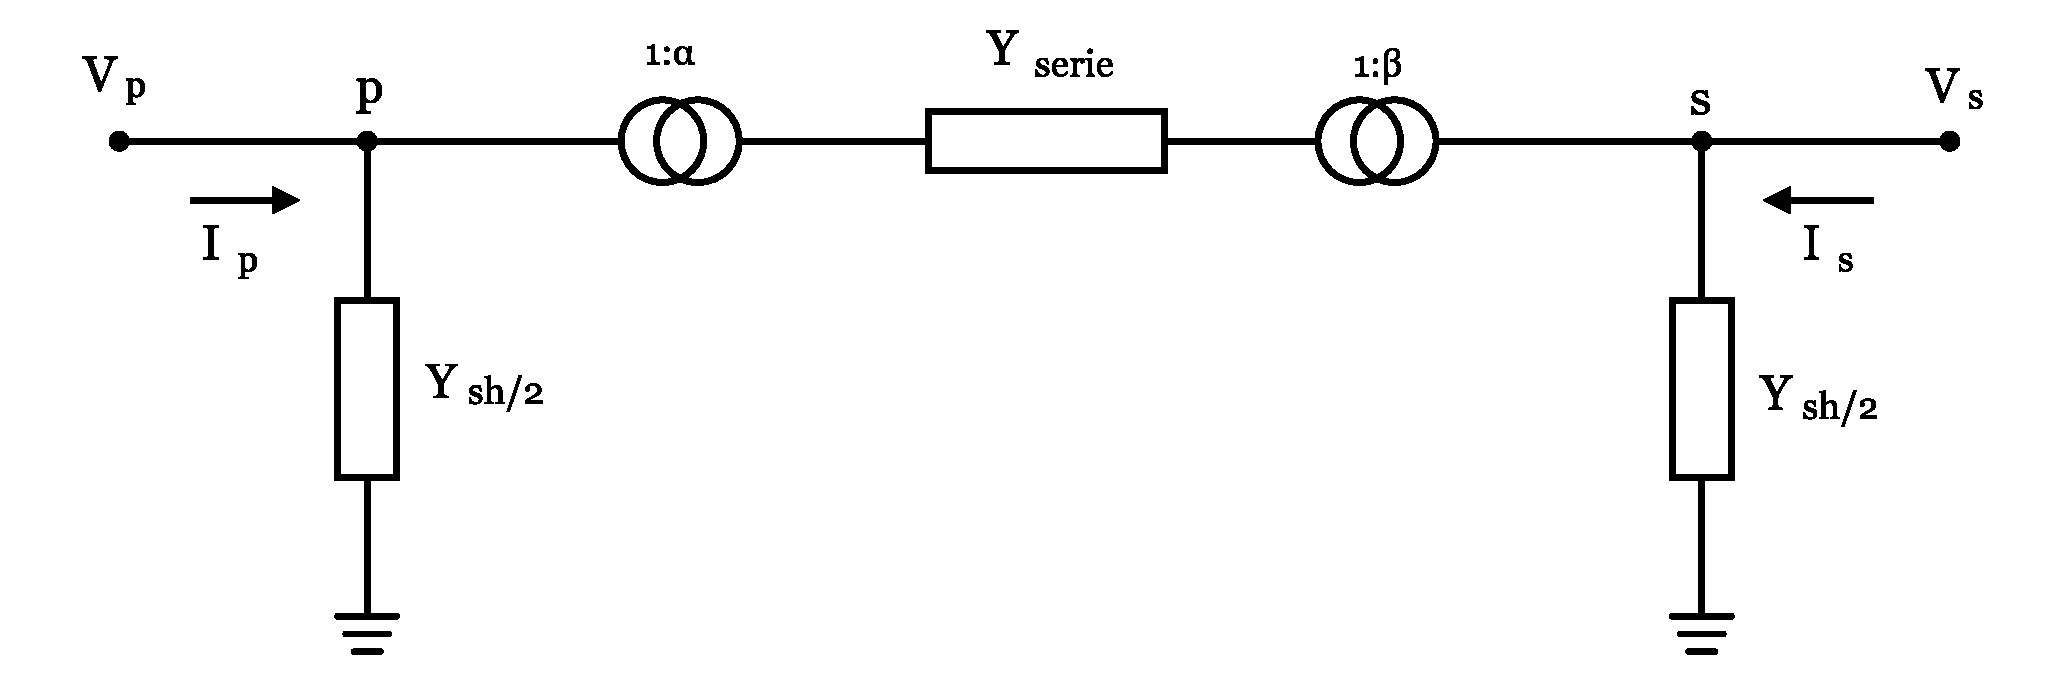
\includegraphics[width=0.6\linewidth]{img/Branch.eps}
		\caption{General branch model.}
		\label{pi_model}
	\end{figure*}
\end{center}

The generalized admittance matrix that corresponds to the $\Pi$ model is:
\begin{equation}
\left[\begin{array}{c}
\textbf{I}_p \\
\textbf{I}_s
\end{array}\right] = \left[\begin{array}{cc}
\textbf{Y}_{pp} & \textbf{Y}_{ps} \\
\textbf{Y}_{sp} & \textbf{Y}_{ss}
\end{array}\right] \times \left[\begin{array}{c}
\textbf{V}_p \\
\textbf{V}_s
\end{array}\right]
\label{pi_main_formula}
\end{equation}

Where:

\begin{table}[h!]
\begin{center}
\begin{tabular}{cccc}
\toprule

$\textbf{Y}_{pp}$ &  $\textbf{Y}_{ps}$ & $\textbf{Y}_{sp}$ & $\textbf{Y}_{ss}$\\

\midrule

$\frac{\textbf{Y}_{series} + \frac{\textbf{Y}_{sh}}{2}}{\alpha^2}$ &  $\frac{-\textbf{Y}_{series}}{\alpha\beta}$ & $\frac{-\textbf{Y}_{series}}{\alpha\beta}$ & $\frac{\textbf{Y}_{series} + \frac{\textbf{Y}_{sh}}{2}}{\beta^2}$\\

\bottomrule
\end{tabular}
\end{center}
  \caption{Equations of the generalized $\Pi$ model.}
  \label{pi_model_equations}
\end{table}

The formula \ref{pi_main_formula} will be used to compute the network admittance matrices.


\subsection{Positive sequence model}

A positive sequence model of the $\Pi$ branch model is very useful. The formulation of the admittance matrix of the branch is close to the one presented but since it is not in three-phase, varies a bit.

\begin{center}
	\begin{figure*}[h]
		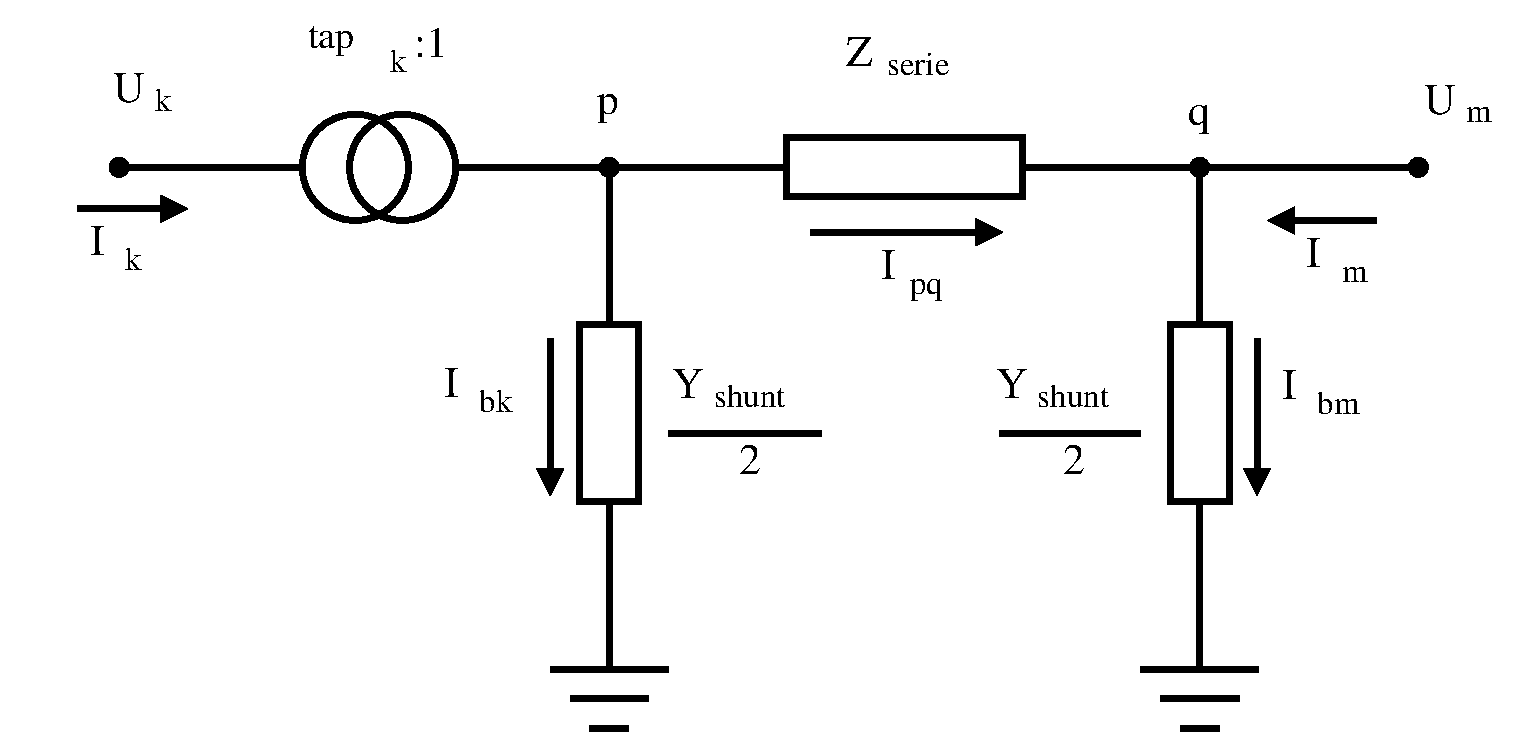
\includegraphics[width=0.5\linewidth]{img/pi-trafo.eps}
		\caption{General positive sequence branch model.}
		\label{pi_model_ps}
	\end{figure*}
\end{center}

\begin{itemize}
	\item $z_{series}$: Magnetizing impedance or simply series impedance. It is given in p.u.
	\item $y_{shunt}$: Leakage impedance or simply shunt impedance. It is given in p.u.
	\item $tap\_module$: Module of the tap changer. It is a magnitude around 1.
	\item $tap\_angle$: Angle of the tap changer. Angle in radians.\newline
\end{itemize}


%tap = self.tap_module * exp(-1j * self.angle)

In order to apply the effect of a branch to the admittance matrices, first we compute the complex tap value.
$$tap = tap\_module \cdot e^{-j \cdot tap\_angle}$$  

Then we compose the equivalent series and shunt admittance values of the branch. Both values are complex.
%Ys = 1 / self.z_series
$$Y_s = \frac{1}{z_{series}}$$
%Ysh = self.y_shunt / 2
$$Y_{sh} = \frac{y_{shunt}}{2}$$

\begin{itemize}
	\item $z_{series}$: Series impedance of the branch composed by the line resistance and its inductance. $z_{series}=r + jl$
	
	\item $y_{shunt}$: Shunt admittance of the line composed by the conductance and the susceptance. $y_{shunt}=c+jb$\newline
\end{itemize}



The general branch model is represented by a $2 \times 2$ matrix.
%\vspace{0.5cm}
$$
Y_{branch}=\left[ \begin{array}{ccc}
Y_{ff} & Y_{ft} \\
Y_{tf} & Y_{tt} \end{array} \right]
$$
%\vspace{0.5cm}
In this matrix, the elements are the following:

%Yff = Ytt / (tap * conj(tap))
%Yft = - Ys / conj(tap)
%Ytf = - Ys / tap
%Ytt = Ys + Ysh

$$Y_{ff} = \frac{Y_s + Y_{sh}}{tap \cdot conj(tap)}  $$
$$Y_{ft} = - Y_s / conj(tap)$$
$$Y_{tf} = - Y_s / tap$$
$$Y_{tt} = Y_s + Y_{sh}$$



\section{Line}

The line element, utilizes the branch model as it has been formulated, only that the use of the tap ratio relations $\alpha$ and $\beta$ is not necessary.


\subsection{Overhead lines}


\subsection{Underground cables}


\paragraph{Example}

Let's assume that we have already computed the series impedance and the shunt admittance of a three-phase line. The nominal voltage at the line terminals is $66kV$ and we choose the base power to be $S_{base}=100MVA$.

$$
Z_{ABC} = \left[ \begin{array}{ccc}
0.4576 + j 1.0780 & 0.1560 + j0 .5017 & 0.1535 + j 0.3849 \\
0.1560 + j 0.5017 & 0.4666 + j 1.0482 & 0.1580 + j 0.4236 \\ 
0.1535 + j 0.3849 & 0.1580 + j 0.4236 & 0.4615 + j 1.0651
\end{array} \right] \Omega
$$

$$
Y_{sh} = \left[ \begin{array}{ccc}
j5.6712 & -j1.8362 & -j0.7034 \\
-j1.8362 & j5.9774 & -j1.1690 \\ 
-j0.7034 & -j1.1690 & j5.3911
\end{array} \right] \cdot 10^{-6}  S
$$

The first thing we need to do is to compute the base magnitudes:

$$
Z_{base} = \frac{100 MVA}{(66kV)^2} = 0.022956841 \quad \Omega
$$

$$
Y_{base} = \frac{1}{Z_{base}} = 43.56 \quad S
$$

Then we must obtain the line series admittance matrix $Y_{series}$ by inverting the 3x3 matrix $Z_{ABC}$. The we divide the resulting matrix by $Y_{base}$. Analogously we can invert the per unit impedance matrix:

$$
Y_{series} = \left(\frac{Z_{ABC}}{Z_{base}}\right)^{-1} \quad p.u.
$$

$$
Y_{series} = \left[ \begin{array}{ccc}
0.0112-j0.0232  & -0.0054+j0.008   & -0.0020+j0.0052 \\ -0.0054+j0.008  &  0.0125-j0.024 & -0.0033+j0.0063 \\ -0.0020+j0.0052 &  -0.0033+j0.0063 & 0.0100-j0.0224
\end{array} \right]\quad  p.u.
$$

Dividing the shunt admittance by the base admittance we obtain the per unit shunt admittance:

$$
Y_{sh} = \left[ \begin{array}{ccc}
j13.0193 & -j4.2153 &  -j1.6148 \\
-j4.2153 & j13.7222 & -j2.6837 \\ 
-j1.6148 & -j2.6837 & j12.3763
\end{array} \right] \cdot 10^{-8}  \quad p.u.
$$

Now we need to find the branch model admittances $Y_{pp}$, $Y_{ps}$, $Y_{sp}$ and $Y_{ss}$.

$$
Y_{pp} = Y_{ss} = Y_{series} + Y_{sh}/2 = \left[ \begin{array}{ccc}
0.0112-j0.0232  & -0.0054+j0.008   & -0.0020+j0.0052 \\ -0.0054+j0.008  &  0.0125-j0.024 & -0.0033+j0.0063 \\ -0.0020+j0.0052 &  -0.0033+j0.0063 & 0.0100-j0.0224
\end{array} \right]\quad  p.u.
$$

$$
Y_{ps} = Y_{sp} = -Y_{series} = \left[ \begin{array}{ccc}
-0.0112+j0.0232  & 0.0054-j0.008   & 0.0020-j0.0052 \\  0.0054-j0.008  &  -0.0125+j0.024 & 0.0033-j0.0063 \\  0.0020-j0.0052 &  0.0033-j0.0063 & -0.0100+j0.0224
\end{array} \right]\quad  p.u.
$$

If we convert the three-phase matrices into positive sequence values we obtain:

$$
Y_{pp} = Y_{ss} = 0.0148 -j0.0296
$$

$$
Y_{ps} = Y_{sp} = -0.0148 +j0.0296
$$


$$
\left[\begin{array}{c}
I_p \\
I_s
\end{array}\right] = \left[\begin{array}{cc}
0.0148 -j0.0296 & -0.0148 +j0.0296\\
-0.0148 +j0.0296 & 0.0148 -j0.0296
\end{array}\right] \times \left[\begin{array}{c}
V_p \\
V_s
\end{array}\right]
$$



\newpage
\section{Transformer}

The transformer model implements the branch model as well, but the model admittances $Y_{pp}$, $Y_{ps}$, $Y_{sp}$ and $Y_{ss}$ vary depending on the connections types at the primary and at the secondary.

The most common transformer connections at the terminals are:

\begin{itemize}
\item Delta ($\Delta$)
\item Wye ($Y$)
\item Grounded Wye (the neutral is grounded) ($Yg$)
\end{itemize}



\begin{table}[h!]\index{typefaces!sizes}
\begin{center}
\begin{tabular}{ccccc}
\toprule
Primary & Secondary & $Y_{pp}$  & $Y_{ss}$ & $Y_{ps}$ and $Y_{sp}$\\
\midrule
 $Yg$ & $Yg$ 			& $\frac{1}{\alpha^2}Y_I$ 				& $\frac{1}{\beta^2}Y_I$ 		& $-\frac{1}{\alpha\beta}Y_I$\\
 $Yg$ & $Y$ 			& $\frac{1}{3\alpha^2}Y_{II}$			& $\frac{1}{3\beta^2}Y_{II}$	& $-\frac{1}{3\alpha\beta}Y_{II}$	\\
 $Yg$ & $\Delta$  		& $\frac{1}{\alpha^2}Y_I$ 				& $\frac{1}{\beta^2}Y_{II}$ 	& $\frac{1}{\alpha\beta}Y_{III}$	 \\
 $Y$ & $Yg$ 			& $\frac{1}{3\alpha^2}Y_{II}$			& $\frac{1}{3\beta^2}Y_{II}$	& $-\frac{1}{3\alpha\beta}Y_{II}$ \\
 $Y$ & $Y$  			& $\frac{1}{3\alpha^2}Y_{II}$			& $\frac{1}{\beta^2}Y_{II}$ 	& $\frac{1}{\alpha\beta}Y_{III}$	 \\
 $\Delta$ & $\Delta$ 	& $\frac{1}{\alpha^2}Y_{II}$			& $\frac{1}{\beta^2}Y_{II}$		& $-\frac{1}{\alpha\beta}Y_{II}$\\
 $\Delta$ & $Yg$ 		& $\frac{1}{\alpha^2}Y_{II}$			& $\frac{1}{\beta^2}Y_{I}$		& $\frac{1}{\alpha\beta}Y_{III}$\\
\bottomrule
\end{tabular}
\end{center}
  \caption{Three-phase transformer impedances of the branch model.}
  \label{transfoemer_impedances_table}
\end{table}

The table \ref{transfoemer_impedances_table} lays out the branch admittances for every pair of connections. The source for this model is the excellent book by J.Arrillaga\cite{arrillaga1990computer}.

\begin{equation}
Y_{I} = \left[ \begin{array}{ccc}
y_t & 0 &  0 \\
0 & y_t & 0 \\ 
0 & 0 & y_t
\end{array} \right] 
\end{equation}

\begin{equation}
Y_{II} = \left[ \begin{array}{ccc}
2y_t & -y_t &  -y_t \\
-y_t & 2y_t & -y_t \\  
-y_t & -y_t & 2y_t
\end{array} \right] 
\end{equation}

\begin{equation}
Y_{III} = \left[ \begin{array}{ccc}
-y_t & y_t &  0 \\
0 & -y_t & y_t \\ 
y_t & 0 & -y_t
\end{array} \right] \newline
\end{equation}


$y_t$ is the transformer winding per unit admittance. It is given in values per units from the transformer specifications sheet. Usually it is given either directly as magnetizing resistance $r_m$ and inductance $x_m$, in which case:

\begin{equation}
y_t = \frac{3}{r_l + jx_l}
\end{equation}

Or it is given as the "short circuit study" values. This is a more complete case.



\subsection{Transformer definition from the short circuit study}

In order to get the series impedance and shunt admittance of the transformer to match the branch model, it is advised to transform the specification sheet values of the device into the desired values. The values to take from the specifications sheet are: \newline
\begin{itemize}
	\item $S_n$: Nominal power in MVA.
	\item $U_{hv}$: Voltage at the high-voltage side in kV.
	\item $U_{lv}$: Voltage at the low-voltage side in kV.
	\item $U_{sc}$: Short circuit voltage in \%.
	\item $P_{cu}$: Copper losses in kW.
	\item $I_0$: No load current in \%.
	\item $GX_{hv1}$: Reactance contribution to the HV side. Value from 0 to 1.
	\item $GR_{hv1}$: Resistance contribution to the HV side Value from 0 to 1.\newline
\end{itemize}

Then, the series and shunt impedances are computed as follows:

\begin{multicols}{2}
Nominal impedance HV (Ohm): 
\begin{equation}
Zn_{hv} = U_{hv}^2 / S_n
\end{equation}


Nominal impedance LV (Ohm): 
\begin{equation}
Zn_{lv} = U_{lv}^2 / S_n
\end{equation}

Short circuit impedance (p.u.): 
\begin{equation}
z_{sc} = U_{sc} / 100
\end{equation}

Short circuit resistance (p.u.): 
\begin{equation}
r_{sc} = \frac{P_{cu} / 1000}{S_n}
\end{equation}

Short circuit reactance (p.u.):
\begin{equation}
x_{sc} = \sqrt{z_{sc}^2 - r_{sc} ^2}
\end{equation}


HV resistance (p.u.):
\begin{equation}
r_{cu,hv} = r_{sc} \cdot GR_{hv1}
\end{equation}

LV resistance (p.u.): 
\begin{equation}
r_{cu,lv} = r_{sc} \cdot (1 - GR_{hv1})
\end{equation}

HV shunt reactance (p.u.): 
\begin{equation}
xs_{hv} = x_{sc} \cdot GX_{hv1}
\end{equation}

LV shunt reactance (p.u.): 
\begin{equation}
xs_{lv} = x_{sc} \cdot (1 - GX_{hv1})
\end{equation}

Shunt resistance (p.u.): 
\begin{equation}
r_{fe} = \frac{Sn}{P_{fe} / 1000}
\end{equation}

Magnetization impedance (p.u.):
\begin{equation}
z_m = \frac{1}{I_0 / 100}
\end{equation}

Magnetization reactance (p.u.):
\begin{equation}
x_m = \frac{1}{\sqrt{\frac{1}{z_m^2} - \frac{1}{r_{fe}^2}}}
\end{equation}

If the content of the square root is negative, set the magnetization impedance to zero.\\


The final complex calculated parameters in per unit are:

Magnetizing impedance (or series impedance): 
\begin{equation}
z_{series} = Z_m = r_{sc} +j \cdot x_{sc}
\end{equation}

The series admittance is [p.u.]: 
\begin{equation}
y_{series} = \frac{1}{z_{series}}
\end{equation}

Leakage impedance (or shunt impedance): 
\begin{equation}
Z_l = r_{fe} + j \cdot x_{m}
\end{equation}

Shunt admittance [p.u.]: 
\begin{equation}
y_{shunt} = 1 / Z_l
\end{equation}


The series admittance for the three-phase model [p.u.]: 
\begin{equation}
y_{t} = \frac{3}{z_{series}}
\end{equation}
\end{multicols}

\marginnote{we divide the impedance by 3, to reflect the three phases.}


\paragraph{Example}

Let's consider a distribution transformer with the following nameplate characteristics:


\begin{multicols}{2}
\begin{itemize}
\item Primary connection: $\Delta$
\item Secondary connection: $Yg$
\item $S_n = 0.5 MVA$
\item $U_{hv} = 20  kV$
\item $U_{lv} = 0.4 kV$

\item $U_{sc} = 6  \%$
\item $p_{cu} = 6  kW$
\item $p_{fe} = 1.4 kW$
\item $I_0 = 0.28 \%$

\item $GR_{hv} = 0.5$
\item $GX_{hv} = 0.5$
\end{itemize}
\end{multicols}


First we obtain the impedance value, from the short circuit study:
\begin{multicols}{2}
$$Zn_{hv} =  800 \quad \Omega$$
$$Zn_{lv} =  0.3200 \quad \Omega$$
$$z_{sc} =  0.0600 \quad p.u.$$
$$r_{sc} =  0.0120 \quad p.u.$$
$$x_{sc} =  17.0103 \quad p.u.$$
$$r_{cu,hv} =  0.0060 \quad p.u.$$
$$r_{cu,lv} =  0.0060 \quad p.u.$$
$$x_{s,hv} =  8.5052 \quad p.u.$$
$$x_{s,lv} =  8.5052 \quad p.u.$$
$$r_{fe} =  357.1429 \quad p.u.$$
$$z_m =  357.1429 \quad p.u.$$
$$x_m =  24296003999.8084 \quad p.u.$$
$$z_{series} =  0.0120 + j17.0103 \quad p.u.$$
$$y_{series} =  0.0000 - j0.0588 \quad p.u.$$
$$y_{shunt} =  0.0000 - j0.0000 \quad p.u.$$
$$y_t =  0.0001 - j0.1764 \quad p.u.$$
\end{multicols}

Once the we have obtained the $y_t$ value, we start building the appropriate branch impedance matrices $Y_{pp}$, $Y_{ps}$, $Y_{sp}$ and $Y_{ss}$.
$$
Y_{I} = \left[\begin{array}{ccc}
0.0001 - j0.1764 & 0.0000 + j0.0000 & 0.0000 + j0.0000 \\
0.0000 + j0.0000 & 0.0001 - j0.1764 & 0.0000 + j0.0000 \\
0.0000 + j0.0000 & 0.0000 + j0.0000 & 0.0001 - j0.1764
\end{array} \right]
$$


$$
Y_{II} = \left[ \begin{array}{ccc}
0.0002 - j0.3527 & -0.0001 + j0.1764 & -0.0001 + j0.1764\\
-0.0001 + j0.1764 & 0.0002 - j0.3527 & -0.0001 + j0.1764\\
-0.0001 + j0.1764 & -0.0001 + j0.1764 & 0.0002 - j0.3527
\end{array} \right]
$$

$$
Y_{III} = \left[ \begin{array}{ccc}
-0.0001 + j0.1764 & 0.0001 - j0.1764 & 0.0000 + j0.0000\\
0.0000 + j0.0000 & -0.0001 + j0.1764 & 0.0001 - j0.1764\\
0.0001 - j0.1764 & 0.0000 + j0.0000 & -0.0001 + j0.1764
\end{array} \right]
$$


According to the transformer $\Delta \rightarrow Yg$ connection, we build the branch model admittances using the formulas for the table \ref{transfoemer_impedances_table}:

$$
Y_{pp} =\left[ \begin{array}{ccc}
0.0002 - j0.3527 & -0.0001 + j0.1764 & -0.0001 + j0.1764\\
-0.0001 + j0.1764 & 0.0002 - j0.3527 & -0.0001 + j0.1764\\
-0.0001 + j0.1764 & -0.0001 + j0.1764 & 0.0002 - j0.3527
\end{array} \right]
$$


$$
Y_{ss} =\left[ \begin{array}{ccc}
0.0001 - j0.1764 & 0.0000 + j0.0000 & 0.0000 + j0.0000\\
0.0000 + j0.0000 & 0.0001 - j0.1764 & 0.0000 + j0.0000\\
0.0000 + j0.0000 & 0.0000 + j0.0000 & 0.0001 - j0.1764
\end{array} \right]
$$


\marginnote{There is no computational need to assemble the 6x6 element impedance matrix in a computer program. The branch model matrices are added to the full circuit matrix instead.}

$Y_{ps} = Y_{sp} =$
$$
\left[ \begin{array}{ccc}
-0.0001 + j0.1764 & 0.0001 - j0.1764 & 0.0000 + j0.0000\\
0.0000 + j0.0000 & -0.0001 + j0.1764 & 0.0001 - j0.1764\\
0.0001 - j0.1764 & 0.0000 + j0.0000 & -0.0001 + j0.1764
\end{array} \right]
$$





\section{Voltage regulator}

Since all the electrical models are in per-unit values, the voltage regulator is modelled in the exact same way as a transformer.


\label{sec:decoupling_branch}
\section{Decoupling the three-phase model. Delta branch to Y branch transformation}

We have presented a three-phase branch model with 3x3 matrices. However we indicated at the beginning of this book that we would not perform the three-phase calculations using the coupled matrices (which would lead to larger linear systems to solve and the impossibility to solve multi-phase grids). This is why we are going to introduce a technique to decouple the phases while keeping the phase-phase influences (the non diagonal elements of the branch element matrix.)

\begin{figure}
	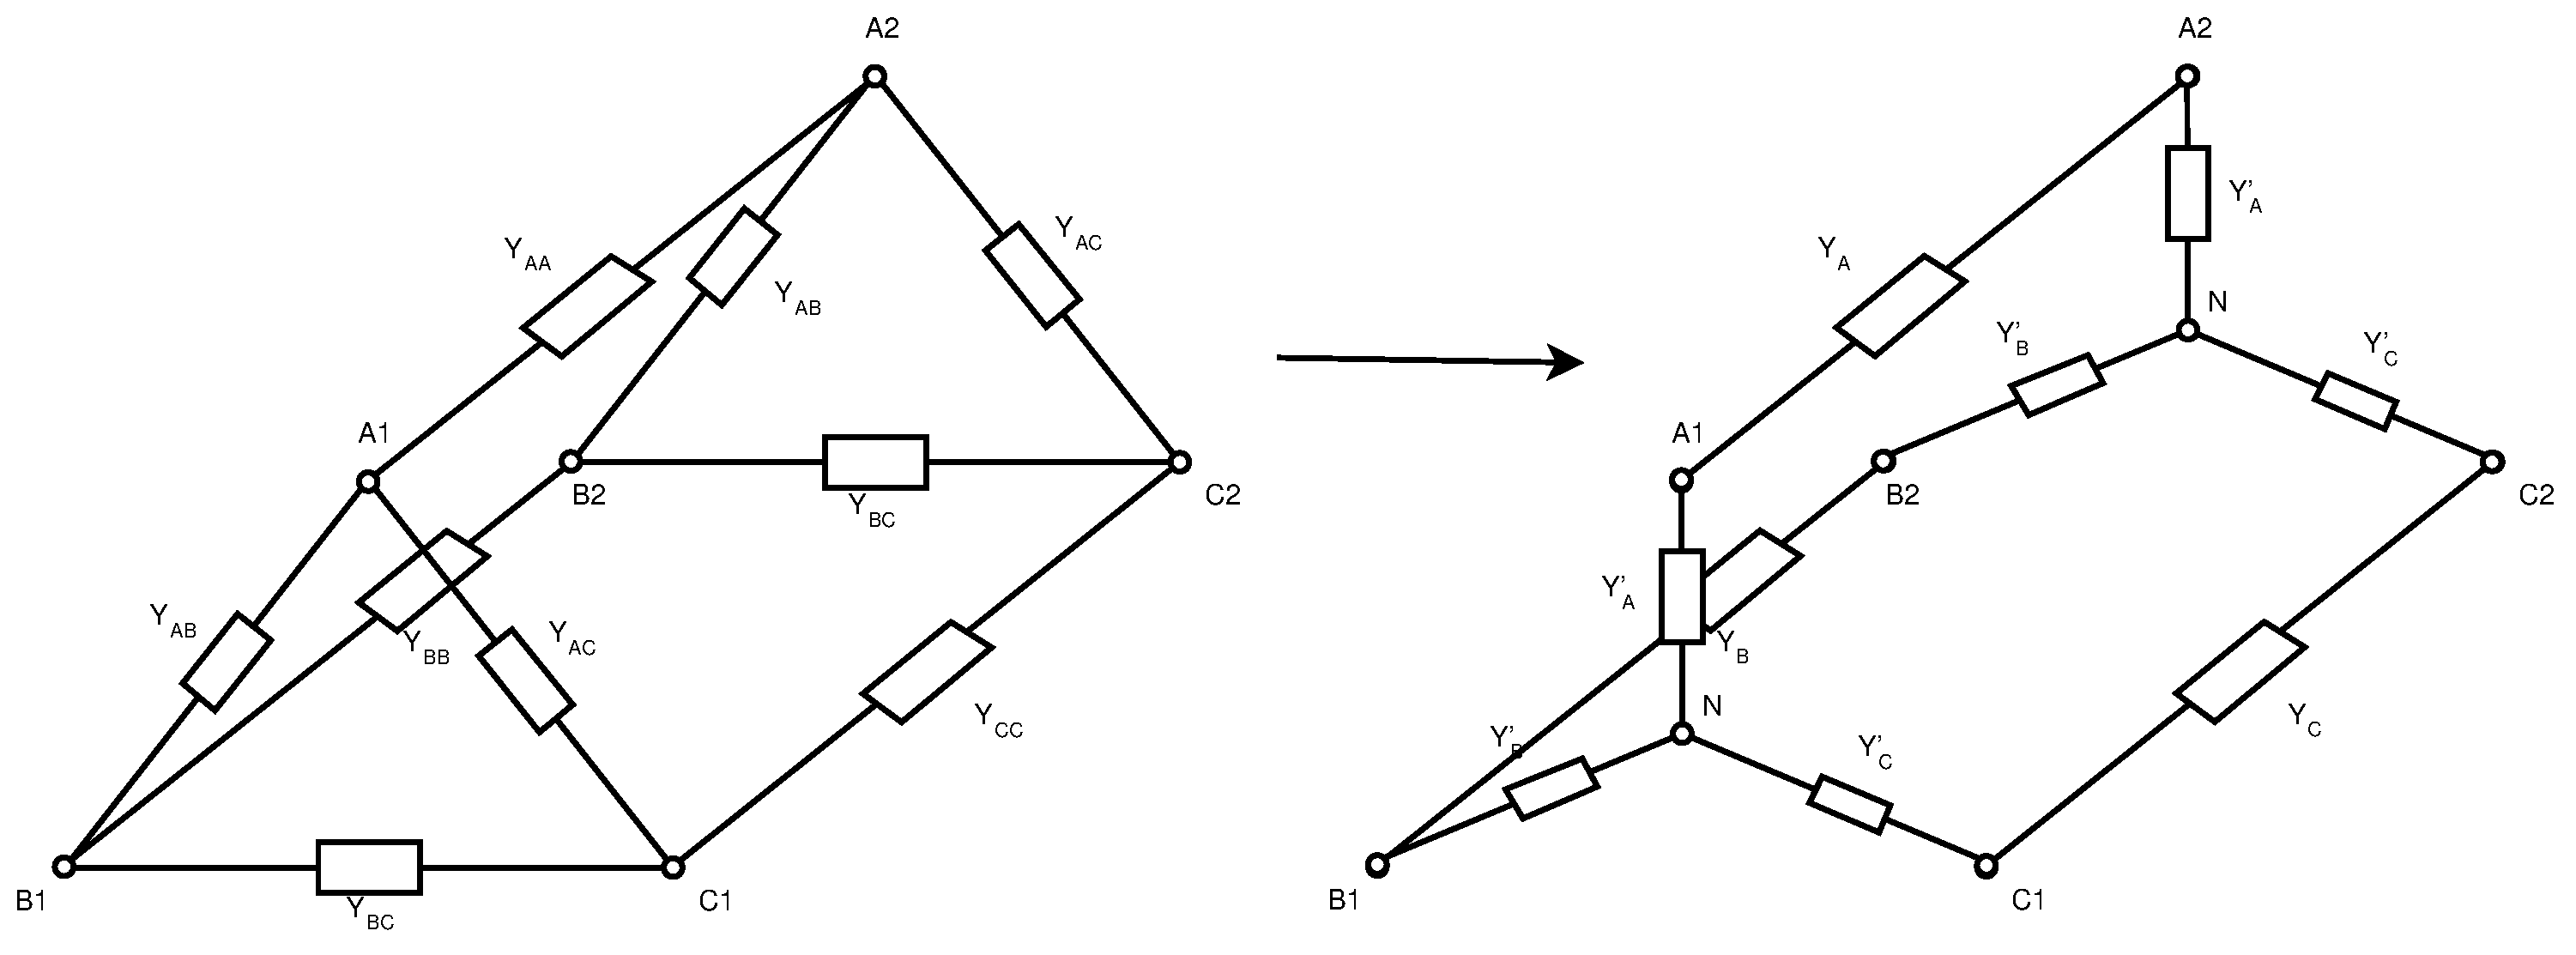
\includegraphics[width=\linewidth]{img/D-Y-Branch.eps}
	\caption{Conversion from the Delta branch model to the Y branch model.}
	\label{fig:DYBranch}
\end{figure}

The three-phase series admittance matrix can be immediately split into three single-phase systems each of them represented by one of the admittances of the diagonal of the three-phase matrix. However by doing this we would be neglecting the phase coupling that is present in the 3x3 matrix.
$$
Y_{series, \Delta} = \left[ \begin{array}{ccc}
Y_{AA} & Y_{AB} & Y_{AC} \\
Y_{BA} & Y_{BB} & Y_{BC} \\ 
Y_{CA} & Y_{CB} & Y_{CC}
\end{array} \right] \longrightarrow Y_{AA}, Y_{BB}, Y_{CC}, couplings?
$$

In order to take into account the phase couplings we need to perform the delta to star conversion of the magnitudes.

\begin{equation}
\left[ \begin{array}{c}
Y_A' \\
Y_B' \\
Y_C'
\end{array} \right] = \left[ \begin{array}{ccc}
1 & -1 & 0 \\
0 & 1 & -1 \\
-1 & 0 & 1
\end{array} \right] \times \left[ \begin{array}{c}
Y_{AB} + Y_{AC} \\
Y_{BC} + Y_{BA}\\
Y_{CA} + Y_{CB}
\end{array} \right]
\end{equation}

$Y_A'$, $Y_B'$ and $Y_C'$ are the shunt magnitudes that appear by embedding the phase-phase coupling admittances by performing the delta-star transformation.

Now we can perform the same operation on the shunt admittance matrix:

$$
Y_{shunt, \Delta} = \left[ \begin{array}{ccc}
Y_{sh,AA} & Y_{sh,AB} & Y_{sh,AC} \\
Y_{sh,BA} & Y_{sh,BB} & Y_{sh,BC} \\ 
Y_{sh,CA} & Y_{sh,CB} & Y_{sh,CC}
\end{array} \right] \longrightarrow Y_{sh,AA}, Y_{sh,BB}, Y_{sh,CC}, couplings?
$$


\begin{equation}
\left[ \begin{array}{c}
Y_{sh, A}' \\
Y_{sh, B}' \\
Y_{sh, C}'
\end{array} \right] = \left[ \begin{array}{ccc}
1 & -1 & 0 \\
0 & 1 & -1 \\
-1 & 0 & 1
\end{array} \right] \times \left[ \begin{array}{c}
Y_{sh,AB} + Y_{sh,AC} \\
Y_{sh,BC} + Y_{sh,BA}\\
Y_{sh,CA} + Y_{sh,CB}
\end{array} \right]
\end{equation}

Finally we can formulate the three single-phase systems:

\begin{itemize}
	\item System A
	
	$Y_{series} = Y_{AA} $\newline
	$Y_{shunt} = Y_{sh, AA} + Y_{A}' + Y_{sh, A}'$
	
	\item System B
	
	$Y_{series} = Y_{BB} $\newline
	$Y_{shunt} = Y_{sh, BB} + Y_{B}' + Y_{sh, B}'$
	
	\item System C
	
	$Y_{series} = Y_{CC} $\newline
	$Y_{shunt} = Y_{sh, C} + Y_{C}' + Y_{sh, C}'$
\end{itemize}

In Matrix form:

\begin{equation}
\left[ \begin{array}{c}
Y_{series,decoupled,A} \\
Y_{series,decoupled,B} \\
Y_{series,decoupled,C}
\end{array} \right] = \left[ \begin{array}{c}
Y_{AA} \\
Y_{BB} \\
Y_{CC}
\end{array} \right]
\end{equation}

\begin{equation}
\left[ \begin{array}{c}
Y_{sh, decoupled, A} \\
Y_{sh, decoupled, B} \\
Y_{sh, decoupled, C}
\end{array} \right] = \left[ \begin{array}{c}
Y_{sh,A} \\
Y_{sh,B} \\
Y_{sh,C}
\end{array} \right] + \left[ \begin{array}{ccc}
1 & -1 & 0 \\
0 & 1 & -1 \\
-1 & 0 & 1
\end{array} \right] \times \left[ \begin{array}{c}
Y_{AB} + Y_{AC} + Y_{sh,AB} + Y_{sh,AC} \\
Y_{BC} + Y_{BA} + Y_{sh,BC} + Y_{sh,BA}\\
Y_{CA} + Y_{CB} + Y_{sh,CA} + Y_{sh,CB}
\end{array} \right]
\end{equation}



%-------------------------------------------------------------------------------
%	CHAPTER The bus and it's connected elements
%-------------------------------------------------------------------------------
\chapter{The bus and it's connected elements}

The bus model is based upon the traditionally called \textit{ZIP} bus model to indicate that the same model includes an impedance ($Z$), a current ($I$) and a power ($P$) value. To be consistent with our nomenclature, here we are going to refer to it as the $YISV$ model since at the node there is voltage($V$), and a power ($S$), an admittance ($Y$) and a current ($I$) potentially connected.


\begin{marginfigure}
	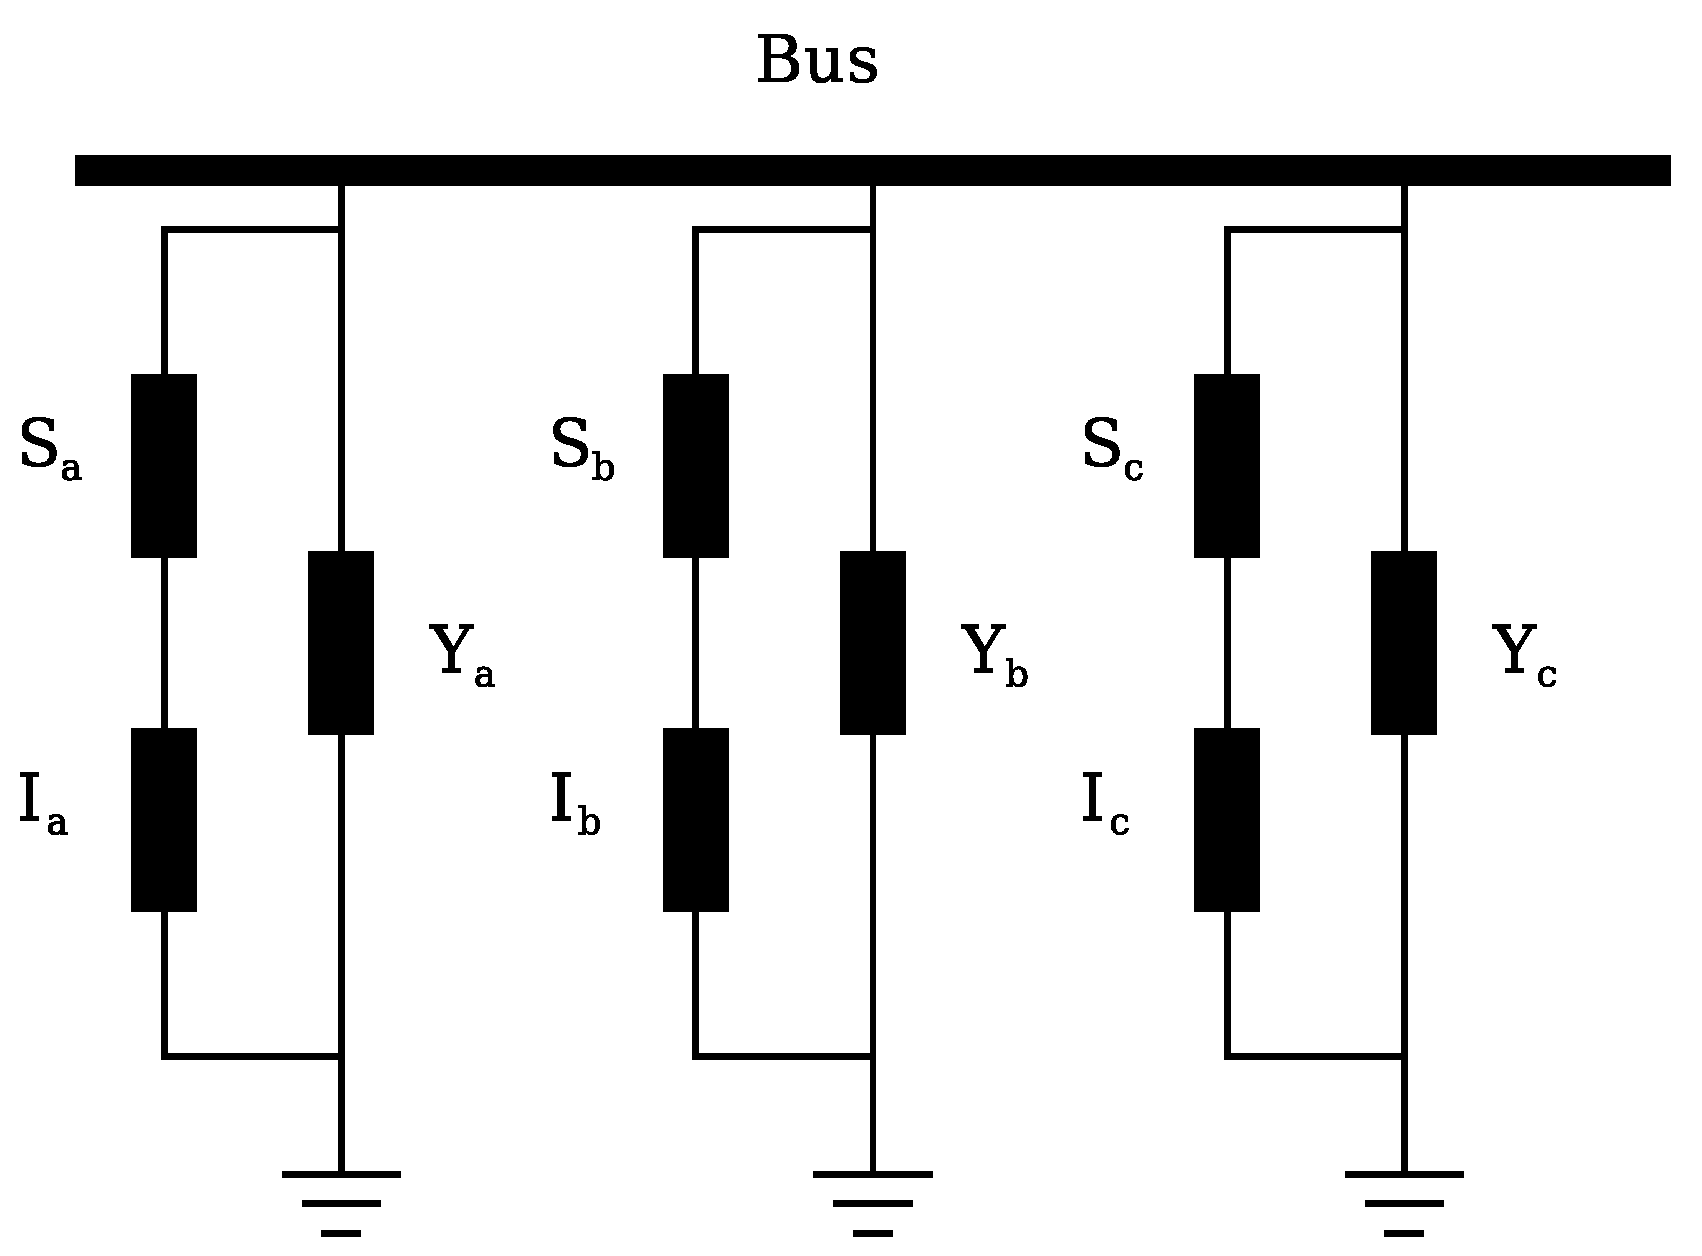
\includegraphics[width=0.99\linewidth]{img/NodeElements.eps}
	\caption{$YISV$ Bus model.}
	\label{bus_model}
\end{marginfigure}

The admittance, power and current values at the bus are derived from the elements connected to it (loads, generators, capacitor banks, etc.)


\section{The substation}

In reality a substation is a collection of real bus bars (metal bars usually made of copper or aluminium) switchgear and shunt devices. The use of a substation is to change the connectivity topology of the grid.

For calculation, the substation connectivity is solved first, originating one or more calculation buses. Therefore, the substations are irrelevant at calculation level, but they are very relevant in the definition of the grid topology prior to the calculation.

\begin{figure}
	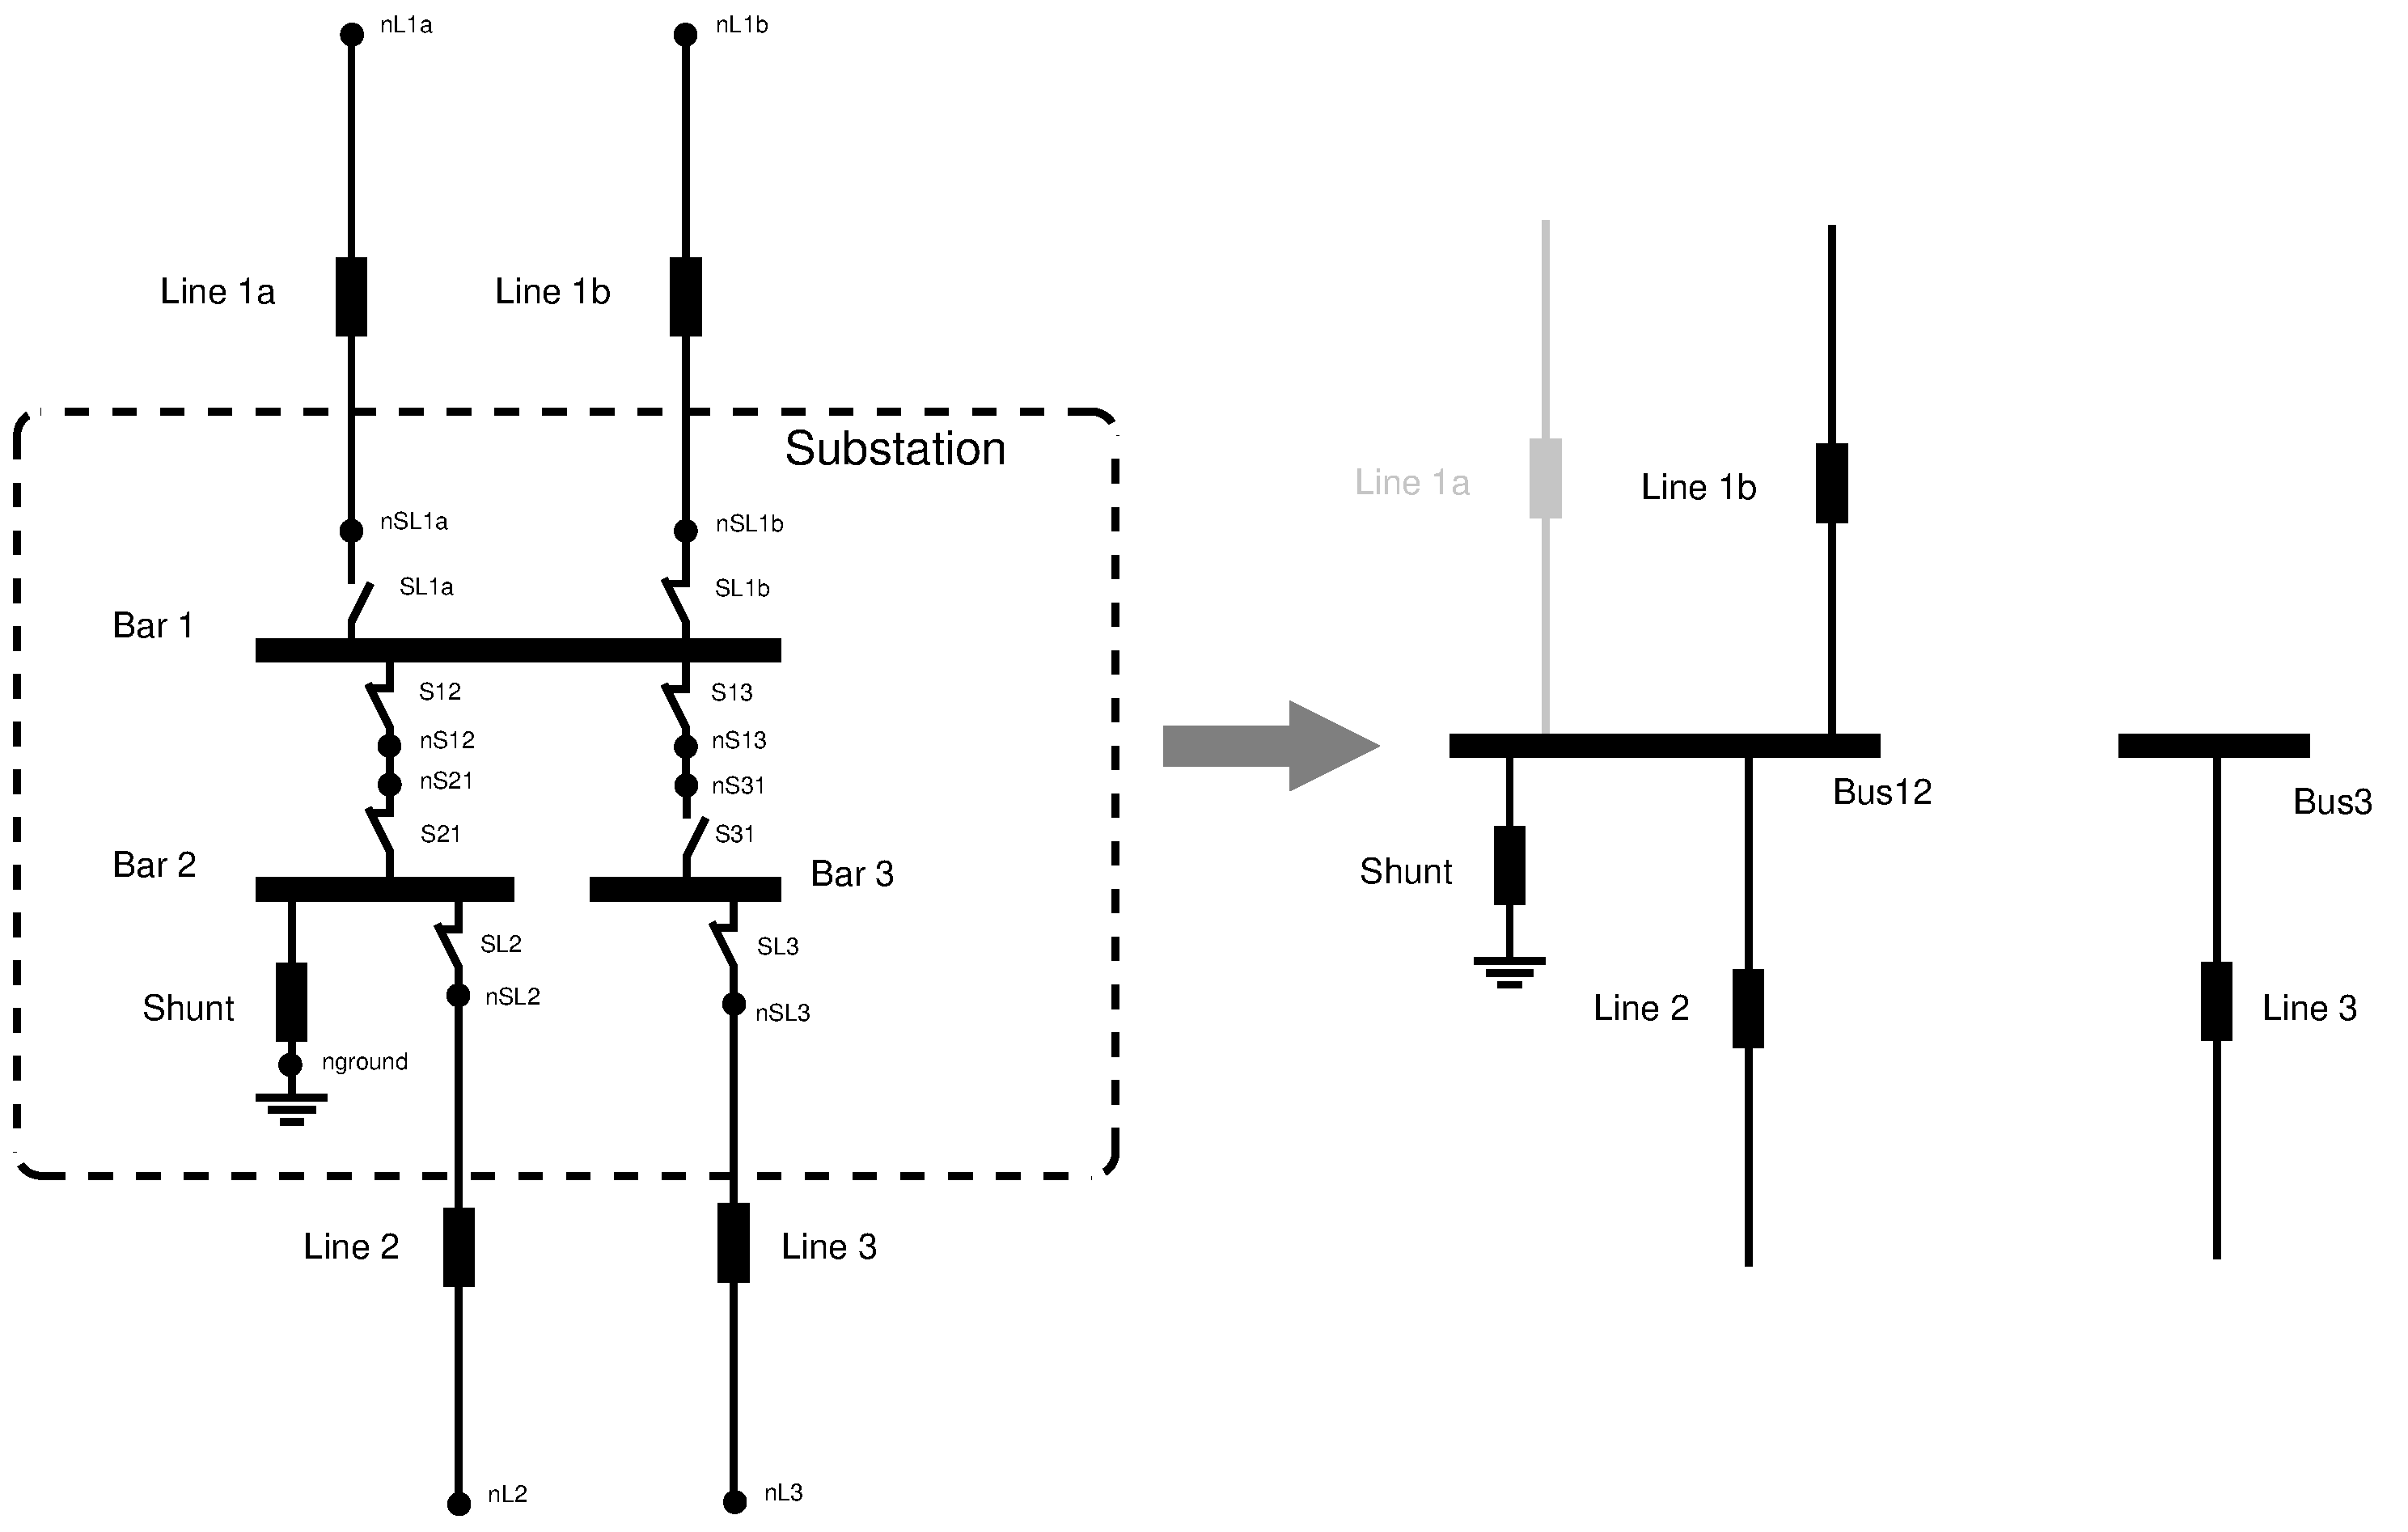
\includegraphics[width=0.99\linewidth]{img/Substation.eps}
	\caption{Substation example. The substation becomes a calculation bus.}
	\label{substation_model}
\end{figure}

In the example depicted in the figure \ref{substation_model} it is shown how a node system is reduced from three real buses to two calculation buses by eliminating the non connected elements and associating the connected ones. The buses1, 2 are connected because the switches between them are closed, hence the three buses become one. the bus 3 is isolated from the others, but still connected to a line. The lines 1b, 2 and 3 are also connected through closed switches, hence those remain connected to their respective buses. However the line 1a is connected through an open switch, therefore is left out for calculation purposes.

In order to calculate this reduction, we need to introduce extra nodes in the substation model. These are topological nodes that will help us to perform the connectivity calculation. Then we represent the substation as a node-branch graph:

\begin{center}
\begin{figure}
	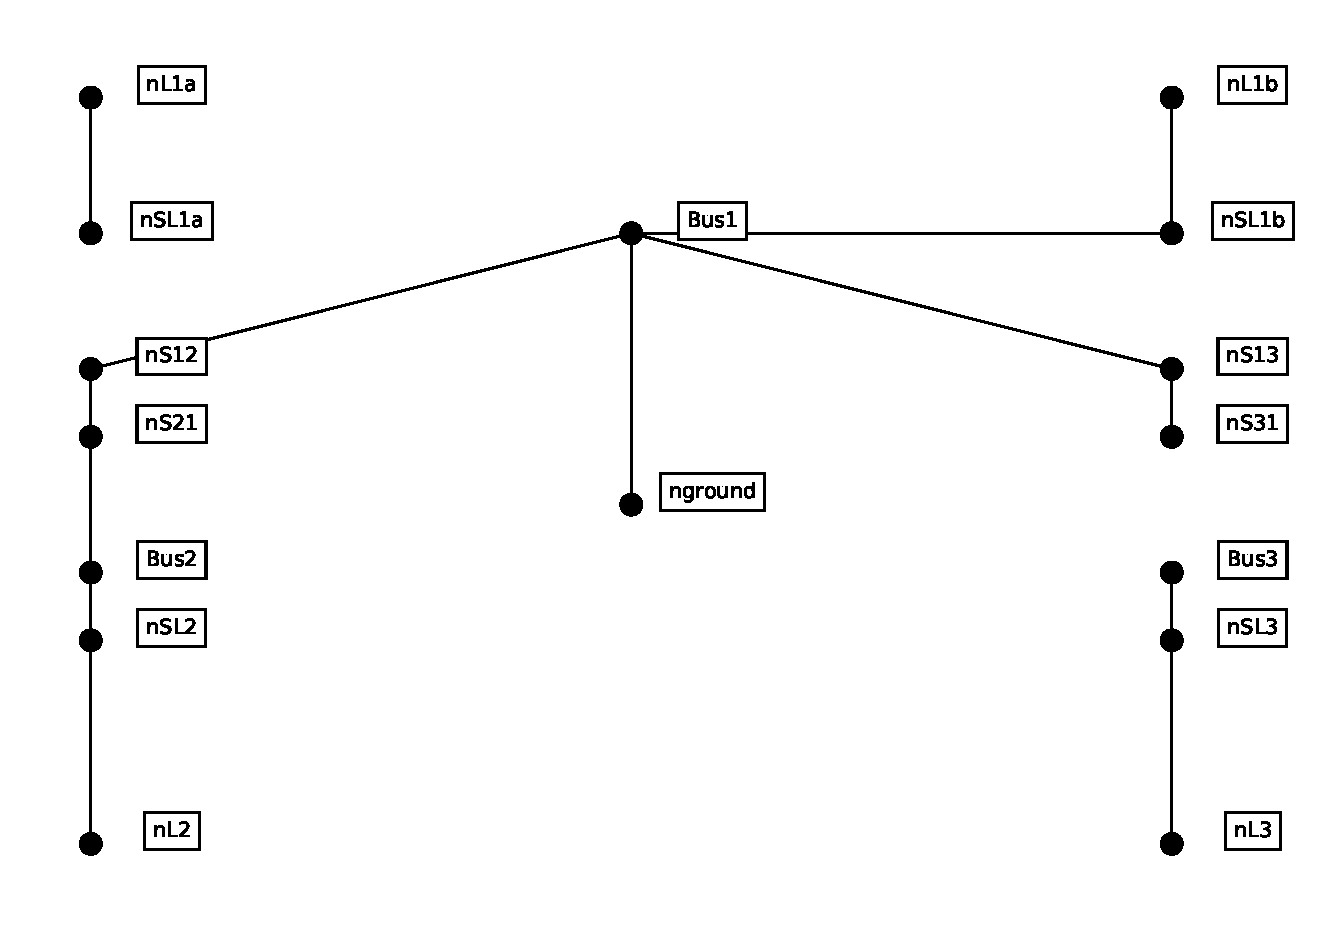
\includegraphics[width=0.6\linewidth]{img/Substation_graph.eps}
	\caption{Substation example graph.}
	\label{substation_graph}
\end{figure}
\end{center}


Observe the islands formed:

\begin{itemize}
	\item Island 1: \textbf{Bus1}, \textbf{Bus2}, nL1b, nL2, nS12, nS13, nS21, nS31, nSL1b, nSL2, nground.
	\item Island 2: \textbf{Bus3}, nL3, nSL3.
	\item Island 3: nL1a, nSL1a.
\end{itemize}

Removing the topological nodes, only two islands remain:

\begin{itemize}
	\item Island 1: \textbf{Bus1, Bus2}.  -> these two form a joint calculation node.
	\item Island 2: \textbf{Bus3}.
\end{itemize}

Now we only need to check which non topological branches are in every island and associate them to the formed calculation node.

\section{Load}

The modelling of a load is done as a composition of fixed impedance, fixed current and fixed power. This is known to match best the real behaviour of loads in electrical grids (Although in transmission they tend to be more fixed power-dominated). This is known as the ZIP model of a load. Here we are going to refer to it as ZIS, given that we actually specify the complex power ($S$) and not the real power ($P$).

\begin{marginfigure}
	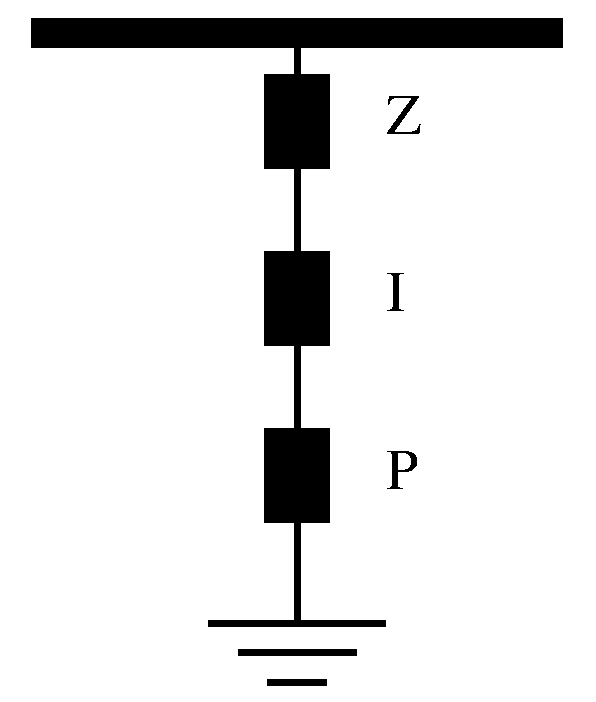
\includegraphics[width=0.49\linewidth]{img/ZIP_model.eps}
	\caption{$ZIP$ Bus model.}
	\label{zip_bus_model}
\end{marginfigure}

The main calculation parameters of a load are:\\
\begin{tabular}{|l|p{3cm}|p{4cm}|}
	\hline 
	Parameter & Description & Unit \\ 
	\hline 
	Z & Impedance (complex number) & MW, MVAr at the bus nominal voltage \\ 
	\hline 
	I & Current (complex number) & MW, MVAr at the bus nominal voltage \\ 
	\hline 
	S & Power (complex number) & MW, MVAr \\ 
	\hline
\end{tabular} 

\vspace{0.5cm}

The impedance $Z$ is converter to admittance with $Y=1/Z$.

When the systems matrix are forming, the admittance ($Y$) is added to the diagonal of the admittance matrix ($Ybus$ or simply $Y$), the power ($S$) os added to the power injections vector ($Sbus$ or simply $S$) and the current is added to the current injections vector ($Ibus$ or simply $I$).

Remember that the system power equilibrium equation is:

$$
S_{bus} = V_{bus} \cdot (I_{bus} + Y_{bus} \times V_{bus})^*
$$


\section{Voltage controlled generator}

A voltage controlled generator is a generator that sets the voltage of the bus where it is connected.

The main parameters of a voltage controlled generator are:\\
\begin{tabular}{|l|p{5cm}|p{2cm}|}
	\hline 
	Parameter & Description & Unit \\ 
	\hline 
	$V_{set}$ & Set voltage (number) & p.u. \\ 
	\hline 
	$P$ & Power (number) & MW \\ 
	\hline
	$Q_{min}$ & Reactive power lower limit (number) & MVAr \\ 
	\hline
	$Q_{max}$ & Reactive power upper limit (number) & MVAr \\ 
	\hline
\end{tabular} 

\vspace{0.5cm}

%When forming the 

\section{Battery}

A battery shall be modelled as a voltage controlled generator.

The main parameters of a voltage controlled generator are:\\
\begin{tabular}{|l|p{5cm}|p{2cm}|}
	\hline 
	Parameter & Description & Unit \\ 
	\hline 
	$V_{set}$ & Set voltage (number) & p.u. \\ 
	\hline 
	$P$ & Power (number) & MW \\ 
	\hline
	$Q_{min}$ & Reactive power lower limit (number) & MVAr \\ 
	\hline
	$Q_{max}$ & Reactive power upper limit (number) & MVAr \\ 
	\hline
	$E_{max}$ & Energy storage capacity (number) & MWh \\ 
	\hline
\end{tabular} 

\vspace{0.5cm}


\section{Capacitor banks}




%-------------------------------------------------------------------------------
%	CHAPTER Topology analysis and consolidation
%-------------------------------------------------------------------------------
\chapter{Topology analysis and consolidation}


\section{Islands detection}


\section{Calculation of the bus connected phases}

\newpage
\section{Calculation of the admittance matrices}  \label{Y_calculation}

For the computations ahead we will need to have a number of admittance-based matrices. Remember that these matrices are only valid for island circuits, this is a multi-island circuit will have a set of these matrices per island. Otherwise the matrices would be singular.

\begin{itemize}
	
	\item $n$: Number of buses.
	
	\item $m$: Number of branches.
	
	\item $Y_{bus}$ or simply $Y$: Complete admittance matrix.
	
	It is a sparse matrix of size $n \times n$
	
	\item $Y_{series}$: Admittance matrix of the series elements. It contains no value coming from shunt elements or the shunt parts of the branch model.
	
	It is a sparse matrix of size $n \times n$
	
	\item $Y_{shunt}$: Admittance vector of the shunt elements and the shunt parts of the branch model. 
	
	It is a vector of size $n$
	
	\item $Y_f$: Admittance matrix of the branches with their \textit{from} bus.
	
	It is a sparse matrix of size $m \times n$
	
	\item $Y_t$: Admittance matrix of the branches with their \textit{to} bus.
	
	It is a sparse matrix of size $m \times n$\newline
\end{itemize}

Where $n$ is the number of buses and $m$ is the number of branches.

The relation between the admittance matrix and the series and shunt admittance matrices is the following:
\begin{equation}
Y_{bus} = Y_{series} + Y_{shunt}
\end{equation}

The algorithmic logic to build the matrices in pseudo code is the following:

\begin{verbatim}
n = number of buses in the circuit
m = number of branches in the circuit

// declare the matrices
Y = complex_sparse(n, n)
Yf = complex_sparse(m, n)
Yt = complex_sparse(m, n)
yshunt = complex_vector(n)
yseries = complex_sparse(n, n)

// set the buses admittances
for i=0 to n:

    // get all the bus-connected power, current andmittance and voltage
    y, curr, s, v = buses[i].get_YISV()

    Yshunt[i] = y
end

//set the branches admittances
for i=0 to m:
    // get the bus indices matching the busses of this branch
    f = get_bus_index(branches[i].bus_from)
    t = get_bus_index(branches[i].bus_to)
    
    // compose the basic elements (only for pisitive sequence)
    z_series = complex(branches[i].R, branches[i].X)
    y_shunt = complex(branches[i].G, branches[i].B)
    tap = branches[i].tap_module * exp(-1j * branches[i].angle)
    Ysh = y_shunt / 2
    Ys = 1 / z_series

    // compose the matrix sub elements
    Ytt = Ys + Ysh
    Yff = Ytt / (tap * conj(tap))
    Yft = - Ys / conj(tap)
    Ytf = - Ys / tap    
    Yff_sh = Ysh
    Ytt_sh = Yff_sh / (tap * conj(tap))
    
    // Full admittance matrix
    Ybus[f, f] += Yff
    Ybus[f, t] += Yft
    Ybus[t, f] += Ytf
    Ybus[t, t] += Ytt
    
    // Y-from and Y-to for the lines power flow computation
    Yf[i, f] += Yff
    Yf[i, t] += Yft
    Yt[i, f] += Ytf
    Yt[i, t] += Ytt
    
    // Y shunt
    Yshunt[f] += Yff_sh
    Yshunt[t] += Ytt_sh
    
    // Y series
    Yseries[f, f] += Ys / (tap * conj(tap))
    Yseries[f, t] += Yft
    Yseries[t, f] += Ytf
    Yseries[t, t] += Ys
end

\end{verbatim}


\section{Calculation of the voltage, power and current vectors}


%-------------------------------------------------------------------------------
%    CHAPTER Power flow
%-------------------------------------------------------------------------------
\chapter{Power flow} \label{ch:power_flow}

The power flow problem consists in finding the node voltages that correspond to the injected current and power values. The fundamental equation to be solved is:

\begin{equation}
S = V \times (Y \times V - I)^*
\label{eq:power_flow}
\end{equation}

\marginnote{Note that the equation \ref{eq:power_flow} is non-linear when solving for the voltage ($V$). However if there are no power injections and only current injections, the equation becomes linear. Because of the non-linearity, we will be using iterative methods to solve this equation.}

Where:

\begin{itemize}
\item $S$: Vector of power injections.
\item $I$: Vector of current injections.
\item $V$: Vector of voltages.
\item $Y$: Admittance matrix.
\end{itemize}


\section{Types of buses}

At each node, we can consider the following magnitudes to exist:
\begin{itemize}
	\item $|V|$: Voltage module.
	\item $\delta$: Voltage angle.
	\item $P$: Active power injection/consumption.
	\item $Q$: Reactive power injection/consumption.
\end{itemize}

In some nodes we know the active power injection (generation nodes), in some nodes we just know the consumption power (load nodes), and in some nodes we artificially define the voltage (slack nodes). The power flow problem is formulated such that in every node two variables are set and the other two are computed. Thus we can define the node types as:

\begin{table}[h!]
	\begin{center}
		\begin{tabular}{ccccc}
			\toprule
			
			Bus type & $|V|$ &  $\delta$ & $P$ & $Q$\\
			
			\midrule
			
			$PQ$ & Calc. &  Calc. & Set & Set\\
			$PV$ & Set &  Calc. & Set & Calc.\\
			$VD$ (slack) & Set &  Set & Calc. & Calc.\\
			
			
			\bottomrule
		\end{tabular}
	\end{center}
	\caption{Bus types.}
	\label{bus__types}
\end{table}

There must be at least one $VD$ or slack node in order to be able to compute the power flow problem. 



\section{Z-Matrix}

The Z-Matrix method is a simple iterative method that provides good results, especially in distribution grids where the voltage variations are not large.

The Z-Matrix method requires the Kron reduction of the slack nodes of the circuit. This reduction is explained below:

\begin{figure}[h!]
  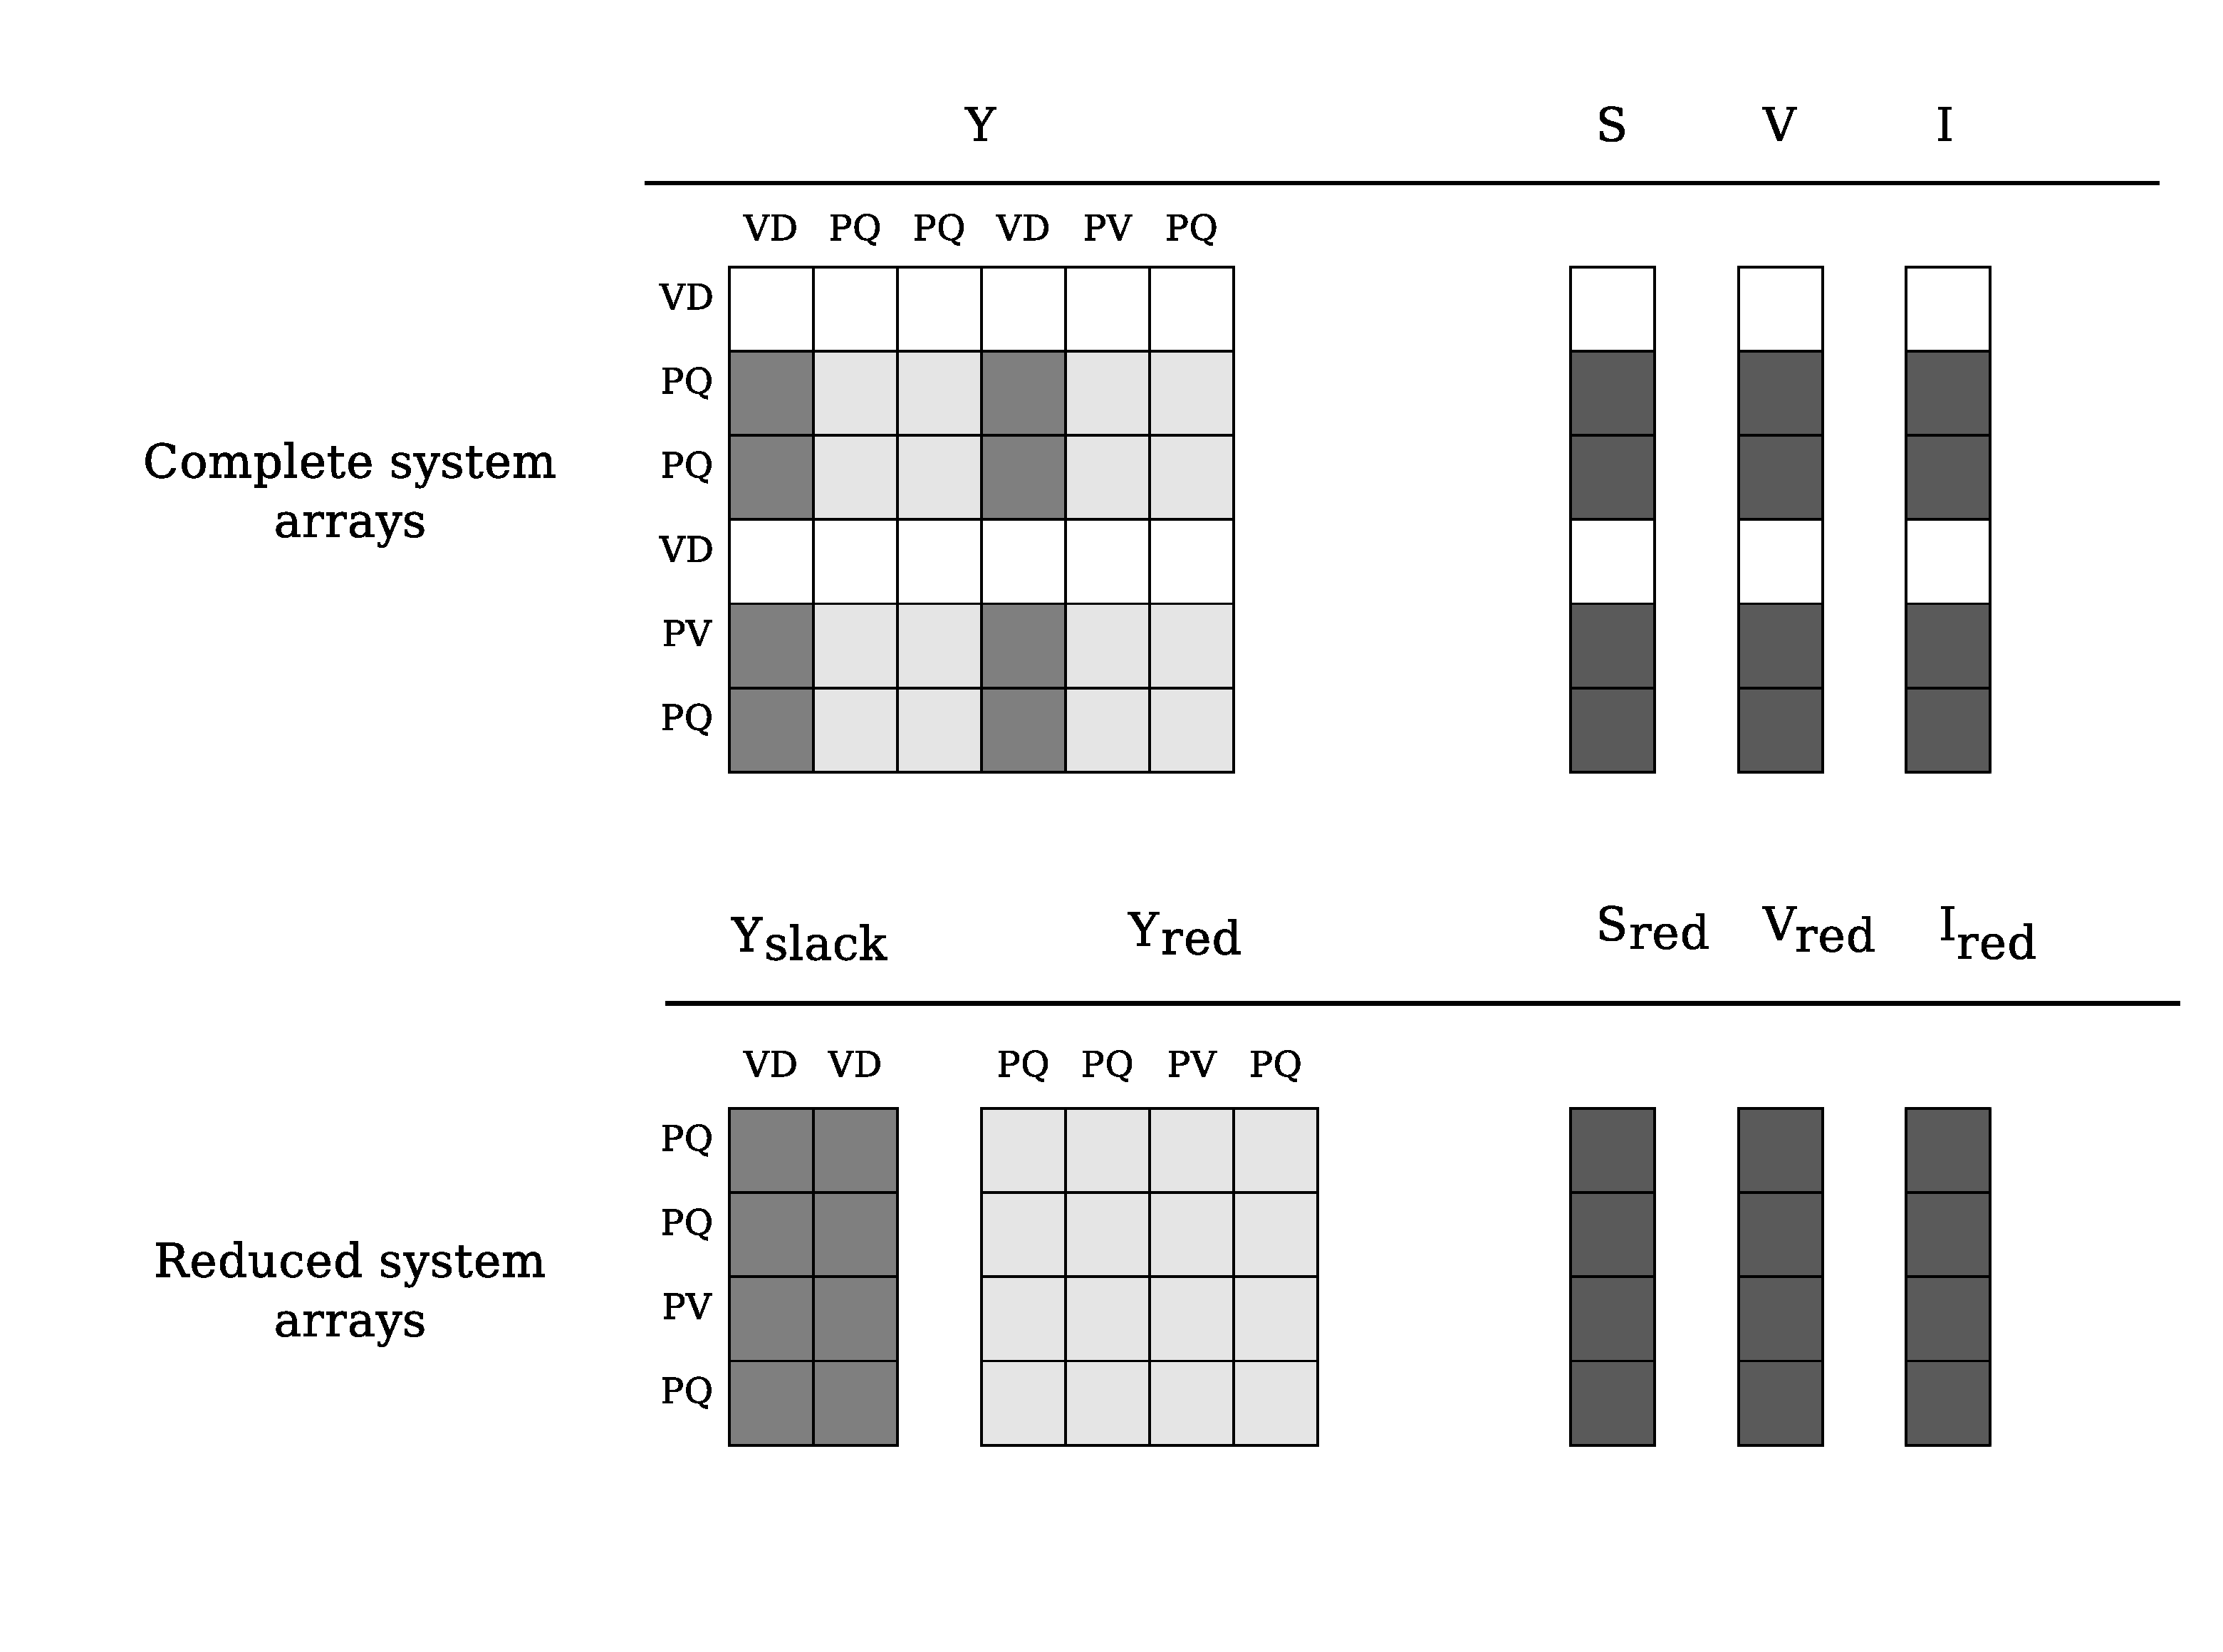
\includegraphics[width=\linewidth]{img/Matrix_reduction.eps}
  \caption{Circuit's admittance matrix and vectors reduction. Representation for a six node circuit with two slack nodes.}
  \label{fig:reduction}
\end{figure}

\begin{equation}
Y_{red} = Y[pqpv, pqpv]
\end{equation}

\begin{equation}
Y_{slack} = Y[pqpv, vd]
\end{equation}

\begin{equation}
V_{red} = V[pqpv]
\end{equation}

\begin{equation}
V_{slack} = V[vd]
\end{equation}

\begin{equation}
S_{red} = S[pqpv]
\end{equation}

\begin{equation}
I_{red} = I[pqpv]
\end{equation}

Once we have all the reduced magnitudes, it means that we have removed the slack (VD) nodes from the circuit, but we must keep their influence in the rest of the nodes in the form of current injections.

First we copy $V_{red}$ into another variable $V_{prev}$.

\begin{equation}
V_{prev} = V_{red}
\end{equation}

The current injections appearing by the removal of the slack nodes are:
\begin{equation}
I_{slack} = Y_{slack} \times V_{slack}
\end{equation}

The voltages that arise from the slack current injections are:
\begin{equation}
C_k = Y_{red} \times I_{slack}
\end{equation}

The total injected currents including the power injections are:
\begin{equation}
I_k = \frac{S_{red}}{V_{prev}} + I_{red}
\label{eq:zm_ik}
\end{equation}

The next step is to compute the nodes voltage due to all the power and current injections:

\begin{equation}
V_k = Y_{red}^{-1} \times I_k - C_k
\end{equation}

Now the error is the infinite norm of the voltage difference.

\begin{equation}
error = ||V_{prev} - V_k ||_{\infty} = max(abs(V_{prev} - V_k ))
\end{equation}

The infinite norm of the voltage difference between the previous iteration and the current iteration is a poor convergence criteria, but it is usually the only working criteria in practice for this method.

Now we need to correct the voltage for the PV nodes so that they control the voltage module.

\begin{equation}
V_{k}[pv_{red}] = V_k \cdot \frac{|V^{esp}[pv_{red}]|}{|V_{k}[pv_{red}]|}
\label{eq:zm_pv_correction}
\end{equation}

\marginnote{Note that $pv_{red}$ is the vector of pv node indices in the reduced scheme. It is not equal to the $pv$ indices vector.}

Next, we copy the voltage solution to the previous voltage solution vector:

\begin{equation}
V_{prev} = V_k
\label{eq:zm_copy_sol}
\end{equation}

Repeat equations \ref{eq:zm_ik} to \ref{eq:zm_copy_sol} until the error is less or equal to a given tolerance not too strict like $1\times10^{-3}$.

Finally, since we have found the voltages for the PQ and PV nodes only, we should return a voltage vector with the voltages for all the nodes. Because of this, we copy the voltage solution for the reduced system into a copy of the original voltage vector.

\begin{equation}
V[pqpv] = V_k
\end{equation}


\section{Jacobian based power flow}

The derivative based methods are more accurate than the derivative free methods. They are usually more robust at the cost of being more computationally expensive. In this section we'll start by introducing the Jacobian matrix. It is the derivative of the power flow equation  [\ref{eq:power_flow}] with respect to a set of voltage values. The section continues by introducing the methods that use this matrix to solve the power flow problem.

\begin{center}
\begin{figure}[h!]
  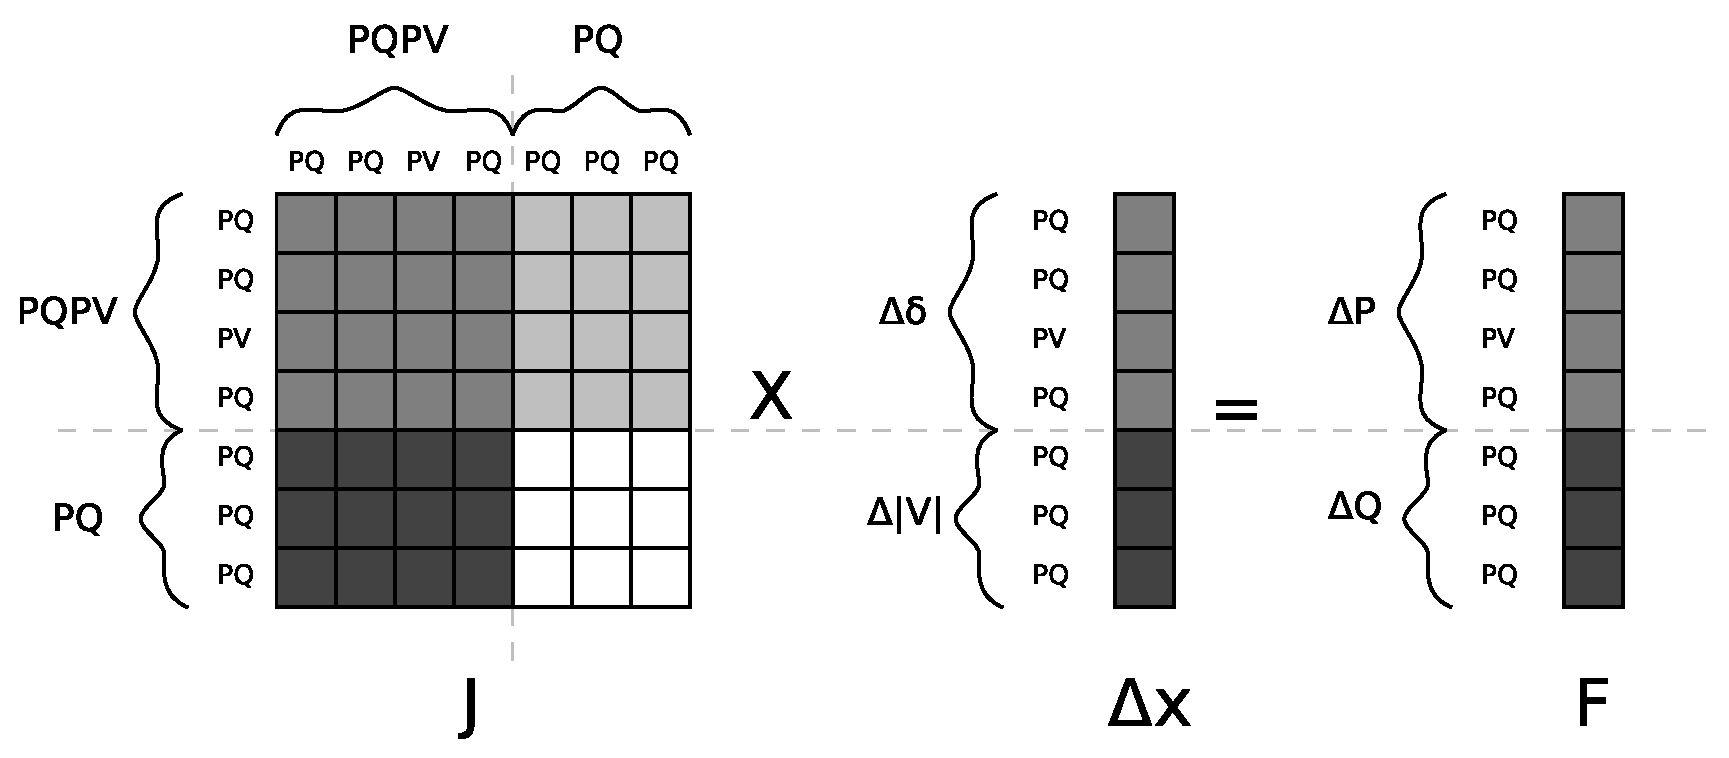
\includegraphics[width=0.9\linewidth]{img/JacobianBased.eps}
  \caption{Jacobian based linear system to compute the voltage increments.}
  \label{fig:jacobian_based}
\end{figure}
\end{center}

The Jacobian linear system ($J \times \Delta x = F$), allows the computation of the voltage increment ($\Delta x$) to apply to the voltage solution ($V$) in order to achieve a voltage that solves the power flow equation \ref{eq:power_flow}. This process is iterative and recursive, hence to have a initial voltage solution in the vicinity of the final solution is crucial. Otherwise the method will converge to a non physical solution. A common good-enough voltage initial solution is to set all the voltages according to the slack voltage value.


\subsection{Building the Jacobian matrix} \label{Jacobian_chapter}

The Jacobian matrix ($J$) is the derivative of the fundamental power flow equation \ref{eq:power_flow}, with respect to the voltage magnitudes to be solved $|V|$ and $\delta$. It is one of the most expensive parts of the derivative based power flow methods.

In most literature, the reader will find the Jacobian presented with non matrix formulas which are hard to understand in their relation to the Jacobian matrix formation. Ray D. Zimmerman came up with a fantastic way of building the Jacobian matrix \cite{zimmerman2010ac} by using lineal algebra operations over the complex matrices and vectors that represent the circuit. The formulation presents a huge advantage: No use of cosine and sine operations for the derivatives computation. The calculation of trigonometric functions is a recursive operation and should be avoided whenever possible in high performance computing. The formulation is presented as follows.

First we compute the total current injection. It is a sparse diagonal matrix, so do not use a dense matrix format.
\begin{equation}
I_{diag} = diag(Y \times V - I)
\end{equation}

Then we convert the buses voltage solution $V$ into a square diagonal matrix. Use a sparse format for this.
\begin{equation}
V_{diag} = diag(V)
\end{equation}

Compute the buses voltage normalized solution $V$ into a square diagonal matrix. This is acomplished by dividing each complex voltage by its absolute value. Use a sparse format for this.
\begin{equation}
E_{diag} = diag(V / |V|)
\end{equation}

Now, Compute the derivative of the power injections $S$ with respect to the voltage module $|V|$:
\begin{equation}
\frac{\partial S}{\partial |V|} = V_{diag} \times (Y \times E_{diag})^* + I_{diag}^* \times  E_{diag}
\end{equation}
    
Compute the derivative of the power injections $S$ with respect to the voltage angle $\delta$:
\begin{equation}
\frac{\partial S}{\partial \delta} = 1j \cdot V_{diag} \times (I_{diag} - Y \times V_{diag})^*
\end{equation}

Finally, assemble the Jacobian matrix $J$. The Jacobian matrix is sparse and only contains real values. If the circuit contains $npq$ buses of type $PQ$ and $npv$ buses of type $PV$, the Jacobian matrix is a square matrix with $2 npq + npv$ rows and the same number of columns. See the figure \ref{fig:jacobian_based}.

\begin{equation}
J=
\left[
\begin{array}{cc}
Re\left(\frac{\partial S}{\partial \delta}[pqpv, pqpv]\right) &
Re\left(\frac{\partial S}{\partial |V|}[pqpv, pq]\right) \\
Im\left(\frac{\partial S}{\partial \delta}[pq, pqpv]\right) &
Im\left(\frac{\partial S}{\partial |V|}[pq, pq]\right)
\end{array}
\right]
\end{equation}

Observe that the Jacobian matrix is composed of four subsets of the previously computed derivatives $\frac{\partial S}{\partial \delta}$ and $\frac{\partial S}{\partial |V|}$, where combinations of the $PQ$ and $PV$ node indices are selected.

$pqpv$ is a vector that contains the indices of the $PQ$ and $PV$ type indices in sequential order.

$pq$ is a vector that contains the indices of the $PQ$  type indices in sequential order.

\newpage
\subsection{Newton-Raphson}

Newton-Raphson is a recursive, iterative numerical method that minimizes the value of a function. In our case the value to minimize is the power mismatch:

\begin{equation}
\Delta S = S_{specified} - S_{calc} 
\end{equation}

Where:
\begin{equation}
s_{calc} = V \times (Y \times V - I_{bus})^*
\label{eq:nr_Scalc}
\end{equation}

The minimization of $\Delta S$ occurs via se recursive solution of the following linear system:

\begin{equation}
J \times \Delta x = F
\end{equation}

Since the mismatch ($\Delta S$) is a vector of complex values, we transform it into a vector ($F$) with the real part of $\Delta S$ for the PQ and PV bus indices and the imaginary part of $\Delta S$ for the PQ bus indices of the vector. Observe that the length of the vector is $2npq+npv$, matching the Jacobian dimensions.



\begin{equation}
F =  \left[
\begin{array}{c}
\Delta P \\
\Delta Q  
\end{array}
\right]
\label{eq:nr_mismatch}
\end{equation}

\begin{equation}
\Delta Q = Im(\Delta S[pq]) 
\label{eq:nr_q_inc}
\end{equation}

\begin{equation}
\Delta P = Re(\Delta S[pqpv])
\label{eq:nr_p_inc}
\end{equation}

Then we define the error to minimize as the infinite norm of $F$. The infinite norm is the same as the maximum absolute value. If the error is less than the specified tolerance, we stop the iterations otherwise, continue until a certain number of iterations considered as the maximum (for example 20).

\begin{equation}
error = ||F||_{\infty} = max(abs(F))
\label{eq:nr_error}
\end{equation}

If the error is higher than the tolerance, we need to solve the voltages increment ($\Delta x$), for which we must compute the Jacobian first. Some simplifications of the method only compute the Jacobian one time, but for better accuracy, the Jacobian needs to be calculated on every iteration.

\marginnote{Do not invert $J$, instead use a linear system solver, to solve the linear system $J \times \Delta x  = F$.}

\begin{equation}
\Delta x = J^{-1} \times F
\label{eq:nr_solve}
\end{equation}

Notice that $\Delta x$ is a vector with the voltage angles ($\delta$) for the PQ and PV nodes followed by the voltage modules ($|V|$) for the PQ nodes. This matches the way we built the Jacobian ($J$) and the mismatch ($F$). Now we must assign those polar voltage angle and module increments to the rectangular voltage vector that we use to compute the Jacobian and the mismatch.

To accomplish this, we declare two polar voltage increment vectors $\Delta |V|$ and $\Delta \delta$, initialize them to zero, and we fill the corresponding values with the following:

\marginnote{Here we use the auxiliary vectors $pqpv$ and $pq$ which contain the indices of the pq and pv type buses, and the pq type buses respectively. $npqpv$ and $npq$ are the sizes of those two vectors.}
\begin{equation}
\Delta \delta[pqpv[i]] = \Delta x[i]  \quad \forall i \in {0..npqpv}
\label{eq:nr_dd1}
\end{equation}

\begin{equation}
\Delta  |V|[pq[i]] = \Delta x[i+npqpv]  \quad \forall i \in {0..npq}
\end{equation}

Then we need to add those values to the voltage module and angle vectors $|V|$ and $\delta$:

\marginnote{Here we introduce the notion of the $k_{th}$ iteration wich represents the current iteration and the $k_{th}+1$ represents the next iteration.}

\begin{equation}
|V|^{(k+1} = |V|^{(k} + \Delta |V|^{(k}
\end{equation}

\begin{equation}
\delta^{(k+1} = \delta^{(k} + \Delta \delta^{(k}
\end{equation}

At last, we convert the polar vectors  $|V|$ and $\delta$ into a single complex voltage vector $V$.

\begin{equation}
V^{(k+1} = |V|^{(k+1} \cdot \left( cos(\delta^{(k+1}) + 1j \cdot sin(\delta^{(k+1})\right)
\label{eq:nr_voltage_conversion}
\end{equation}

The method consists in repeating formulas \ref{eq:nr_Scalc} to \ref{eq:nr_voltage_conversion} until the error is less or equal to the tolerance or a number of iterations is reached.

The algorithm is then:

\begin{enumerate}

\item Start.

\item Compute the mismatch function ($F$) using the initial voltage solution ($V$). Equation \ref{eq:nr_mismatch}.

\item Compute the error. Equation \ref{eq:nr_error}.

\item While $error > tolerance$ or $iterations < max\_iterations$:

	\begin{enumerate}
	\item Compute the Jacobian
	
	\item Solve the linear system. Equation \ref{eq:nr_solve}.
	
	\item Assign $\Delta x$ to $V$. Equations \ref{eq:nr_dd1} to \ref{eq:nr_voltage_conversion}.
	
	\item Compute the mismatch function ($F$) using the latest voltage solution ($V$). Equation \ref{eq:nr_mismatch}.
	
	\item Compute the error. Equation \ref{eq:nr_error}.
	
	\item $iterations = iterations + 1$
	\end{enumerate}

\item End.
\end{enumerate}



\newpage
\subsection{Levenberg-Marquardt} \label{LM-Method}

The Levenbarg-Marquardt is a recursive and iterative technique that is usually not related to power flow, but rather to non-linear least squares problems. Nevertheless, it solves the exact same problem as Newton-Raphson, but in a much more robust manner. It is advised when Newton-Raphson does not converge, because it exhibits excellent convergence properties at the cost of a higher computational effort.


At each iteration we need to assemble the system matrix $A$ as follows:
%    // system matrix
%    H1 = H.t();
%
%    // H2 = H1 x H
%    H2 = H1 * H;
%
%    // set first value of lmbda
%    if (iter == 0)
%        lbmda = 1e-3 * H2.diag().max();
%
%    // compute system matrix A = H^T·H - lambda·I
%    A = H2 + lbmda * Idn;


\begin{equation}
A = J^\top \times J + \lambda \cdot I
\label{eq:lm_A}
\end{equation}

Where $\lambda$ is computed only in the first iteration as:

\begin{equation}
\lambda = 0.001 \cdot max(diag(J \times J^\top))
\end{equation}

The right hand side of the linear system to obtain the voltage increments is:

\marginnote{$F$ is provided in the equation \ref{eq:nr_mismatch}.}

\begin{equation}
rhs = J^\top \times F
\label{eq:lm_rhs}
\end{equation}


Solve the voltage increments vector $\Delta x$. As in Newton-Raphson, this vector has $2npq+npv$ elements and the structure is the same as the one explained in the Newton-Raphson method. See figure \ref{fig:jacobian_based}.

\marginnote{Do not invert $A$, instead use a linear system solver, to solve the linear system $A \times \Delta x  = rhs$.}

\begin{equation}
\Delta x = A^{-1} \times rhs
\label{eq:lm_solve}
\end{equation}



Compute the objective function to minimize $f$. It is a value.

\begin{equation}
f = \frac{1}{2} \cdot (F \times F^\top)
\label{eq:lm_f}
\end{equation}

Calculate the decision function $\rho$. It is a value.

\marginnote{$f^{(k-1}$ is the value of $f$ in the previous iteration. $f^{(k}$ is the value of $f$ computed in the current iteration. The value of  $f^{(k-1}$  in the first iteration should be a very large number  i.e. $1 \times 10^9$.}

\begin{equation}
\rho = \frac{f^{(k-1}-f^{(k}}{\frac{1}{2} \cdot (\Delta x \times (\lambda \cdot \Delta x + rhs)^\top)}
\label{eq:lm_rho}
\end{equation}

Now, based on the value of $\rho$ we decide what to do in the next iteration.

If $\rho$ is greater than zero, we mark a flag to update the Jacobian in the next iteration, and we update the voltage solution using $\Delta x$ as described in equations  \ref{eq:nr_dd1} to \ref{eq:nr_voltage_conversion}. We also need to modify $\lambda$:


\begin{equation}
\lambda = \lambda \cdot max(\frac{1}{3}, 1-(2\cdot \rho -1)^3)
\label{eq:lm_update_l}
\end{equation}

And set a variable $\nu=2$ .


If $\rho$ is less or equal to zero, then the values of $\Delta x$ will not improve the solution and we need to take corrective actions. We mark a flag to not to update the Jacobian in the next iteration, we set $\lambda=\lambda \cdot \nu$ and $\nu = \nu \cdot 2$.


The complete algorithm is: 

\begin{enumerate}

\item Start.

\item Compute the mismatch function ($F$) using the initial voltage solution ($V$). Equation \ref{eq:nr_mismatch}.

\item Compute the error. Equation \ref{eq:nr_error}.

\item While $error > tolerance$ or $iterations < max\_iterations$:

	\begin{enumerate}
	\item If the computation of the Jacobian is enabled, compute the Jacobian and the system matrix $A$ using equation \ref{eq:lm_A}.
	
	\item Compute the linear system right hand side using equation \ref{eq:lm_rhs}.
	
	\item Solve the linear system to obtain $\Delta x$. Equation \ref{eq:lm_solve}.
	
	\item Compute the objective function $f$ using equation \ref{eq:lm_f}.
	
	\item Compute the decision value $\rho$ using equation \ref{eq:lm_rho}.
	
	\item If $\rho > 0$:
	
		\begin{enumerate}
		\item Assign $\Delta x$ to $V$. Equations \ref{eq:nr_dd1} to \ref{eq:nr_voltage_conversion}.
		
		\item Update $\lambda$ using equation \ref{eq:lm_update_l}.
		
		\item Set $\nu = 2$.
		
		\item Set the Jacobian update flag to true.
		\end{enumerate}
		
	\item If $\rho \leq 0$:
	
		\begin{enumerate}
		\item Assign $\Delta x$ to $V$. Equations \ref{eq:nr_dd1} to \ref{eq:nr_voltage_conversion}.
		
		\item Update $\lambda = \nu \cdot \lambda$.
		
		\item Update $\nu = 2 \cdot \nu$.
		
		\item Set the Jacobian update flag to false.
		\end{enumerate}
	
	\item Compute the mismatch function ($F$) using the latest voltage solution ($V$). Equation \ref{eq:nr_mismatch}.
	
	\item Compute the error. Equation \ref{eq:nr_error}.
	
	\item $iterations = iterations + 1$
	\end{enumerate}

\item End.
\end{enumerate}

\section{Linear DC power flow}
The so called direct current power flow (or just DC power flow) is a convenient oversimplification of the power flow procedure.

It assumes that in any branch the reactive part of the impedance is much larger than the resistive part, hence the resistive part is neglected, and that all the voltages modules are the nominal per unit values. This is, $|v|=1$ for load nodes and $|v|=v_{set}$ for the generator nodes, where $v_{set}$ is the generator set point value.

In order to compute the DC approximation we must perform a transformation. The slack nodes are removed from the grid, and their influence is maintained by introducing equivalent currents in all the nodes. The equivalent admittance matrix ($\textbf{Y}_{red}$) is obtained by removing the rows and columns corresponding to the slack nodes. Likewise the removed elements conform the ($\textbf{Y}_{slack}$) matrix.

\begin{figure}[h!]
	\centering
	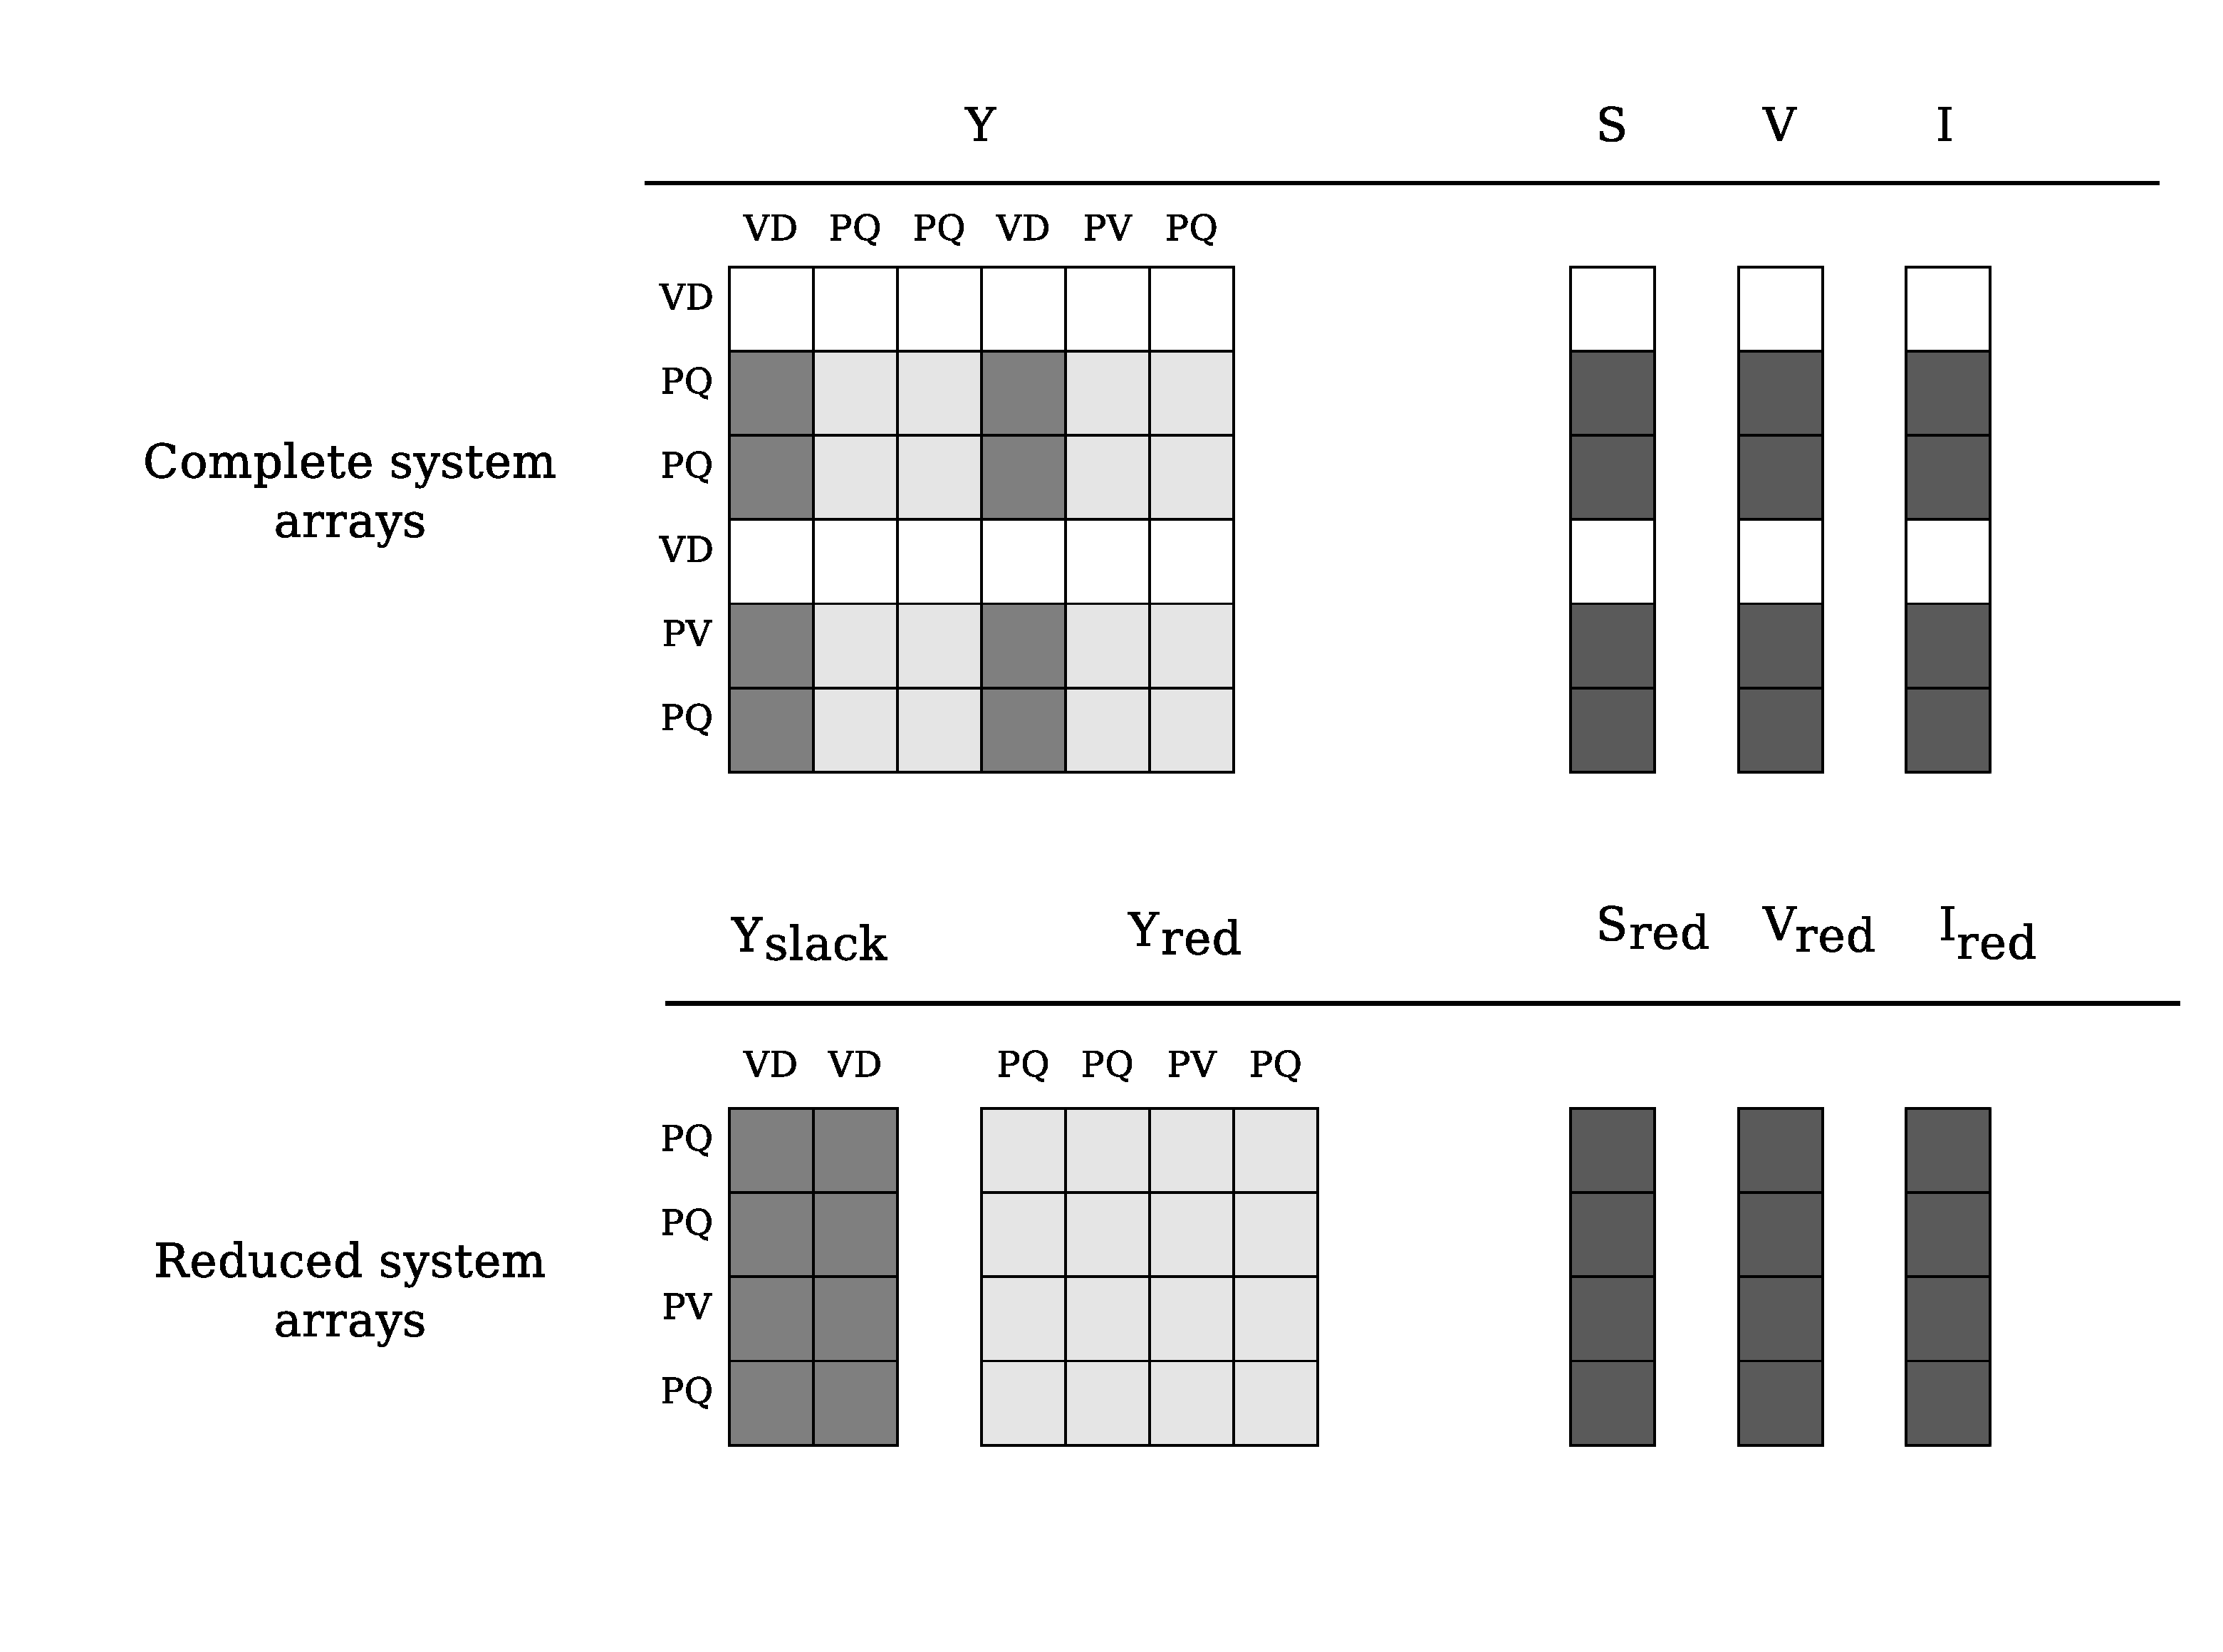
\includegraphics[width=0.85\linewidth]{img/Matrix_reduction.eps}
	\caption{Matrix reduction (VD: Slack, PV: Voltage controlled, PQ: Power controlled)}
	\label{fig:Matrix_reduction}
\end{figure}

%# Decompose the voltage in angle and magnitude
%Va_ref = angle(V0[ref])  # we only need the angles at the slack nodes
%Vm = npabs(V0)
%
%# initialize result vector
%Va = empty(len(V0))
%
%# reconvert the pqpv vector to a matrix so that we can call numpy directly with it
%pvpq_ = matrix(pvpq)
%
%# Compile the reduced imaginary impedance matrix
%Bpqpv = Ybus.imag[pvpq_.T, pvpq_]
%Bref = Ybus.imag[pvpq_.T, ref]
%
%# compose the reduced power injections
%# Since we have removed the slack nodes, we must account their influence as injections Bref * Va_ref
%Pinj = Sbus[pvpq].real - Bref * Va_ref + Ibus[pvpq].real
%
%# update angles for non-reference buses
%Va[pvpq] = spsolve(Bpqpv, Pinj)
%Va[ref] = Va_ref
%
%# re assemble the voltage
%V = Vm * exp(1j * Va)
%
%# compute the calculated power injection and the error of the voltage solution
%Scalc = V * conj(Ybus * V - Ibus)
%
%# compute the power mismatch between the specified power Sbus and the calculated power Scalc
%mis = Scalc - Sbus  # complex power mismatch
%F = r_[mis[pv].real, mis[pq].real, mis[pq].imag]  # concatenate again
%
%# check for convergence
%normF = linalg.norm(F, Inf)

\begin{equation}
\textbf{P} = Re(\textbf{S}_{red}) + (- Im(\textbf{Y}_{slack}) \cdot angle(\textbf{V}_{slack}) + Re(\textbf{I}_{red})) \cdot |\textbf{V}_{red}|
\label{dc_power_injections}
\end{equation}

The equation \ref{dc_power_injections} computes the DC power injections as the sum of the different factors mentioned:

\begin{enumerate}
	\item $Re(\textbf{S}_{red})$: Real part of the reduced power injections.
	\item $Im(\textbf{Y}_{slack}) \cdot angle(\textbf{V}_{slack}) \cdot |v_{red}|$: Currents that appear by removing the slack nodes while keeping their influence, multiplied by the voltage module to obtain power.
	\item $Re(\textbf{I}_{red}) \cdot |v_{red}|$: Real part of the grid reduced current injections, multiplied by the voltage module to obtain power.
\end{enumerate}

Once the power injections are computed, the new voltage angles are obtained by:

\begin{equation}
\textbf{V}_{angles} = Im(\textbf{Y}_{red})^{-1} \times \textbf{P}
\end{equation}

The new voltage is then:
\begin{equation}
\textbf{V}_{red} = |\textbf{V}_{red}| \cdot e^{1j \cdot  \textbf{V}_{angles}}
\end{equation}

This method usually produces a solution with a large power mismatch. That is to be expected because the method is an oversimplification with no iterative convergence criteria, just a straight forward set of operations.


\section{Linear AC power flow}

The AC linear approximation is a much more convenient linearisation of the power flow equation, because it provides the voltage module and angle. This procedure is great for real time applications such as large grids SCADA applications.

Using the formulation presented in \cite{rossoni2016linearized}, we obtain a way to solve circuits in one shot (without iterations) with quite positive results for a linear approximation.

\begin{equation}
\begin{bmatrix}
A_{11} & A_{12} \\
A_{21} & A_{22} \\
\end{bmatrix}
\times
\begin{bmatrix}
\Delta \theta\\
\Delta |V|\\
\end{bmatrix}
=
\begin{bmatrix}
Rhs_1\\
Rhs_2\\
\end{bmatrix}
\end{equation}

Where:
\begin{itemize}
	\item $A_{11} = -Im\left(Y_{series}[pqpv, pqpv]\right)$
	\item $A_{12} = Re\left(Y_{bus}[pqpv, pq]\right)$
	\item $A_{21} = -Im\left(Y_{series}[pq, pqpv]\right)$
	\item $A_{22} = -Re\left(Y_{bus}[pq, pq]\right)$
	\item $Rhs_1 = Re(S[pqpv])$
	\item $Rhs_2 = Im(S[pq])$\newline
\end{itemize}

Here, $Y_{bus}$ is the normal circuit admittance matrix and $Y_{series}$ is the admittance matrix formed with only series elements of the $\pi$ model, this is, neglecting all the shunt admittances.

Solving the vector $[\Delta \theta + 0, \Delta |V| + 1]$ we get $\theta$ for the pq and pv nodes and $|V|$ for the pq nodes.\newline

%For equivalence with the paper:\newline
%
%\begin{itemize}
%	\item $-B' = -Im(Y_{series}[pqpv, pqpv])$
%	\item $G = Re(Y_{bus}[pqpv, pq])$
%	\item $-G' = -Im(Y_{series}[pq, pqpv])$
%	\item $-B = -Re(Y_{bus}[pq, pq])$\newline
%\end{itemize}

The solution obtained has a lower mismatch than the DC approximation usually in the order of $0.1$ p.u. which is acceptable for a linear method. The error is lower because the voltage module is also computed.

\section{Holomorphic embedding}

First introduced by Antonio Trias in 2012 \cite{TriasHELM}, promises to be a non-divergent power flow method. Trias originally developed a version with no voltage controlled nodes (PV), in which the convergence properties are excellent. 

The version programmed in the file \verb|HELM.py| has been adapted from the master thesis of Muthu Kumar Subramanian at the Arizona State University (ASU) \cite{subramanian2014application}. This version includes a formulation of the voltage controlled nodes. My experience indicates that the introduction of the PV control deteriorates the convergence properties of the holomorphic embedding method. However, in many cases, it is the best approximation to a solution. especially when Newton-Raphson does not provide one.


\subsection{Concepts}

All the power flow algorithms until the HELM method was introduced were iterative and recursive. The helm method is iterative but not recursive. A simple way to think of this is that traditional power flow methods are exploratory, while the HELM method is a planned journey. In theory the HELM method is superior, but in practice the numerical degeneration makes it less ideal.

The fundamental idea of the recursive algorithms is that given a voltage initial point (1 p.u. at every node, usually) the algorithm explores the surroundings of the initial point until a suitable voltage solution is reached or no solution at all is found because the initial point is supposed to be "far" from the solution.

On the HELM methods, we form a "curve" that departures from a known mathematically exact solution that is obtained from solving the grid with no power injections. This is possible because with no power injections, the grid equations become linear and straight forward to solve. The arriving point of the "curve" is the solution that we want to achieve. That "curve" is best approximated by a Pad\'e approximation. To compute the Pad\'e approximation we need to compute the coefficients of the unknown variables, in our case the voltages (and possibly the reactive powers at the PV nodes).

The HELM formulation consists in the derivation of formulas that enable the calculation of the coefficients of the series that describes the "curve" from the mathematically know solution to the unknown solution. Once the coefficients are obtained, the Pad\'e approximation computes the voltage solution at the "end of the curve", providing the desired voltage solution. The more coefficients we compute the more exact the solution is (this is true until the numerical precision limit is reached).\newline 


All this sounds very strange, but it works ;)\newline 


If you want to get familiar with this concept, you should read about the homotopy concept. In practice the continuation power flow does the same as the HELM algorithm, it takes a known solution and changes the loading factors until a solution for another state is reached.

\subsection{Fundamentals} \label{helm_fundamentals}

The fundamental equation that defines the power flow problem is:
\begin{equation}
\textbf{S} = \textbf{V} \times (\textbf{Y} \times \textbf{V})^*
\end{equation}

Most usefully represented like this:


\begin{equation}
{\textbf{Y} \times \textbf{V}} = \left(\frac{\textbf{S}}{\textbf{V}}\right)^* 
\label{base_eq}
\end{equation}


The holomorphic embedding is to insert a "travelling" parameter $\alpha$, such that for $\alpha=0$ we have an mathematically exact solution of the problem (but not the solution we're looking for...), and for $\alpha=1$ we have the solution we're looking for. The other thing to do is to represent the variables to be computed as McLaurin series. Let's go step by step.\newline

For $\alpha=0$ we say that $S=0$, in this way the equation \ref{base_eq} becomes linear, and its solution is mathematically exact. But for that to be useful in our case we need to split the admittance matrix $Y$ into $Y_{series}$ and $Y_{shunt}$. $Y_{shunt}$ is a diagonal matrix, so it can be expressed as a vector instead (no need for matrix-vector product).

\begin{equation}
\textbf{Y}_{series} \times \textbf{V} = \left(\frac{\textbf{S}}{\textbf{V}}\right)^* - \textbf{Y}_{shunt} \textbf{V}
\label{base_eq_alpha_0}
\end{equation}

This is what will allow us to find the zero "state" in the holomorphic series calculation. For $\alpha=1$ we say that $S=S$, so we don't know the voltage solution, however we can determine a path to get there:

\begin{equation}
{\textbf{Y }\times \textbf{V}( \alpha )} = \left(\frac{ \alpha\textbf{S}}{\textbf{V}( \alpha )}\right)^* - \alpha \textbf{Y}_{shunt} \times \textbf{V}( \alpha ) = \frac{ \alpha\textbf{S}^*}{\textbf{V}( \alpha )^*} - \alpha \textbf{Y}_{shunt} \textbf{V}( \alpha )
\label{base_eq_embedded}
\end{equation}

Wait, what?? did you just made this stuff up??, well so far my reasoning is:
\begin{itemize}
	\item The voltage $\textbf{V}$ is what I have to convert into a series, and the series depend of $\alpha$, so it makes sense to say that $\textbf{V}$, as it is dependent of $\alpha$, becomes $\textbf{V}(\alpha)$.
	
	\item Regarding the $\alpha$ that multiplies $\textbf{S}$, the amount of power ($\alpha \textbf{S}$) is what I vary during the \textit{travel} from $\alpha=0$ to $\alpha=1$, so that is why $\textbf{S}$ has to be accompanied by the \textit{traveling} parameter $\alpha.$
	
	\item In my opinion the $\alpha$ $\textbf{Y}_{shunt}$ is to provoke the first voltage coefficients to be one.  $\textbf{Y}_{series} \times \textbf{V}[0] = 0$, makes $V[0]=1$. This is essential for later steps (is a condition to be able to use Pad\'e). \newline
\end{itemize}

The series are expressed as McLaurin equations:

\begin{equation}
V(\alpha) = \sum_{n}^{\infty} V_n \alpha ^n
\label{eq:McLaurinV}
\end{equation}

\subsection{Holomorphicity check}
	
	There's still something to do. The magnitude $\left(\textbf{V}( \alpha )\right)^*$ has to be converted into $\left(\textbf{V}( \alpha^* )\right)^*$. This is done in order to make the function be holomorphic. The holomorphicity condition is tested by the Cauchy-Riemann condition, this is $\partial \textbf{V} / \partial \alpha^* = 0$, let's check that:
	
	\begin{equation}
	\partial \left(\textbf{V}( \alpha )^*\right) / \partial \alpha^*  = \partial \left(\sum_{n}^{\infty} V_n^* (\alpha ^n)^*\right) / \partial \alpha^*  = \sum_{n}^{\infty} \alpha ^n V_n^* (\alpha ^{n-1})^*
	\end{equation} 
	Which is not zero, obviously. Now with the proposed change:
	
	\begin{equation}
	\partial \left( \textbf{V}( \alpha^* )\right)^* / \partial \alpha^*  = \partial \left(\sum_{n}^{\infty} \textbf{V}_n^* \alpha ^n \right) / \partial \alpha^*  = 0
	\end{equation} 
	
	Yay!, now we're mathematically happy, since this stuff has no effect in practice because our $\alpha$ is not going to be a complex parameter, but for sake of being correct the equation is now:
	
	\begin{equation}
	{\textbf{Y}_{series}\times \textbf{V}( \alpha )} = \frac{ \alpha\textbf{S}^*}{\textbf{V}^*( \alpha^* )} - \alpha \textbf{Y}_{shunt} \textbf{V}( \alpha )
	\label{base_eq_embedded2}
	\end{equation}
	



The fact that $\textbf{V}^*( \alpha^* )$ is dividing is problematic. We need to express it as its inverse so it multiplies instead of divide.

\begin{equation} 
\frac{1}{\textbf{V}( \alpha)} = \textbf{W}( \alpha ) \longrightarrow \textbf{W}( \alpha ) \textbf{V}( \alpha) = 1 \longrightarrow \sum_{n=0}^{\infty}{\textbf{W}_n \alpha^n}  \sum_{n=0}^{\infty}{\textbf{V}_n \alpha^n} = 1
\end{equation}

Expanding the series and identifying terms of $\alpha$ we obtain the expression to compute the inverse voltage series coefficients:

\begin{equation}
\textbf{W}_n =
\left\{
\begin{array}{ll}
\mathlarger{\frac{1}{\textbf{V}_0}}, \quad n=0\\
\mathlarger{-\frac{\mathlarger{\sum_{k=0}^{n}\textbf{W}_k \textbf{V}_{n-k}}}{\textbf{V}_0}}, \quad n>0
\end{array}
\right.
\end{equation}


Now, the equation \ref{base_eq_embedded2} is:

\begin{equation}
{\textbf{Y}_{series}\times \textbf{V}( \alpha )} = \alpha\textbf{S}^* \cdot \textbf{W}( \alpha)^*  - \alpha \textbf{Y}_{shunt} \textbf{V}( \alpha )
\label{base_eq_embedded3}
\end{equation}

Substituting the series by their McLaurin expressions:

\begin{equation}
{\textbf{Y}_{series}\times \sum_{n=0}^{\infty}{\textbf{V}_n \alpha^n}} = \alpha\textbf{S}^* \left(\sum_{n=0}^{\infty}{\textbf{W}_n \alpha^n}\right)^*  - \alpha \textbf{Y}_{shunt} \sum_{n=0}^{\infty}{\textbf{V}_n \alpha^n}
\label{base_eq_embedded4}
\end{equation}

Expanding the series an identifying terms of $\alpha$ we obtain the expression for the voltage coefficients:

\begin{equation}
\textbf{V}_n =
\left\{
\begin{array}{ll}
\mathlarger{0}, \quad n=0\\
\mathlarger{\textbf{S}^* \textbf{W}^*_{n-1} - Y_{shunt} \textbf{V}_{n-1} }, \quad n>0
\end{array}
\right.
\end{equation}

This is the HELM fundamental formula derivation for a grid with no voltage controlled nodes (no PV nodes). Once a sufficient number of coefficients are obtained, we still need to use the Pad\'e approximation to get voltage values out of the series.


In the previous formulas, the number of the bus has not been explicitly detailed. All the $\textbf{V}$ and the $\textbf{W}$ are matrices of dimension $n \times nbus$ (number of coefficients by number of buses in the grid) This structures are depicted in the figure \ref{fig:CoefficientsStructure}. For instance $\textbf{V}_n$ is the $n^{th}$ row of the coefficients structure $\textbf{V}$.


\begin{figure}[h]
	\centering
	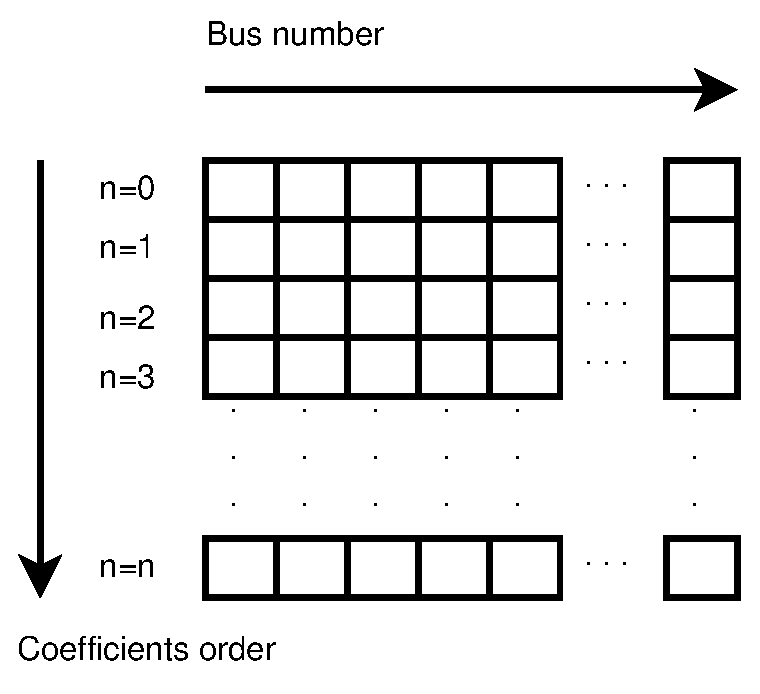
\includegraphics[width=0.4\linewidth]{img/CoefficientsStructure.eps}
	\caption{Structure of the coefficients}
	\label{fig:CoefficientsStructure}
\end{figure}

\subsection{Pad\'e approximation}

The equation \ref{eq:McLaurinV} provides us with an expression to obtain the voltage from the coefficients, knowing that for $\alpha=1$ we get the final voltage results. So, why do we need any further operation?, and what is this Pad\'e thing?

Well, it is true that the equation \ref{eq:McLaurinV} provides an approximation of the voltage by means of a series (this is similar to a Taylor approximation), but in practice, the approximation might provide a wrong value for a given number of coefficients. The Pad\'e approximation accelerates the convergence of any given series, so that you get a more accurate result with less coefficients. This means that for the same series of voltage coefficients, using the equation \ref{eq:McLaurinV} could give a completely wrong result, whereas by applying Pad\'e to those coefficients one could obtain a fairly accurate result.

The Pad\'e approximation is a rational approximation of a function. In our case the function is $\textbf{V}(\alpha)$, represented by the coefficients structure $\textbf{V}$. The approximation is valid over a small domain of the function, in our case the domain is $\alpha=[0,1]$. The method requires the function to be continuous and differentiable for $\alpha=0$. Hence the Cauchy-Riemann condition. And yes, our function meets this condition, we tested it before.

\paragraph{Pad\'e approximation algorithm}

The canonical Pad\'e algorithm for our problem is described by:

\begin{equation}
Voltage\_value\_approximation = \frac{P_N(\alpha)}{Q_M(\alpha)} \quad \forall \alpha \in [0,1]
\label{eq:pade_apprx}
\end{equation}

Here $N=M=n/2$, where $n$ is the number of available voltage coefficients, which has to be an even number to be exactly divisible by $2$. $P$ and $Q$ are polynomials which coefficients $p_i$ and $q_i$ must be computed. It turns out that if we make the first term of $Q_M(\alpha)$ be $q_0=1$, the function to be approximated is given by the McLaurin expression (What a happy coincidence!)
\begin{equation}
P_N(\alpha) = p_0 + p_1\alpha + p_2\alpha^2 + ... + p_N\alpha^N
\end{equation}

\begin{equation}
Q_M(\alpha) = 1 + q_1\alpha + q_2\alpha^2 + ... + q_M\alpha^M
\end{equation}



The problem now boils down to find the coefficients $q_i$ and $p_i$. This is done by solving two systems of equations. The first one to find $q_i$ which does not depend on $p_i$, and the second one to get $p_i$ which does depend on $q_i$.

\textbf{First linear system}: The only unknowns are the $q_i$ coefficients.

\begin{equation}
\begin{matrix}
q_M V_{N-M+1} + q_{M-1}V_{N-M+2}+...+q_1V_N = 0\\
q_M V_{N-M+2} + q_{M-1}V_{N-M+3}+...+q_1V_{N+1} = 0\\
...\\
q_M V_{N} + q_{M-1}V_{N+1}+...+q_1V_{N+M+1} + V_{N+M} = 0\\
\end{matrix}
\end{equation}

\textbf{Second linear System}: The only unknowns are the $p_i$ coefficients.
\begin{equation}
\begin{matrix}
V_0 - p_0=0\\
q_1V_0 + V_1  p_1=0\\
q_2V_0 + q_1V_1+V_2-p_2=0\\
q_3V_0 + q_2V_1 + q_1V_2 + V_3 - p_3 = 0\\
...\\
q_MV_{N-M} + q_{M-1}V_{N-M+1} + ... + +V_N - p_N=0
\end{matrix}
\end{equation}

Once the coefficients are there, you would have defined completely the polynomials $P_N(\alpha)$ and $Q_M(\alpha)$, and it is only a matter of evaluating the equation \ref{eq:pade_apprx} for $\alpha=1$.\newline


This process is done for every column of coefficients $\textbf{V}=\{V_0, V_1,V_2,V_3, ...,V_n\}$ of the structure depicted in the figure \ref{fig:CoefficientsStructure}. This means that we have to perform a Pad\'e approximation for every node, using the one columns of the voltage coefficients per Pad\'e approximation.

\paragraph{Wynn's Pad\'e approximation algorithm}

Wynn published a paper in 1969 where he proposed a simple calculation method to obtain the Pad\'e approximation. This method is based on a table. Weniger in 1989 publishes his thesis where a faster version of Wynn's algorithm is provided in Fortran code. 


One of the advantages of this method over the canonical Pad\'e approximation implementation is that it can be used for every iteration. In the beginning I thought it would be faster but it turns out that it is not faster since the amount of computation increases with the number of coefficients, whereas with the canonical implementation the order of the matrices does not grow dramatically and it is executed the half of the times.

On top of that my experience shows that the canonical implementation provides a more consistent convergence.

Anyway, both implementations are there to be used in the code.




\subsection{Formulation with PV nodes}

The section \ref{helm_fundamentals} introduces the canonical HELM algorithm. That algorithm does not include the formulation of PV nodes.
Other articles published on the subject feature PV formulations that work more or less to some degree. The formulation below is a formulation corrected by myself from a formulation contained here \cite{liu2017online}, which does not work as published, hence the correction.



\paragraph{Embedding}

The following embedding equations are proposed instead of the canonical HELM equations from section \ref{helm_fundamentals}.

For Slack nodes:
\begin{equation}
V(\alpha) = V^{SP} \quad \forall \alpha=0
\end{equation}

For PQ nodes:
\begin{equation}
\left\{
\begin{array}{ll}
\textbf{Y} \times \textbf{V}(\alpha) = 0 \quad \quad \quad \quad \forall \alpha=0\\
\mathlarger{\textbf{Y} \times \textbf{V}(\alpha) = \frac{\alpha \textbf{S}}{\textbf{V}^*(\alpha^*)}} \quad \forall \alpha>0
\end{array}
\right.
\end{equation}

For PV nodes:

\begin{equation}
\left\{
\begin{array}{ll}
\mathlarger{\textbf{Y} \times \textbf{V}(\alpha) = \frac{ \textbf{S}}{\textbf{V}^*(\alpha^*)}} \quad \forall \alpha=0\\
\mathlarger{\textbf{Y} \times \textbf{V}(\alpha) = \frac{ \textbf{S} - j \textbf{Q}(\alpha)}{\textbf{V}^*(\alpha^*)}} \quad \forall \alpha>0
\end{array}
\right.
\end{equation}

\begin{equation}
\left\{
\begin{array}{ll}
V(\alpha)V^*(\alpha^*) = |V_0|^2\quad \quad \quad \quad \forall \alpha=0\\
V(\alpha)V^*(\alpha^*) = |V_0|^2 + (|V^{SP}|^2-|V_0|^2) \quad \forall \alpha>0
\end{array}
\right.
\end{equation}




This embedding translates into the following formulation:

\paragraph{Step 1}

The formulas are adapted to exemplify a 3-bus system where the bus1 is a slack, the bus 2 is PV and the bus 3 is PQ. This follows the example of the Appendix A of \cite{liu2017online}.

\vspace{1cm}

Compute the initial no-load solution ($n=0$):

\begin{equation}
\begin{bmatrix}
1 & 0 & 0 & 0 & 0 & 0\\
0 & 1 & 0 & 0 & 0 & 0\\
G_{21} & -B_{21} & G_{22} & -B_{22} & G_{23} & -B_{23}\\
B_{21} & G_{21}  & B_{22} & G_{22}  & B_{23} & G_{23}\\
G_{31} & -B_{31} & G_{32} & -B_{32} & G_{33} & -B_{33}\\
B_{31} & G_{31}  & B_{32} & G_{32}  & B_{33} & G_{33}\\
\end{bmatrix}
\times
\begin{bmatrix}
V[n]_{re, 1}\\
V[n]_{im, 1}\\
V[n]_{re, 2}\\
V[n]_{im, 2}\\
V[n]_{re, 3}\\
V[n]_{im, 3}\\
\end{bmatrix}
=
\begin{bmatrix}
V^{SP}_{re, 1}\\
V^{SP}_{im, 1}\\
0\\
0\\
0\\
0\\
\end{bmatrix}
\quad \forall n = 0
\end{equation}

Form the solution vector $\textbf{V}[n]$ you can compute the buses calculated power and then get the reactive power at the PV nodes to initialize $\textbf{Q}[0]$:

\begin{equation}
\textbf{S} = \textbf{V}[0] \cdot (\textbf{Y}_{bus} \times \textbf{V}[0])^*
\label{Scalc}
\end{equation}

\begin{equation}
\textbf{Q}_i[0] = Im(\textbf{S}_{i}) \quad \forall i \in PV
\end{equation}

The initial inverse voltage coefficients $\textbf{W}[0]$ are obtained by:

\begin{equation}
W_i[0] = \frac{1}{V_i[0]}  \quad \forall i \in N
\end{equation}

This step is entirely equivalent to find the no load solution using the Z-Matrix reduction.

\paragraph{Step 2}

Construct the system of equations to solve the coefficients of order greater than zero ($n>0$). Note that the matrix is the same as constructed for the previous step, but adding a column and a row for each PV node to account for the reactive power coefficients. In our 3-bus example, there is only one PV node, so we add only one column and one row.

\begin{equation}
\begin{bmatrix}
1 & 0 & 0 & 0 & 0 & 0 & 0\\
0 & 1 & 0 & 0 & 0 & 0 & 0\\
G_{21} & -B_{21} & G_{22} & -B_{22} & G_{23} & -B_{23} & W[0]_{im}\\
B_{21} & G_{21}  & B_{22} & G_{22}  & B_{23} & G_{23} & W[0]_{re}\\
G_{31} & -B_{31} & G_{32} & -B_{32} & G_{33} & -B_{33} & 0\\
B_{31} & G_{31}  & B_{32} & G_{32}  & B_{33} & G_{33} & 0\\
0 & 0 & V[0]_{re} & V[0]_{im} & 0 & 0 & 0\\
\end{bmatrix}
\times
\begin{bmatrix}
V[n]_{re, 1}\\
V[n]_{im, 1}\\
V[n]_{re, 2}\\
V[n]_{im, 2}\\
V[n]_{re, 3}\\
V[n]_{im, 3}\\
Q_2[n]\\
\end{bmatrix}
=
\begin{bmatrix}
0\\
0\\
f2_{re}\\
f2_{im}\\
f1_{re}\\
f1_{im}\\
\epsilon[n]\\
\end{bmatrix}
\quad \forall n > 0
\label{lin_sys_2}
\end{equation}

Where:

\begin{equation}
f1 = S^*_i \cdot W^*_i[n-1] \quad \forall i \in PQ
\end{equation}

\begin{equation}
f2 = P_i \cdot W^*_i[n-1] + conv(n, Q_i, W^*_i) \quad \forall i \in PV
\end{equation}

\begin{equation}
\epsilon[n] = \delta_{n1} \cdot \frac{1}{2} \left(|V_i^SP|^2 - |V_i[0]|^2\right) - \frac{1}{2} conv(n, V_i, V_i^*)  \quad \forall i \in PV, n > 0
\end{equation}

The convolution $conv$ is defined as:

\begin{equation}
conv(n, A, B) = \sum_{m=0}^{n-1} A[m] \cdot B[n-m]
\end{equation}

The system matrix ($A_{sys}$) is the same for all the orders of $n>0$, therefore we only build it once, and we factorize it to solve the subsequent coefficients.

After the voltages $\textbf{V}[n]$ and the reactive power at the PV nodes $Q[n]$ is obtained solving the linear system (eq \ref{lin_sys_2}), we must solve the inverse voltage coefficients of order $n$ for all the buses:

\begin{equation}
W_i[n] = \frac{- \mathlarger{\sum_{m=0}^{n}W_i[m] \cdot V_i[n-m]} }{V_i[0]} \quad  \forall i \in N, n>0
\end{equation}


\paragraph{Step 3}

Repeat step 2 until a sufficiently low error is achieved or a maximum number of iterations (coefficients).


The error is computed by comparing the calculated power $\textbf{S}$ (eq \ref{Scalc}) with the specified power injections $\textbf{S}^{SP}$:

\begin{equation}
mismatch = \textbf{S} - \textbf{S}^{SP}
\end{equation}

\begin{equation}
error = |mismatch|_\infty = max(abs(mismatch))
\end{equation}



\section{Post voltage solution: Compute the power flows} \label{post_voltage_solution}

Ironically, what is called the power flow problem does not compute the power flows in the branches of a grid. It computes the node voltages. In this section we explain how to compute the current and power that flows through the grid branches using a given voltage solution vector.

First we compute the branches per unit currents:

\begin{equation}
{\textbf{I}_f = \textbf{Y}_f \times \textbf{V}}
\end{equation}

\begin{equation}
{\textbf{I}_t = \textbf{Y}_t \times \textbf{V}}
\end{equation}


These are matrix-vector multiplications. The result is the per unit currents flowing through a branch seen from the \textit{from} bus or from the \textit{to} bus.


Then we compute the power values:

\begin{equation}
{\textbf{S}_f = \textbf{V}_f \cdot \textbf{I}_f^*}
\end{equation}

\begin{equation}
{\textbf{S}_t = \textbf{V}_t \cdot \textbf{I}_t^*}
\end{equation}

These are element-wise multiplications, resulting in the per unit power flowing through a branch seen from the \textit{from} bus or from the \textit{to} bus.

Now we can compute the losses in MVA as:

\begin{equation}
{\textbf{losses} = |\textbf{S}_f - \textbf{S}_t| \cdot Sbase}
\end{equation}

And also the branches loading in per unit as:
\begin{equation}
{\textbf{loading} = \frac{max(|\textbf{S}_f|, |\textbf{S}_t|) \cdot Sbase}{ \textbf{rate}}}
\end{equation}

The variables are:

\begin{itemize}
	\item $\textbf{Y}_f, \textbf{Y}_t$: \textit{From} and \textit{To} bus-branch admittance matrices, see section \ref{Y_calculation}.
	\item $\textbf{I}_f$: Array of currents at the \textit{from} buses in p.u.
	\item $\textbf{I}_t$: Array of currents at the \textit{to} buses in p.u.
	\item $\textbf{S}_f$: Array of powers at the \textit{from} buses in p.u.
	\item $\textbf{S}_t$: Array of powers at the \textit{to} buses in p.u.
	\item $\textbf{V}_f$: Array of voltages at the \textit{from} buses in p.u.
	\item $\textbf{V}_t$: Array of voltages at the \textit{to} buses in p.u.
	\item $\textbf{rate}$: Array of branch ratings in MVA.
\end{itemize}



%-------------------------------------------------------------------------------
%	CHAPTER Short-circuit
%-------------------------------------------------------------------------------
\chapter{Optimal power flow (OPF)}

The optimal power flow are a set of problems which implementation call for the usage of MIP solvers (Mixed-Integer Programming solvers). However that is not a hard requirement and other methods might be used such as genetic algorithms, convex solvers, etc.


\subsection{DC optimal power flow}

The power flow problem consists in finding the voltages of a circuit given the nodal power injections and the circuit admittances. The power flow equation in summation expression is:

\begin{equation}
S_i=V_i \sum_j^{nodes} \left(Y_{ij} \cdot V_j\right) ^* \quad  \forall i \in nodes
\end{equation}

The non-vectorized expression is of use now, because the MIP formulation of the OPF problem does not allow vectorization usually.

The optimal power flow problem consists in finding the generators power injections that supply the demand and the losses while minimizing the grid violations (Voltages out of bounds and branch flows limits). Here we are going to adapt the formulation developed in the previous chapter in order to accommodate the generators dispatch.

Minimize the generators dispatch cost, including the cost of the slack generators:

\begin{equation}
min: \sum_i^{Generators+Slack} cost_i \cdot PG_i 
\end{equation}

ST: 
Generator limits must be within boundaries (include the slack generator as well)
\begin{equation}
PG_i^{min} \leq PG_i \leq PG_i^{max}
\end{equation}

\marginnote{When traversing the matrix B, try to avoid two for loops, dealing with B as if it was dense because it is not. Ideally B should be in CSC format. Then traversing B in sparse mode is several orders of magnitude faster.}

The voltages must satisfy the power balance in every PQ and PV node.
\begin{equation}
PG_i - PD_i=\sum_j^{PQPV} B_{ij} \cdot \theta_j  \quad  \forall i \in PQPV
\end{equation}



The slack voltage angles are set to zero.
\begin{equation}
\theta_k=0   \quad \forall k \in Slack
\end{equation}


The branch flows must be within limits.

\begin{equation}
-F_{ij}^{max} \leq B_{ij}⋅(\theta_i - \theta_j) \leq F_{ij}^{max}
\end{equation}


This is reformulated as:

\begin{equation}
 B_{ij}⋅(\theta_i - \theta_j) \leq F_{ij}^{max}
\end{equation}

\begin{equation}
 B_{ij}⋅(\theta_j - \theta_i) \leq F_{ij}^{max}
\end{equation}

Set the slack generator power:

\begin{equation}
PG_i - PD_i=\sum_j^{nodes} B_{ij} \cdot \theta_j  \quad  \forall i \in Slack
\end{equation}

\begin{itemize}
	\item $P_i$: Active power injection at the node i.
	\item $B$: Susceptance matrix. It is the imaginary part of the circuit admittance matrix.
	\item $\theta$: Voltage angles in radians.
	\item $PQPV$: Set of the non-slack nodes.
	
	\item $Slack$: Set of the slack nodes.
\end{itemize}

There are plenty of other formulations that feature ramps, multiple periods and the modelling of other devices.
For an overview of such methods see \cite{taylor2015convex}.

%-------------------------------------------------------------------------------
%	CHAPTER Time series power flow
%-------------------------------------------------------------------------------
\chapter{Time series power flow}

The time series power flow is nothing more than power flows executed sequentially for series of profiles of load and generation. The usage of this simulation is to inspect how does the voltage and loading behave given a profile of the load and generation of the grid.

\begin{marginfigure}
	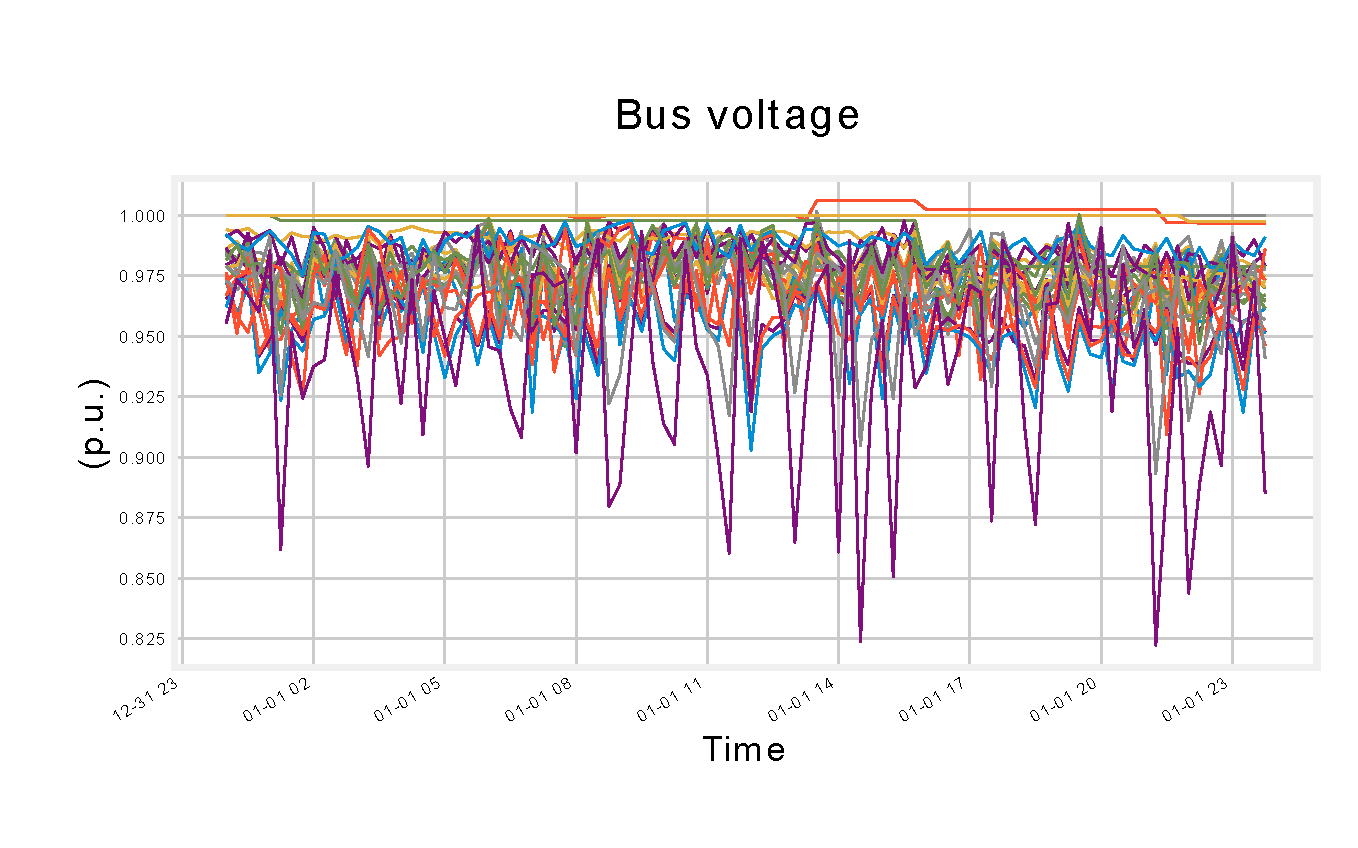
\includegraphics[width=\linewidth]{img/Time_series.eps}
	\caption{Example of voltage results for a time series simulation.}
	\label{fig:time_series}
\end{marginfigure}

\paragraph{Algorithm}

\begin{enumerate}
	\item Compile the load and generation profiles
	
	\item initialize the control variables. $t=0$.
	
	\item for each profile step:
	
	\begin{itemize}
		\item Pick grid load state at $t$, and for the injection vectors $S$ and $I$.
		
		\item Run a power flow simulation with those injection vectors and collect the voltage result $V$.
		
		\item Process the time dependent devices control. i.e Batteries state of charge.
		
	\end{itemize}

	\item End.
\end{enumerate}


%-------------------------------------------------------------------------------
%	CHAPTER Stochastic power flow
%-------------------------------------------------------------------------------
\chapter{Stochastic power flow}

The stochastic power flow is a simulation mode that runs power flows for several randomly generated states of the grid. Those states are defined by combinations of load and generation random samples and a fix connectivity state. The goal is to obtain the probability distribution of the voltages and the branch loading given the probability distribution of the load and the generation. 

$$
CDF_{voltage} = f(CDF_{power})
$$

Mathematically speaking, we want to obtain the cumulative frequency distribution (CDF) of the voltages, as a function of the CDF of the power injections. The transformation function chosen is the power flow.

Varying the connectivity is definitely possible but it will interfere with the purpose of this simulation. If there is the need to vary the connectivity, then it is recommended to run a stochastic simulation for each connectivity state.

%%%%%%%%%%%%%%%%%%%%%%%%%%%%%%%%%%%%%%%%%%%%%%%%%%%%%%%%%%%%%%%%
\section{Cumulative Distribution Function (CDF)}

Usually, one finds that tools model loads and generation with probability distribution functions (PDF) such as the normal or Weibull distributions. In the author's opinion there is a much easier and correct way: To use only data-based cumulative distribution functions (CDF). This allows you to build sampling artefacts from any data source real or theoretical.

\paragraph{Building a CDF}

Suppose that you have recorded load data from a smart meter or any other device. Suppose that there are a thousand values in the record.

To build a CDF:

\begin{itemize}
	\item Sort the records by value, this is the $y$ value from the CDF. $data = sort(records)$
	\item The associated probabilities are an array of equal length. These are given by the expression: $$p_i = \frac{i}{n-1} \quad \forall n > 1, i \in {0..n-1}$$
\end{itemize}

\paragraph{Simple example}

If the records are:
$$
records = [0.2, 0.5, 0.8, 0.3, 0.1, 0.2, 0.3, 0.5, 0.7]
$$

The CDF is:

$$
CDF_{data} = [0.1, 0.2, 0.2, 0.3, 0.3, 0.5, 0.5, 0.7, 0.8]
$$
$$
CDF_{probabilities} = [0, 0.125, 0.25, 0.375, 0.5, 0.625, 0.875, 1.0]
$$

\paragraph{Sampling the CDF}

Once constructed, we can draw infinite samples from the CDF in a very simple way.

First we need to have an interpolation function (linear, quadratic, cubic, spline, ..., at your choice)

Then, We need a uniformly distributed random number generator ($rand$ usually)

With these, we get a new load value from the CDF, by interpolating with a randomly generated probability.

$$
p_{new} = rand(0, 1)
$$

$$
value_{new} = interpolate(CDF_{probabilities}, CDF_{data}, p_{new})
$$

\begin{marginfigure}
	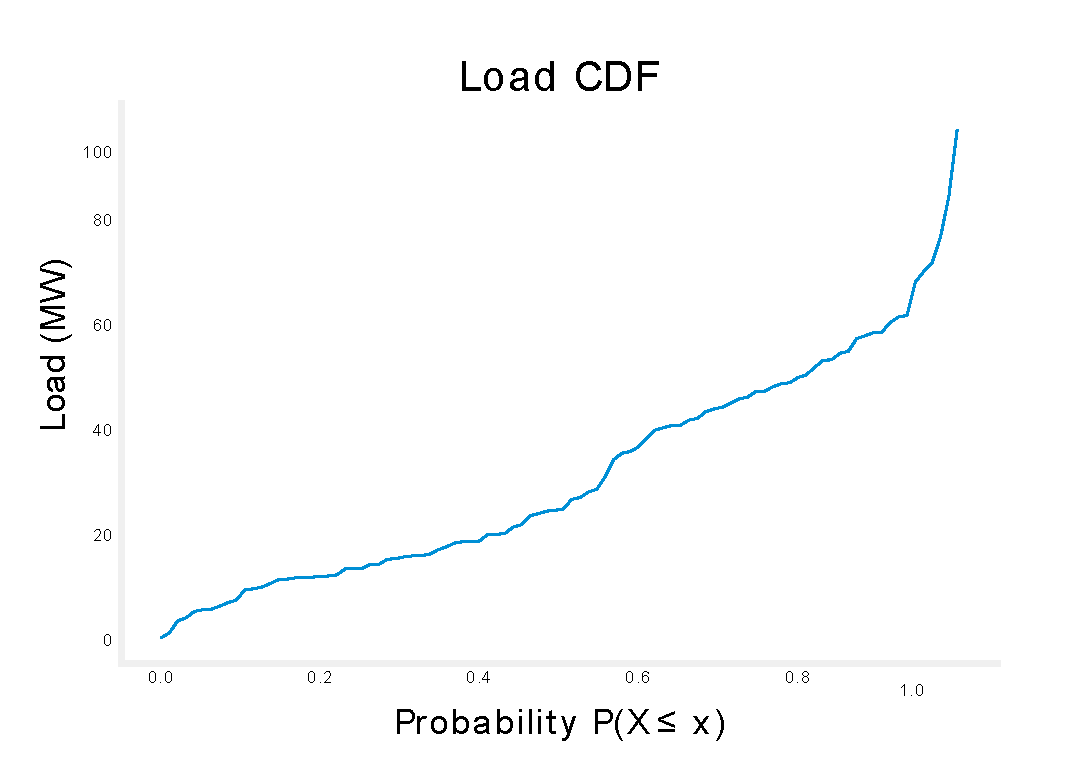
\includegraphics[width=\linewidth]{img/Load_CDF.eps}
	\caption{Example of cumulative distribution function of a load.}
	\label{fig:load_CDF}
\end{marginfigure}

\begin{marginfigure}
	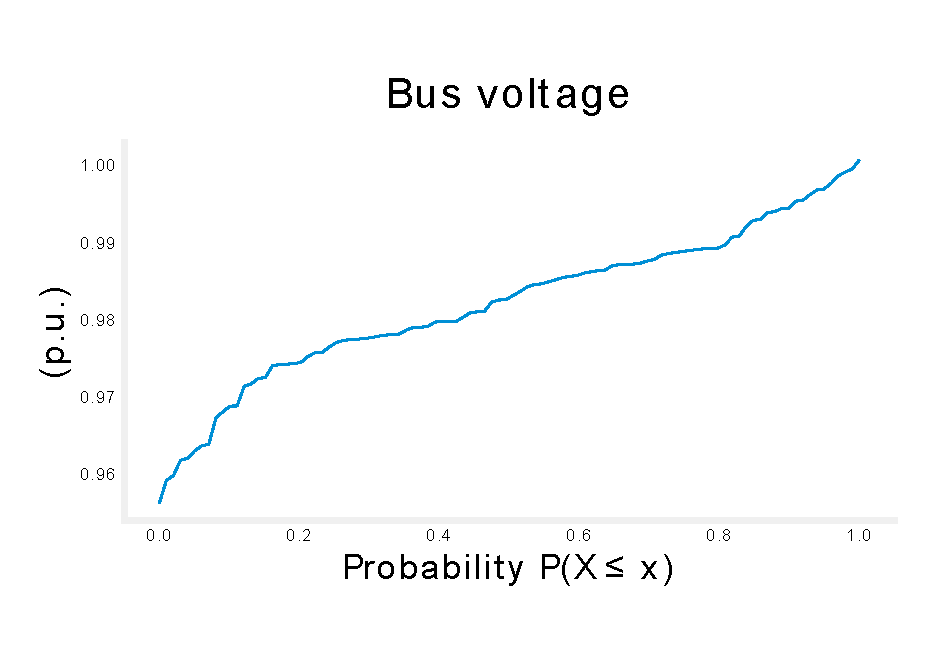
\includegraphics[width=\linewidth]{img/Voltage_CDF.eps}
	\caption{Example of cumulative distribution function of the voltage. This is the Result of a probabilistic power flow.}
	\label{fig:Voltage_CDF}
\end{marginfigure}



%%%%%%%%%%%%%%%%%%%%%%%%%%%%%%%%%%%%%%%%%%%%%%%%%%%%%%%%%%%%%%%%
\section{Monte Carlo}

The Monte Carlo simulation was invented by Stanislaw Ulam and John von Neumann to simulate the diffusion of uranium electrons while developing the nuclear bomb. This very simple algorithm has proven to be an incredibly powerful tool to estimate uncertain behaviours, and it is the de-facto algorithm to simulate stochastic power flows.

The underlying idea is to draw $n$ samples and compute the average. When the average's standard deviation becomes sufficiently small, it indicates that enough samples have been drawn to characterize the system.

In our case, we will draw load and generation samples, evaluate the voltage by running a power flow with those samples and calculate the  voltage mean and standard deviation. When the standard deviation becomes small enough (a tolerance value that we set) we stop sampling. See the figure \ref{fig:Voltage_convergence}.


\begin{marginfigure}
	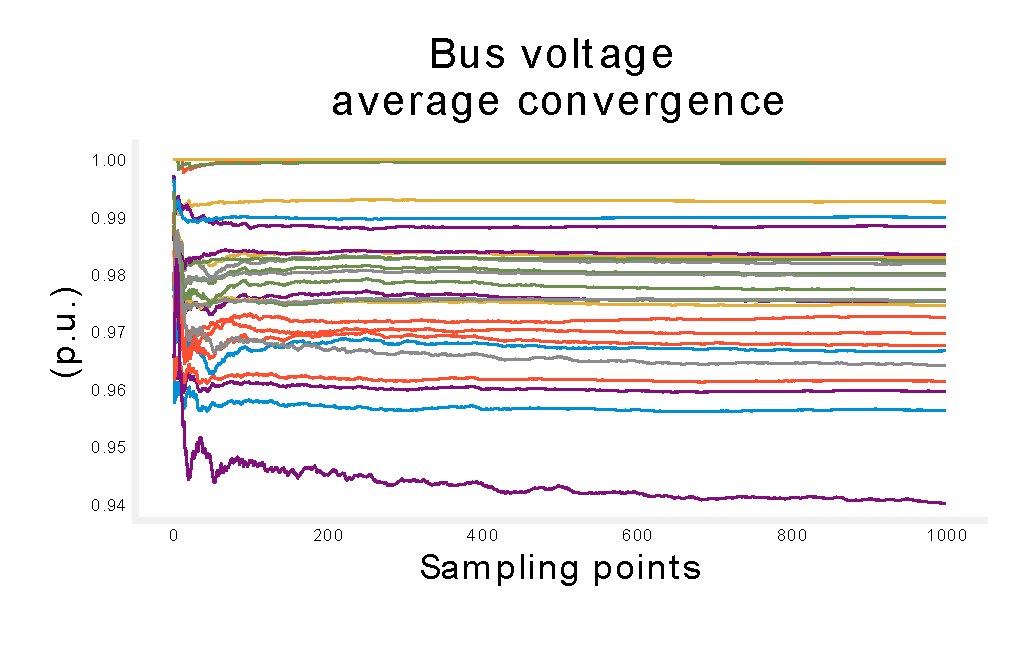
\includegraphics[width=\linewidth]{img/Voltage_convergence.eps}
	\caption{Example of voltage convergence. This is the Result of a probabilistic power flow.}
	\label{fig:Voltage_convergence}
\end{marginfigure}


\paragraph{Algorithm}

\begin{enumerate}
	\item Construct the CDF of all the loads and generators from their profiles of data. For the loads we construct a DSF for the active power and another for the reactive power, for the generators, we only need the CDF for the active power.
	
	\item Initialize control variables: $iterations = 0$, $\textbf{V}_{summation} = 0$
	
	\item While the variance is less than a tolerance value:
	
	\begin{enumerate}
		\item Construct the injection vectors $S$ and $I$, sampling from the CDF.
		
		\item Run a power flow (see chapter \ref{ch:power_flow}) with those arrays and get the voltages vector $\textbf{V}$.
		
		\item Increase the number of iterations: $iterations += 1$
		
		\item Compute the voltages summation: $\textbf{V}_{summation} += \textbf{V}$
		
		\item Compute the voltage average: $\textbf{V}_{mean} = \textbf{V}_{summation} / iterations$
		
		\item Compute the variance: $min((\textbf{V} - \textbf{V}_{mean})^2 / (iterations - 1))$
		
		\item Store all the values that you want to have at the end of the loop.
		
	\end{enumerate}

	\item End.
\end{enumerate}






%%%%%%%%%%%%%%%%%%%%%%%%%%%%%%%%%%%%%%%%%%%%%%%%%%%%%%%%%%%%%%%%
\section{Latin Hypercube}




%-------------------------------------------------------------------------------
%	CHAPTER State estimation
%-------------------------------------------------------------------------------
\chapter{WLS State estimation}

Weighted Least Squares State estimation is a method to correct field measurements with the mathematical grid equilibrium equations (See equation \ref{eq:power_flow}). In this chapter we are going to follow the implementation suggested in the book from Antonio G\'omez Exp\'osito and Ali Abur \cite{gomez2004power}.

The estate estimation method is formulated with the following recursive linear system:

\begin{equation}
\left[H^T \times W \times H + \delta \cdot diag(H^T \times W \times H)\right] \times \Delta x = \left[H^T \times W \times (z-h) \right]
\label{eq:state_estimation_normal_method}
\end{equation}


Where:

\begin{itemize}
	\item $H$: Jacobian matrix for the estate estimation problem.
	\item $W$: Weights diagonal matrix.
	\item $\delta$: Step control value. It is non negative.
	\item $x$: vector of solutions (voltage modules and angles).
	\item $z$: field measurements vector.
	\item $h$: calculated magnitudes matching the measurements structure.
\end{itemize}

The linear system presented in equation \ref{eq:state_estimation_normal_method} is solved using the Levenberg-Marquardt method (See \ref{LM-Method}) and alternatively using the Newton-Raphson method, but the later is less suitable.

\paragraph{Weights matrix $W$}

The weights matrix is a diagonal matrix of size equal to the number of measurements, where the diagonal values are the inverse of the variance ($\sigma^2$) of the measurements.


\begin{equation}
W_{i, i} = \frac{1}{\sigma_i^2} \quad \forall i \in {Measurements}
\label{eq:SE_W}
\end{equation}


\paragraph{Jacobian matrix $H$}

The Jacobian matrix for the state estimation method is found as follows:

\begin{equation}
H=
\left[
\begin{array}{cc}
A1 &
A2 \\
B1 &
B2 \\
C1 &
C2 \\
D1 &
D2 \\
E1 &
E2 \\
F1 &
F2 \\
\end{array}
\right]
\label{SE_jacobian}
\end{equation}

Note that the Jacobian formulated here is composed of 12 real-valued submatrices. As you might have noticed we try to avoid summation based formulations as much as possible, so to compute the submatrices we will need to compute the following complex derivatives. Let's introduce them first:

\marginnote{The derivatives computation using matrix formulation has been taken from \cite{zimmerman2010ac}.}

\begin{equation}
\frac{\partial S_{inj}}{\partial \theta} = j \cdot V_{diag} \times (I_{bus,diag}-Y_{bus} \times V_{diag}  )^* 
\end{equation}


\begin{equation}\frac{\partial S_{inj}}{\partial |V|}=j \cdot E_{diag} \times (I_{bus,diag} + Y_{bus} \times V_{diag}  )^* \end{equation}

\begin{equation}\frac{\partial S_{flow}}{\partial \theta} = j \cdot (I_{f,diag}^* \times C_f \times V_{diag} - [C_f \times V]_{diag} \times Y_f^* \times V_{diag}^* ) 
\end{equation}

\begin{equation}\frac{\partial S_{flow}}{\partial |V|}=I_{f,diag}^* \times C_f \times E_{diag}- [C_f \times V]_{diag} \times Y_f^* \times E_{diag}^* 
\end{equation}

\marginnote{Note: All these derivatives are square matrices in complex numbers.}

\begin{equation}\frac{\partial I_{mag}}{\partial \theta} = j \cdot Y_f \times V_{diag} 
\end{equation}

\begin{equation}\frac{\partial I_{mag}}{\partial |V|}=j \cdot Y_f \times E_{diag} 
\end{equation}

The matrices used for the derivatives computation and the calculated magnitudes vector ($h$) are:

\begin{equation}E=\frac{V}{|V|}\end{equation}  

\begin{equation}
I_f=Y_f \times V 
\label{eq:current_from}
\end{equation}

\begin{equation}
I_{inj}=Y_{bus}  \times  V + I_{bus}
\label{eq:current_inj}
\end{equation}

\begin{equation}
S_{inj} = V  \times  I_{inj}^*
\label{eq:power_injection}
\end{equation}

\begin{equation}
S_f = V_{diag} \times I_{f}^*
\label{eq:power_from}
\end{equation}

The submatrices $A1$, $A2$, $B1$...$F2$, to be used in the Jacobian $H$ are not the ones with all the entries, instead we have to use sub-matrices of the real or imaginary parts of the previously introduced derivative matrices where the rows to keep are the ones with the indices of the nodes or branches with measurements of the respective magnitudes and the columns to keep are the ones with the indices of the non slack nodes for $A1$, $B1$, $C1$, $D1$, $E1$ and $F1$ and all the columns for the others. Therefore the submatrices are:

\begin{equation}
A1 = Re\left(\frac{\partial S_{flow}}{\partial |V|}\right)_{[np_{flow}, pqpv]}
\end{equation}
\marginnote{$np_{flow}$ is a vector of branch indices where there are active power flow measurements.}

\begin{equation}
A2 = Re\left(\frac{\partial S_{flow}}{\partial \theta}\right)_{[np_{flow}, :]}
\end{equation}

\begin{equation}
B1 = Re\left(\frac{\partial S_{inj}}{\partial |V|}\right)_{[np_{inj}, pqpv]}
\end{equation}

\marginnote{$np_{inj}$ is a vector of node indices where there are active power injection measurements.}

\begin{equation}
B2 = Re\left(\frac{\partial S_{inj}}{\partial \theta}\right)_{[np_{inj}, :]}
\end{equation}

%%%%%%%%%%

\begin{equation}
C1 = Im\left(\frac{\partial S_{flow}}{\partial |V|}\right)_{[nq_{flow}, pqpv]}
\end{equation}

\marginnote{$nq_{flow}$ is a vector of branch indices where there are reactive power flow measurements.}

\begin{equation}
C2 = Im\left(\frac{\partial S_{flow}}{\partial \theta}\right)_{[nq_{flow}, :]}
\end{equation}

\begin{equation}
D1 = Im\left(\frac{\partial S_{inj}}{\partial |V|}\right)_{[nq_{inj}, pqpv]}
\end{equation}

\marginnote{$nq_{inj}$ is a vector of node indices where there are reactive power injection measurements.}

\begin{equation}
D2 = Im\left(\frac{\partial S_{inj}}{\partial \theta}\right)_{[nq_{inj}, :]}
\end{equation}

%%%%%%%%%%

\begin{equation}
E1 = abs\left(\frac{\partial I_{flow}}{\partial |V|}\right)_{[nI_{flow}, pqpv]}
\end{equation}

\marginnote{$nI_{flow}$ is a vector of branch indices where there are current flow module measurements.}

\begin{equation}
E2 = abs\left(\frac{\partial I_{flow}}{\partial \theta}\right)_{[nI_{flow}, :]}
\end{equation}

\begin{equation}
F1 = \frac{\partial |V|}{\partial |V|}_{[nv, pqpv]} = diag([1])_{[nv, pqpv]}
\end{equation}

\marginnote{$nv$ is a vector of node indices where there are voltage module measurements.}

\begin{equation}
F2 = \frac{\partial |V|}{\partial \theta}_{[nv, :]}= [0]_{[nv, :]}
\end{equation}

\paragraph{Calculated measurements $h$}

To compute the residual ($z-h$) we need to compute the vector $h$. As the Jacobian, this vector is composed of 6 subvectors matching the Jacobian structure.

\begin{equation}
h=
\left[
\begin{array}{cc}
a3 \\
b3 \\
c3 \\
d3 \\
e3 \\
f3
\end{array}
\right]
\label{SE_measurements_vector}
\end{equation}


\begin{equation}
a3 = Re\left(S_{flow}\right)_{[np_{flow}]}
\end{equation}
\marginnote{$np_{flow}$ is a vector of branch indices where there are active power flow measurements.}

\begin{equation}
b3 = Re\left(S_{inj}\right)_{[np_{inj}]}
\end{equation}

\marginnote{$np_{inj}$ is a vector of node indices where there are active power injection measurements.}


%%%%%%%%%%

\begin{equation}
c3 = Im\left(S_{flow}\right)_{[nq_{flow}]}
\end{equation}

\marginnote{$nq_{flow}$ is a vector of branch indices where there are reactive power flow measurements.}


\begin{equation}
d3 = Im\left(S_{inj}\right)_{[nq_{inj}]}
\end{equation}

\marginnote{$nq_{inj}$ is a vector of node indices where there are reactive power injection measurements.}

%%%%%%%%%%

\begin{equation}
e3 = abs\left(I_f\right)_{[nI_{flow}]}
\end{equation}

\marginnote{$nI_{flow}$ is a vector of branch indices where there are current flow module measurements.}

\begin{equation}
f3 = |V|_{[nv]}
\end{equation}

\marginnote{$nv$ is a vector of node indices where there are voltage module measurements. Note that $|V|$ is the module of the last iteration voltage solution.}


\paragraph{The solution vector $\Delta x$}

The linear system solution will produce a vector ($\Delta x$) at each iteration. This vector contains the increments of the voltage angle ($\Delta \theta$) extended with the increments of the voltage modules ($\Delta |V|$) for all the nodes including the slack.

\begin{equation}
\Delta \textbf{x} = [ \Delta \theta_{pqpv} \quad \Delta|\textbf{V}|_{all} ]
\end{equation}

In this fashion we can split the increments vector:

\begin{equation}
\Delta \theta_{pqpv} = \Delta \textbf{x}[:npqpv]]
\end{equation}

\marginnote{The angle increments go from the first until the index equal to the number of pq and pv nodes $npqpv$}, from there until the end we find the voltage module increments.

\begin{equation}
\Delta |\textbf{V}| = \Delta \textbf{x}[npqpv::]]
\end{equation}

To compose the voltage solution at the iteration $k+1$:

\begin{equation}
\textbf{V}^{(k+1} =  \textbf{V}^{(k} + \Delta |\textbf{V}| ^{-j \cdot \Delta \theta}
\end{equation}

The outcome of the method are the node voltages (vector $V$). From those one shall compose the branch power flows
using the equations described in \ref{post_voltage_solution}.

\subsection{Augmented Hatchel matrix method}

The augmented Hatchel matrix method, introduces two advantages: 
\begin{itemize}
	\item It allows virtual measurements with zero uncertainty (values coming from a power flow solution for instance)
	\item The linear system has a better condition number, and therefore has better convergence properties.
\end{itemize}

The linear system to solve iteratively in te Hatchel method is:

\begin{equation}
\begin{bmatrix}
\frac{R}{\alpha} & H & 0 \\
H^T & 0 & C^T \\
0 & C & 0 \\
\end{bmatrix}
\times
\begin{bmatrix}
\mu\\
\Delta x\\
\lambda
\end{bmatrix}
=
\begin{bmatrix}
z-h\\
0\\
-c(x)
\end{bmatrix}
\end{equation}

Where:

\begin{itemize}
	\item $H$: Jacobian matrix for the estate estimation problem of the measurements with uncertainty. (See \ref{SE_jacobian})
	\item $C$: Jacobian matrix for the estate estimation problem of the measurements without uncertainty. (See \ref{SE_jacobian})
	\item $R$: Matrix of standard deviations. It is the inverse of the weights diagonal matrix.(See \ref{eq:SE_W})
	\item $\alpha$: Value to condition the matrix. 
	\item $x$: vector of solutions.
	\item $\lambda$: Lagrange multipliers.
	\item $\mu$: Lagrange multipliers.
	\item $z$: field measurements vector.
	\item $h$: calculated magnitudes matching the measurements structure for the measurements with uncertainty. (See \ref{SE_measurements_vector})
	\item $c(x)$: calculated magnitudes matching the measurements structure for the measurements without uncertainty.
\end{itemize}


\paragraph{Conditioning value ($\alpha$)}

\begin{equation}
\alpha = \frac{1}{max(W_{i, i})}
\end{equation}


\paragraph{Matrix of standard deviations ($R$)}

\begin{equation}
R_{i, i} = \sigma_{i, i}^2
\end{equation}


%-------------------------------------------------------------------------------
%	CHAPTER Short-circuit
%-------------------------------------------------------------------------------
\chapter{Short-circuit}





\backmatter

\bibliography{bibliography}
\bibliographystyle{plainnat}


\printindex

\end{document}